% =====================================================================
%  Submission draft formatted for the American Economic Review (AER)
%  AER guidelines: PDF; 11- or 12-pt font, 1.5 spacing, 1-inch margins;
%  abstract of 100 words or fewer; about 40-45 pages; Chicago author-date
%  references; a separate Disclosure Statement for EACH coauthor;
%  compliance with the AEA Data and Code Availability Policy.
%  Build:  latexmk -pdf main.tex        (Overleaf: upload the folder)
%  [TODO] notes print in red and [Source] notes in blue while \drafttrue.
% =====================================================================
\documentclass[12pt]{article}

\usepackage[margin=1in]{geometry}
\usepackage[T1]{fontenc}
\IfFileExists{lmodern.sty}{\usepackage{lmodern}}{}
\usepackage{amsmath,amssymb}
\usepackage{graphicx}
\usepackage{placeins}
\usepackage{booktabs,threeparttable,multirow}
\usepackage{caption,subcaption}
\usepackage{setspace}
\usepackage{xcolor}
\usepackage[round,authoryear]{natbib}
\usepackage[colorlinks=true,linkcolor=black,citecolor=blue!50!black,urlcolor=blue!50!black]{hyperref}

\graphicspath{{figures/}}
\captionsetup{font=small,labelfont=bf,labelsep=period}
\onehalfspacing

% ---- AER-style numbering: I., II., ...; A., B., ... -------------------
\renewcommand{\thesection}{\Roman{section}}
\renewcommand{\thesubsection}{\Alph{subsection}}
\makeatletter
\renewcommand{\p@subsection}{\thesection.}
\makeatother
\renewcommand{\thetable}{\arabic{table}}
\renewcommand{\thefigure}{\arabic{figure}}

% ---- draft notes -----------------------------------------------------
\newif\ifdraft \drafttrue
\newcommand{\todo}[1]{\ifdraft{\color{red!70!black}\small\textsf{[TODO: #1]}}\fi}
\newcommand{\source}[1]{\ifdraft{\color{blue!60!black}\footnotesize\textsf{[Source: #1]}}\fi}

\newcommand{\ES}{\textsc{es}}
\newcommand{\NQ}{\textsc{nq}}
\newcommand{\ZN}{\textsc{zn}}
\newcommand{\YM}{\textsc{ym}}

\begin{document}

% ======================= title page ====================================
\begin{titlepage}
\begin{center}
{\Large\bfseries Surprises, Shapes or Machines?\\[4pt]
\large Forecasting the Market's Response to Macroeconomic Releases with Dynamic Time Warping (DTW)\par}
\vspace{1.5em}
{\large Benjamin Steel, Reza Zamani, Jack Duncan, Aaryen Mehta and Hoshea Zeng\footnote{%
Steel: BlackRock (email: \href{mailto:Benjamin.Steel@blackrock.com}{\nolinkurl{Benjamin.Steel@blackrock.com}}).
Zamani: Haas School of Business, University of California, Berkeley (email:
\href{mailto:rezazamani@berkeley.edu}{\nolinkurl{rezazamani@berkeley.edu}}).
Duncan: Haas School of Business, University of California, Berkeley (email:
\href{mailto:jack_duncan@berkeley.edu}{\nolinkurl{jack_duncan@berkeley.edu}}).
Mehta: Haas School of Business, University of California, Berkeley (email:
\href{mailto:aaryen@berkeley.edu}{\nolinkurl{aaryen@berkeley.edu}}).
Zeng: Haas School of Business, University of California, Berkeley (email:
\href{mailto:zenghaotian2@berkeley.edu}{\nolinkurl{zenghaotian2@berkeley.edu}}).
This paper grew out of a
BlackRock industry project in the Berkeley MFE program. We thank Ian Kaufman and Chris Pohalski
(Haas School of Business) for coordinating the project. This paper represents the views of the
authors only. It does not represent the views of BlackRock, Inc.\ or of the University of
California, Berkeley.}\par}
\vspace{0.5em}
{\normalsize Draft: September 2026\par}
\end{center}
\vspace{1.5em}

\begin{abstract}
\noindent
% AER: 100 words or fewer. Current draft: 99 words.
Macroeconomic releases move futures prices almost instantly; is the news fully priced by then?
Using intraday S\&P 500, Nasdaq-100, Dow and 10-year Treasury futures, 2010--2026, we show that
equity-index futures keep drifting in the direction of the consensus surprise after the initial
jump. Trading this drift is profitable out of sample in all three equity indices after costs.
Dynamic time warping (DTW) analogues of the price path do not predict the drift's direction, but
their dispersion predicts its size. In Treasury futures the drift is below one tick. Entering at
the release price mostly captures the untradeable initial jump.
\end{abstract}

\medskip
\noindent\textbf{JEL:} G14, E44, G13, C58\\
\noindent\textbf{Keywords:} macroeconomic announcements; price discovery; post-announcement drift;
futures; dynamic time warping; transaction costs


\end{titlepage}

\section{Introduction}\label{sec:intro}

Scheduled macroeconomic releases are among the cleanest information events in financial
markets. Their timing is announced months in advance, a consensus forecast is published before
each release, and the news itself---the difference between the actual figure and the
consensus---arrives at a known second. Prices of index and Treasury futures react within the first
minute \citep{Fleming1999, Balduzzi2001, Andersen2003, Andersen2007}. The speed of that first
reaction is well documented. Much less is known about what happens next: how much of the news is
still unpriced once the first minute has passed, whether the remaining move is predictable from
information that is public at that time, and whether it is large enough to be exploited once
the cost of trading is paid.

These questions matter for two reasons. First, they measure the speed of price discovery in some
of the most liquid markets in the world. If prices fully incorporated the release within a
minute, any later move would be unrelated to the surprise. If they do not, the size and duration
of the remaining drift tell us how long it takes markets to agree on what a number means. Second,
the answer separates two kinds of apparent profitability. A strategy that trades on the surprise
at the release price captures the first-minute jump, which no investor can trade; a strategy that
enters one minute later captures only the drift. Backtests that do not distinguish the two can
overstate what is achievable by a large factor.

We study these questions in four futures markets with different sensitivities to macro
news: the E-mini S\&P 500 (\ES), the E-mini Nasdaq-100 (\NQ), the E-mini Dow (\YM) and the 10-year
Treasury note (\ZN).
We use one-minute prices from July 2010 to June 2026 and the Bloomberg release calendar with
consensus forecasts for 179 U.S.\ release lines. Our design has three features. First, every
trade enters at the close of the first one-minute bar after the release, so the untradeable jump
is excluded by construction. Second, every model parameter---which releases to trade, the sign of
each release's effect, regression slopes and pattern-matching thresholds---is re-estimated each
year using only earlier data, and the last years of the sample are held out. Third, we compare
four forecasting approaches that were developed independently by the authors on the same data,
entry rule and cost grid: (i) the sign of the standardized consensus surprise; (ii) dynamic time
warping (DTW) analogues of the price path just before entry, which ask whether similar paths in
the past were followed by a rise or a fall; (iii) DTW ``event games'' built on longer paths around
the release; and (iv) a machine-learning classifier. The comparison is informative because the
approaches use very different information: the first uses only the published numbers, the second
and third use only prices, and the fourth combines both.

Five findings emerge. First, the news is not fully priced after the first minute in equity-index
futures. After a hot CPI print (a headline surprise above half a standard deviation), \ES\ falls
about 37 basis points (bps) in the first minute and a further 15--18 bps over the next 30 minutes;
\NQ\ falls about 55 bps and then a further 20 bps, and \YM\ about 31 bps and then a further 17
bps. Roughly a quarter of the CPI response arrives
after the first minute. In \ZN\ the post-minute continuation is only 4--5 bps.

Second, the consensus surprise predicts the direction of this drift out of sample. A strategy
that trades the sign of the surprise of CPI alone, entering one minute after the release and
holding for 30 minutes, earns a net Sharpe ratio of about 1.0 in \ES\ and \NQ\ over 2019--2026
after a cost of two ticks plus \$4.50 per round trip. Extending it to about ten release families
selected each year from history raises the trade count tenfold, to about 100 trades a year per
market, with Sharpe ratios of 0.65 (\ES) and 0.71 (\NQ). On the held-out years 2021--2026 at the
lower cost assumption common among practitioners (a quarter tick per side) the Sharpe ratios are
1.09 and 0.75. The same code, applied without change to the E-mini Dow after these results were
known, gives 1.06 on its broad book, and the three equity indices together give 1.07. For the CPI strategy, the direction of the surprise is worth about 13 percentage
points of cumulative return relative to being long in exactly the same 30-minute windows.

Third, price-path analogues do not reliably forecast the direction of the drift. Their rank correlation
with the next 30-minute return is between 0.01 and 0.04 in every market; the sign of their
forecast was positive in 2018--2020 and negative in 2021--2026 in \ES\ and \NQ; and requiring the
analogues to agree with the surprise lowers performance in the held-out years in \ES\ and \NQ\ and
leaves it unchanged in \YM. Run on \YM\ with the same code, the
analogue book loses even before costs. The dispersion of the analogues,
by contrast, is a stable forecast of the size of the move.

Fourth, the drift in \ZN\ is smaller than the cost of trading it. The surprise predicts \ZN's
first-minute jump as well as it predicts \ES's ($R^2$ of about 0.30 at five minutes), and a gross
edge exists after the first minute, but at about 2.7 bps per trade it is below the 3 bps round-trip
cost of one tick. Tick size relative to the size of post-announcement moves acts as a limit to
arbitrage.

Fifth, the entry assumption dominates reported performance. The same classifier positions earn a
Sharpe ratio of 2.1 when entered at the pre-release price and 0.9 when entered one minute later;
about 80\% of the reported profit is the first-minute jump. Across approaches, daily returns are
nearly uncorrelated, and the surprise and DTW books lose in different years, so an equal-risk
combination beats the best single approach: 1.39 on \ES\ and 1.35 on the three equity indices at a
quarter tick, against 1.09, with half the volatility. At realistic costs the high-turnover
pattern-based approaches reduce the combined performance, and the equity portfolio keeps 0.85.

\paragraph{Related literature.}
Our paper contributes to three strands of research. The first studies the high-frequency response
of asset prices to macroeconomic news. \citet{Fleming1999} and \citet{Balduzzi2001} show that
Treasury prices adjust to announcements within minutes, with a burst of volume and volatility;
\citet{Andersen2003, Andersen2007} document that surprises move foreign exchange, bond and stock
prices almost instantly and that the response depends on the state of the economy;
\citet{Gurkaynak2005} show that monetary-policy statements move asset prices beyond the policy
rate itself; and \citet{Savor2013} and \citet{Lucca2015} document return premia on announcement
days and before FOMC meetings. We focus on the part of the response that remains after the first
minute, compare it across equity and Treasury futures, and ask whether it can be exploited net of
costs. The second strand studies how announcement effects depend on market conditions
\citep{Andersen2007}. We find strong in-sample state dependence of the CPI response in equity
futures, concentrated in the untradeable first minute and detectable in real time only from 2022,
and no out-of-sample gain from conditioning on it. The third strand concerns pattern-based
forecasting and the evaluation of trading rules. Dynamic time warping \citep{Sakoe1978,
Berndt1994} is widely used to match time series of different speeds; we provide a clean
out-of-sample test of its directional content and separate it from its information about
volatility. Following \citet{Harvey2016} and \citet{Bailey2014}, we treat the multiplicity of
tested specifications explicitly, and we report random-sign and block-bootstrap inference
\citep{Kunsch1989} alongside heteroskedasticity-robust regressions \citep{MacKinnon1985} and
false-discovery-rate control \citep{Benjamini1995}.

\paragraph{Roadmap.}
Section~\ref{sec:data} describes the institutional setting and data.
Section~\ref{sec:discovery} documents price discovery after releases.
Section~\ref{sec:exploit} sets out the evaluation protocol and the four forecasting approaches.
Section~\ref{sec:results} reports the results, Section~\ref{sec:mechanisms} interprets them,
Section~\ref{sec:robust} presents robustness checks, Section~\ref{sec:future} sets out directions for future research, and Section~\ref{sec:conclusion} concludes.
Appendix~\ref{app:additional} collects additional figures and tables for each stage of the analysis.

\section{Institutional Setting and Data}\label{sec:data}

\subsection{Scheduled releases and the consensus}

The U.S.\ statistical agencies and private survey providers publish their main indicators on
calendars fixed well in advance. Most price and labor-market data, including the Consumer Price
Index (CPI) and the Employment Situation report (nonfarm payrolls, NFP), are released at 08:30
Eastern Time; survey-based indicators such as the ISM indices and consumer confidence are released
at 10:00; and FOMC rate decisions at 14:00. Before each release, Bloomberg surveys professional
forecasters and publishes the median forecast, which we use as the market consensus. Because the
consensus is fixed before the release and the actual figure is published at a known second, the
difference between the two is news to the market at the moment of the release.

\subsection{Futures data}

We use one-minute OHLCV bars from Databento (CME Globex, \texttt{GLBX.MDP3}) for four contracts
from July 2010 to June 2026: the E-mini S\&P 500 (\ES), E-mini Nasdaq-100 (\NQ) and E-mini Dow (\YM),
rolled on the calendar, and the 10-year Treasury note future (\ZN), rolled on volume. Table~\ref{tab:contracts}
summarizes the contract specifications. The markets differ in how they should react to the
same news. \YM, the Dow, holds fewer technology and more industrial and financial stocks than
\ES, and serves as a third equity market on which the \ES\ results can be checked. A hot inflation print raises the expected path of the policy rate, which lowers the
present value of future earnings---more so for the long-duration technology stocks that dominate
\NQ---and lowers Treasury prices. Strong payrolls raise expected growth, which is good for
equities, but also expected rates, which is bad for bonds.

\begin{table}[htbp]
  \centering\small
  \caption{Contract specifications and round-trip costs.}\label{tab:contracts}
  \begin{threeparttable}
  \begin{tabular}{lcccc}
    \toprule
    & \ES & \NQ & \YM & \ZN \\
    \midrule
    Underlying & S\&P 500 & Nasdaq-100 & Dow Jones Ind. & 10-year note \\
    Exchange & CME & CME & CBOT & CBOT \\
    Tick size & 0.25 points & 0.25 points & 1 point & 1/64 point \\
    Value of one tick & \$12.50 & \$5.00 & \$5.00 & \$15.625 \\
    Round-trip cost, 2 ticks + \$4.50 (bps) & $\approx 1.7$ & $\approx 0.7$ & $\approx 1.0$ & $\approx 3.0$ \\
    Buy-and-hold Sharpe ratio, 2019--2026 & 0.90 & 0.99 & 0.78 & $-0.23$ \\
    Buy-and-hold maximum drawdown, 2019--2026 & $-29.5\%$ & $-38.3\%$ & $-32.2\%$ & $-23.6\%$ \\
    \bottomrule
  \end{tabular}
  \begin{tablenotes}\footnotesize
    \item Notes: The round-trip cost converts two ticks of slippage (one per side) plus a \$4.50
    commission into basis points of the contract value at the pre-release price, averaged over
    2019--2026.
  \end{tablenotes}
  \end{threeparttable}
\end{table}

We keep sessions from 18:00 to 17:00 Eastern Time, dated by their close, and drop exchange
holidays and sessions with too few bars. Minutes without a trade inside a kept session are filled
with the last price. Kept sessions number 3,894 for \ES, 3,797 for \NQ, 3,754 for \YM\ and 3,916
for \ZN; together the four markets contribute about 21 million one-minute bars. Returns across a change of contract are set to zero, which removes the
calendar-spread jump at each quarterly roll and leaves returns within a contract unchanged. A
one-minute bar is labelled by its start: the bar labelled 08:30 covers 08:30:00--08:30:59 and
closes at 08:31. Figure~\ref{fig:markets} shows the four markets over the sample, which spans the
low-inflation years before 2020, the COVID crash, the 2022 inflation shock with the fastest
monetary tightening in four decades, and the disinflation that followed.

\begin{figure}[htbp]
  \centering
  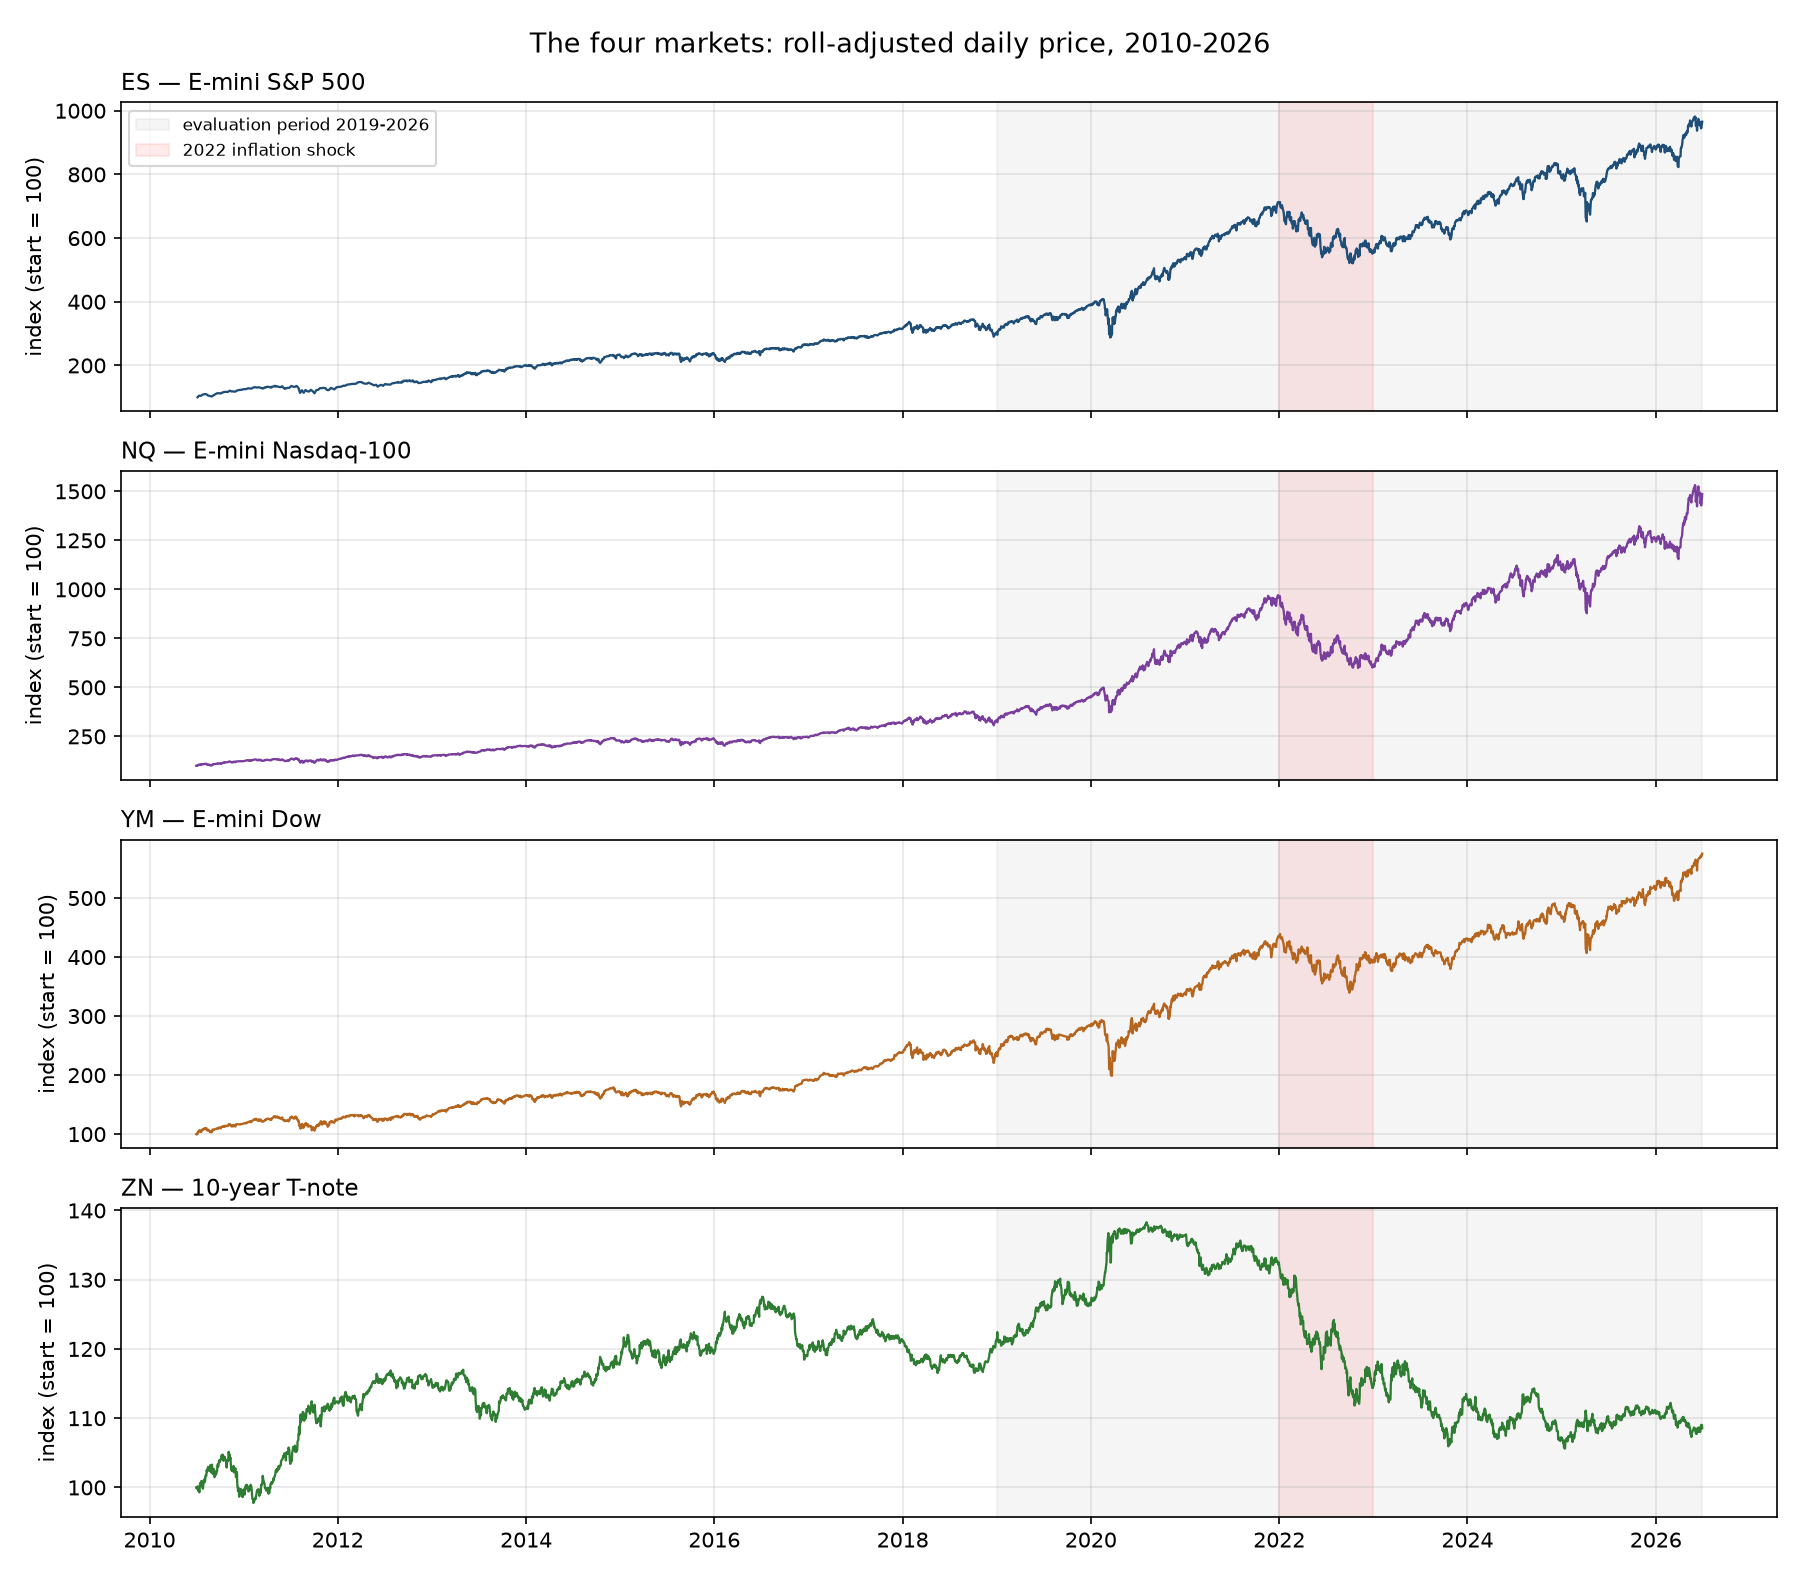
\includegraphics[width=0.85\linewidth]{fig01_markets_overview_4m}
  \caption{\ES, \NQ, \YM\ and \ZN, 2010--2026. Roll-adjusted daily prices rebased to 100. Grey: the
  2019--2026 evaluation period; red: the 2022 inflation shock.}
  \label{fig:markets}
\end{figure}

\subsection{Measuring surprises}

The Bloomberg calendar contains 179 U.S.\ release lines and 27,137 release rows between 2010 and
2026, each with a release time, the actual value and the survey median. For line $l$ at release
$t$, the raw surprise $A_{l,t}-F_{l,t}$ is not comparable across lines (payrolls are measured in
thousands of jobs, CPI in tenths of a percent), so we standardize it causally, using only earlier
releases of the same line:
\begin{equation}\label{eq:z}
  z_{l,t} = \frac{A_{l,t}-F_{l,t}}{\operatorname{sd}\left(A_{l,1}-F_{l,1},\ldots,A_{l,t-1}-F_{l,t-1}\right)},
\end{equation}
requiring at least 24 earlier releases and capping $z$ at $\pm 5$ (0.47\% of the 17,328
standardized surprises are capped). Lines that are released at the same instant---for example the
eight CPI lines---are grouped into a release family $f$ when their release timestamps overlap by at
least 80\%. The family signal is
\begin{equation}\label{eq:x}
  x_{f,t} = \frac{1}{|L_f|}\sum_{l\in L_f} s_l\, z_{l,t},
\end{equation}
where the sign $s_l\in\{-1,+1\}$ is the sign of the slope of a regression of the first-minute
return on $z_{l,t}$, estimated separately for each market on earlier years only. With these signs,
$x_{f,t}>0$ always means good news for the market in question: a strong payrolls print is good
news for \ES\ and bad news for \ZN.

\subsection{Sample}

The event-study sample (Section~\ref{sec:discovery}) contains 363 CPI, NFP and PCE releases from
2016 to 2026. The trading samples use all release families with at least 30 releases (75 families
built from 143 lines). All strategies use the sample split in Table~\ref{tab:split}; the first
three years only build the history that later estimates require.

\begin{table}[htbp]
  \centering\small
  \caption{Sample split.}\label{tab:split}
  \begin{tabular}{lll}
    \toprule
    Period & Years & Use \\
    \midrule
    Burn-in    & 2010--2012 & analogue library and surprise history only \\
    Train      & 2013--2017 & first estimation window \\
    Validation & 2018--2020 & out of sample (walk-forward) \\
    Test       & 2021--2026 & out of sample, reported once \\
    \bottomrule
  \end{tabular}
\end{table}

\section{Price Discovery After Scheduled Releases}\label{sec:discovery}

This section asks how much of the response to a release arrives after the first minute and
whether the surprise predicts it. We define, for a release at minute $T$ and horizon $h$, the
reaction from the last pre-release price and the drift from the first post-release price,
\begin{equation}\label{eq:decomp}
  R_{T,h} = \ln P_{T+h-1} - \ln P_{T-1}, \qquad
  D_{T,h} = \ln P_{T+h-1} - \ln P_{T},
\end{equation}
where $P_\tau$ is the close of the bar labelled $\tau$. The reaction is the sum of the first-minute
jump $R_{T,1}$ and the drift, $R_{T,h}=R_{T,1}+D_{T,h}$. Only the drift can be traded.

\subsection{The jump and the drift}

Figure~\ref{fig:cpi_paths} shows the average cumulative return around CPI releases from 2016 to
2026, separately for hot prints (headline surprise above $+0.5$ standard deviations, 38 releases)
and cool prints (below $-0.5$, 36 releases). Three facts stand out. First, all four markets jump in
the direction theory predicts within the first minute: after hot prints \ES\ falls about 37 bps,
\NQ\ about 55 bps, \YM\ about 31 bps and \ZN\ about 19 bps; after cool prints they rise by about 30,
42, 26 and 23 bps.
Second, the equity indices keep moving in the same direction afterwards. After hot prints \ES\
falls a further 15--18 bps, to about $-55$ bps 30 minutes after the release, and \NQ\ a further 20
bps, to about $-77$ bps; \YM\ falls a further 17 bps, to about $-48$ bps. After cool prints the
continuation is smaller, about 3--6 bps in the three equity indices. Third,
\ZN\ continues by only 4--5 bps after hot prints and slightly reverses after cool prints. Before the
release, all four markets are flat on average: there is no systematic pre-positioning in the 30
minutes before CPI.

\begin{figure}[htbp]
  \centering
  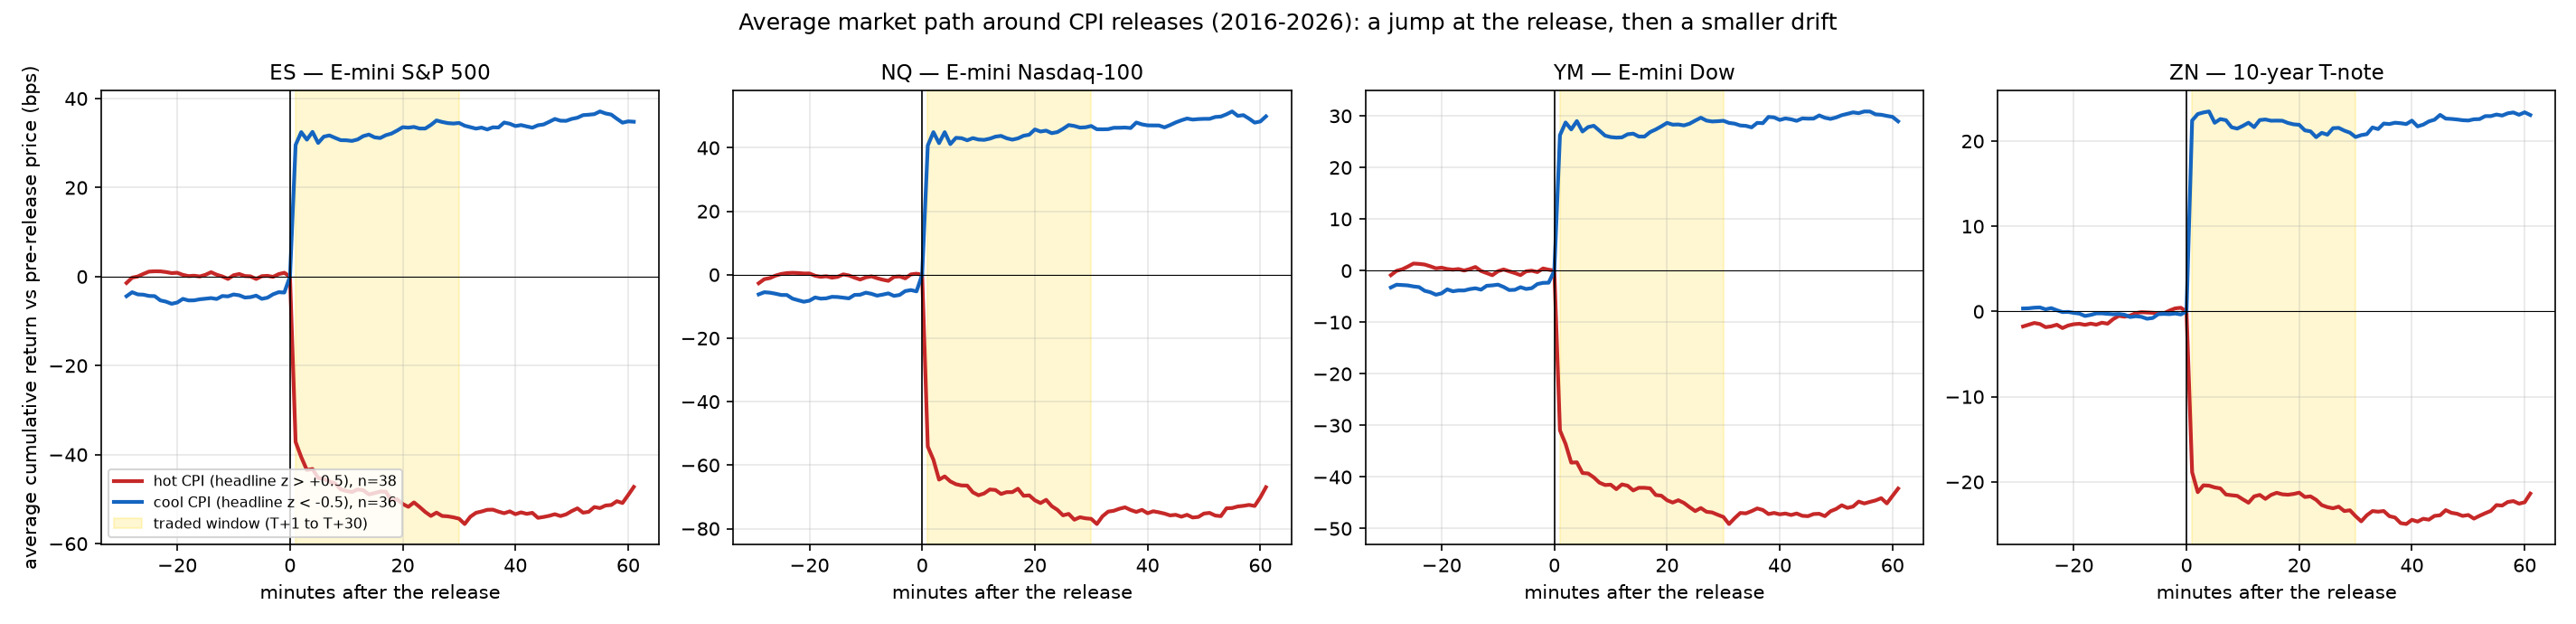
\includegraphics[width=\linewidth]{fig02_cpi_event_paths_4m}
  \caption{Average cumulative return around CPI releases, 2016--2026, relative to the last
  pre-release price, for hot prints (headline surprise above $+0.5$ SD) and cool prints (below
  $-0.5$ SD), \ES, \NQ, \YM\ and \ZN. Shaded: the window a strategy can trade (one to 30 minutes after the release).}
  \label{fig:cpi_paths}
\end{figure}

\subsection{Surprises predict the reaction and the drift}

For each release family we regress the reaction and the drift on the standardized surprise
components with heteroskedasticity-robust (HC3) standard errors. Table~\ref{tab:eventstudy}
reports the results for CPI, NFP and PCE. CPI is the release that matters in all four markets: its
headline surprise explains 27--30\% of the five-minute reaction, with the expected sign. A
one-standard-deviation hot surprise lowers \ES\ by 20.8 bps, \NQ\ by 27.7 bps and \ZN\ by 9.9 bps
over five minutes. \NQ\ reacts about 35\% more than \ES, consistent with the higher rate
sensitivity of long-duration technology stocks, and \YM\ about 8\% less (19.2 bps, $R^2$ 0.27), with
the same drift as \ES\ after the first minute ($-5.3$ against $-5.7$ bps). NFP moves prices almost as much as CPI on average
(30 bps in \ES), but in a direction the surprise hardly explains ($R^2$ of 1--3\%), because
payrolls, the unemployment rate and wages often point in different directions.

\begin{table}[htbp]
  \centering\small
  \caption{Response to CPI, NFP and PCE surprises, 2016--2026.}\label{tab:eventstudy}
  \begin{threeparttable}
  \begin{tabular}{llccccc}
    \toprule
    & & Mean $|R_{T,30}|$ & \multicolumn{2}{c}{5-minute reaction} & \multicolumn{2}{c}{Drift $T{+}1\to T{+}30$} \\
    \cmidrule(lr){4-5}\cmidrule(lr){6-7}
    Market & Release & (bps) & $\beta$ (bps/SD) & $R^2$ & $\beta$ (bps/SD) & $t$ \\
    \midrule
    \ES & CPI & 38.5 & $-20.8$ & 0.27 & $-5.7$  & $-1.4$ \\
    \NQ & CPI & 53.6 & $-27.7$ & 0.30 & $-4.6$  & $-0.9$ \\
    \ZN & CPI & 22.5 & $-9.9$  & 0.30 & $-0.06$ & $-0.04$ \\
    \YM & CPI & 33.2 & $-19.2$ & 0.27 & $-5.3$  & $-1.4$ \\
    \midrule
    \ES & NFP & 29.6 & $+2.8$ & 0.03 & $+0.2$ & 0.1 \\
    \NQ & NFP & 36.0 & $+2.5$ & 0.01 & $-0.6$ & $-0.4$ \\
    \ZN & NFP & 23.6 & $-1.5$ & 0.03 & $+0.1$ & 0.1 \\
    \YM & NFP & 27.9 & $+2.8$ & 0.07 & $+0.6$ & 0.4 \\
    \midrule
    \ES & PCE & 14.9 & $-3.8$ & 0.10 & $+0.4$ & 0.2 \\
    \NQ & PCE & 18.5 & $-5.2$ & 0.10 & $+1.3$ & 0.5 \\
    \ZN & PCE & 8.3  & $-0.9$ & 0.04 & $+0.5$ & 0.5 \\
    \YM & PCE & 11.9 & $-2.9$ & 0.09 & $-0.6$ & $-0.4$ \\
    \bottomrule
  \end{tabular}
  \begin{tablenotes}\footnotesize
    \item Notes: $\beta$ is the coefficient on the headline surprise in a regression of the
    return on all surprise components of the release (CPI: headline and core; NFP: payrolls,
    unemployment rate, average hourly earnings; PCE: headline and core), with HC3 standard errors.
    122 CPI, 122 NFP and 119 PCE releases (348 with complete \YM\ prices).
  \end{tablenotes}
  \end{threeparttable}
\end{table}

The drift regressions are weaker: with about 120 CPI releases, the coefficient on the headline
surprise alone is not individually significant in any market. The drift is better measured with
the family signal in equation~\eqref{eq:x}, which combines all CPI lines. Its correlation with the
five-minute reaction to CPI is 0.51--0.54 in all four markets, and the 30-minute drift per
standard deviation of the signal is about 5.9 bps in \ES, 8.5 bps in \NQ, 4.4 bps in \YM\ and 0.8 bps in
\ZN. Against a five-minute reaction of 27, 37, 22 and 14 bps per standard deviation, between a fifth
and a quarter of the CPI response in the equity indices remains as a drift after the first minute,
and almost none in \ZN.
Figure~\ref{fig:reaction_drift} shows the same contrast. The trading tests in
Section~\ref{sec:results}, which aggregate many releases with walk-forward signs, are the decisive
evidence on whether this drift is predictable out of sample.

\begin{figure}[htbp]
  \centering
  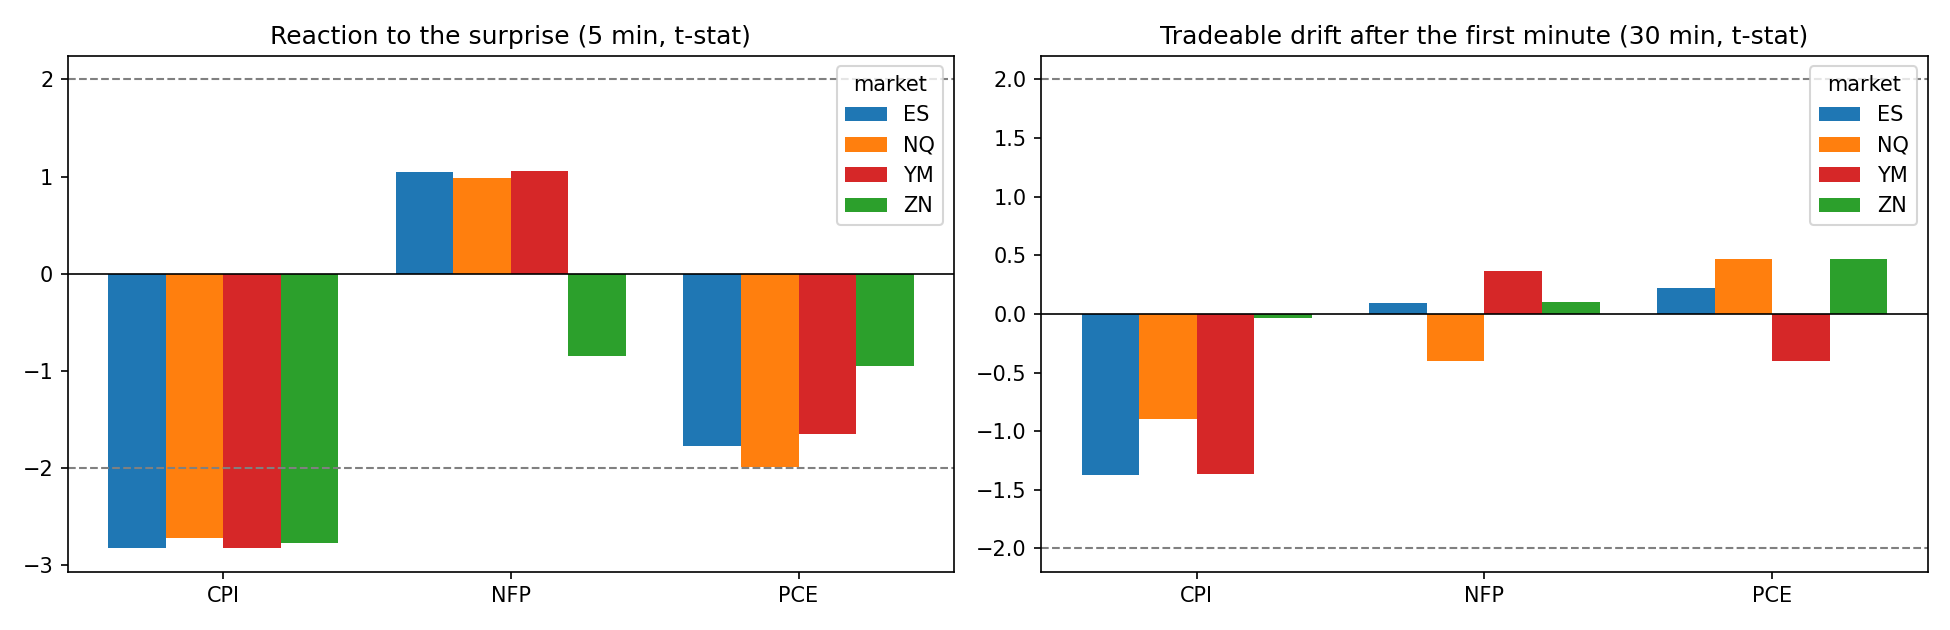
\includegraphics[width=0.9\linewidth]{nb02b_reaction_vs_drift_4markets}
  \caption{$t$-statistics of the headline surprise (CPI, payrolls, PCE) in regressions of the
  five-minute reaction from the pre-release price (left) and of the drift from one to 30 minutes
  after the release (right), \ES, \NQ, \YM\ and \ZN, 2016--2026. Dashed lines: $\pm 2$.}
  \label{fig:reaction_drift}
\end{figure}

\subsection{Does the pre-release market state matter?}

\citet{Andersen2007} show that announcement effects depend on the state of the economy. We ask a
related question at high frequency: does the same surprise move prices more when markets are
already stressed? We pre-register six state variables measured before the release---20-day
realized volatility, the previous day's intraday volatility, 20-day momentum, the distance from the
60-day high, the overnight return and the previous surprise of the same release---each converted
to a percentile against its trailing one-year distribution, and estimate
\begin{equation}\label{eq:state}
  r_T = a + b\,x_T + c\,s_T + d\,(x_T\times s_T) + \varepsilon_T ,
\end{equation}
where $s_T\in[0,1]$ is the state percentile, so $d$ is the change in the surprise beta from the
calmest to the most stressed state. Each interaction is tested with HC3 and a 2,000-draw
permutation test, corrected for the 48 primary tests with the false-discovery rate of
\citet{Benjamini1995}, and required to have the same sign in 2016--2020 and 2021--2026.

\begin{figure}[htbp]
  \centering
  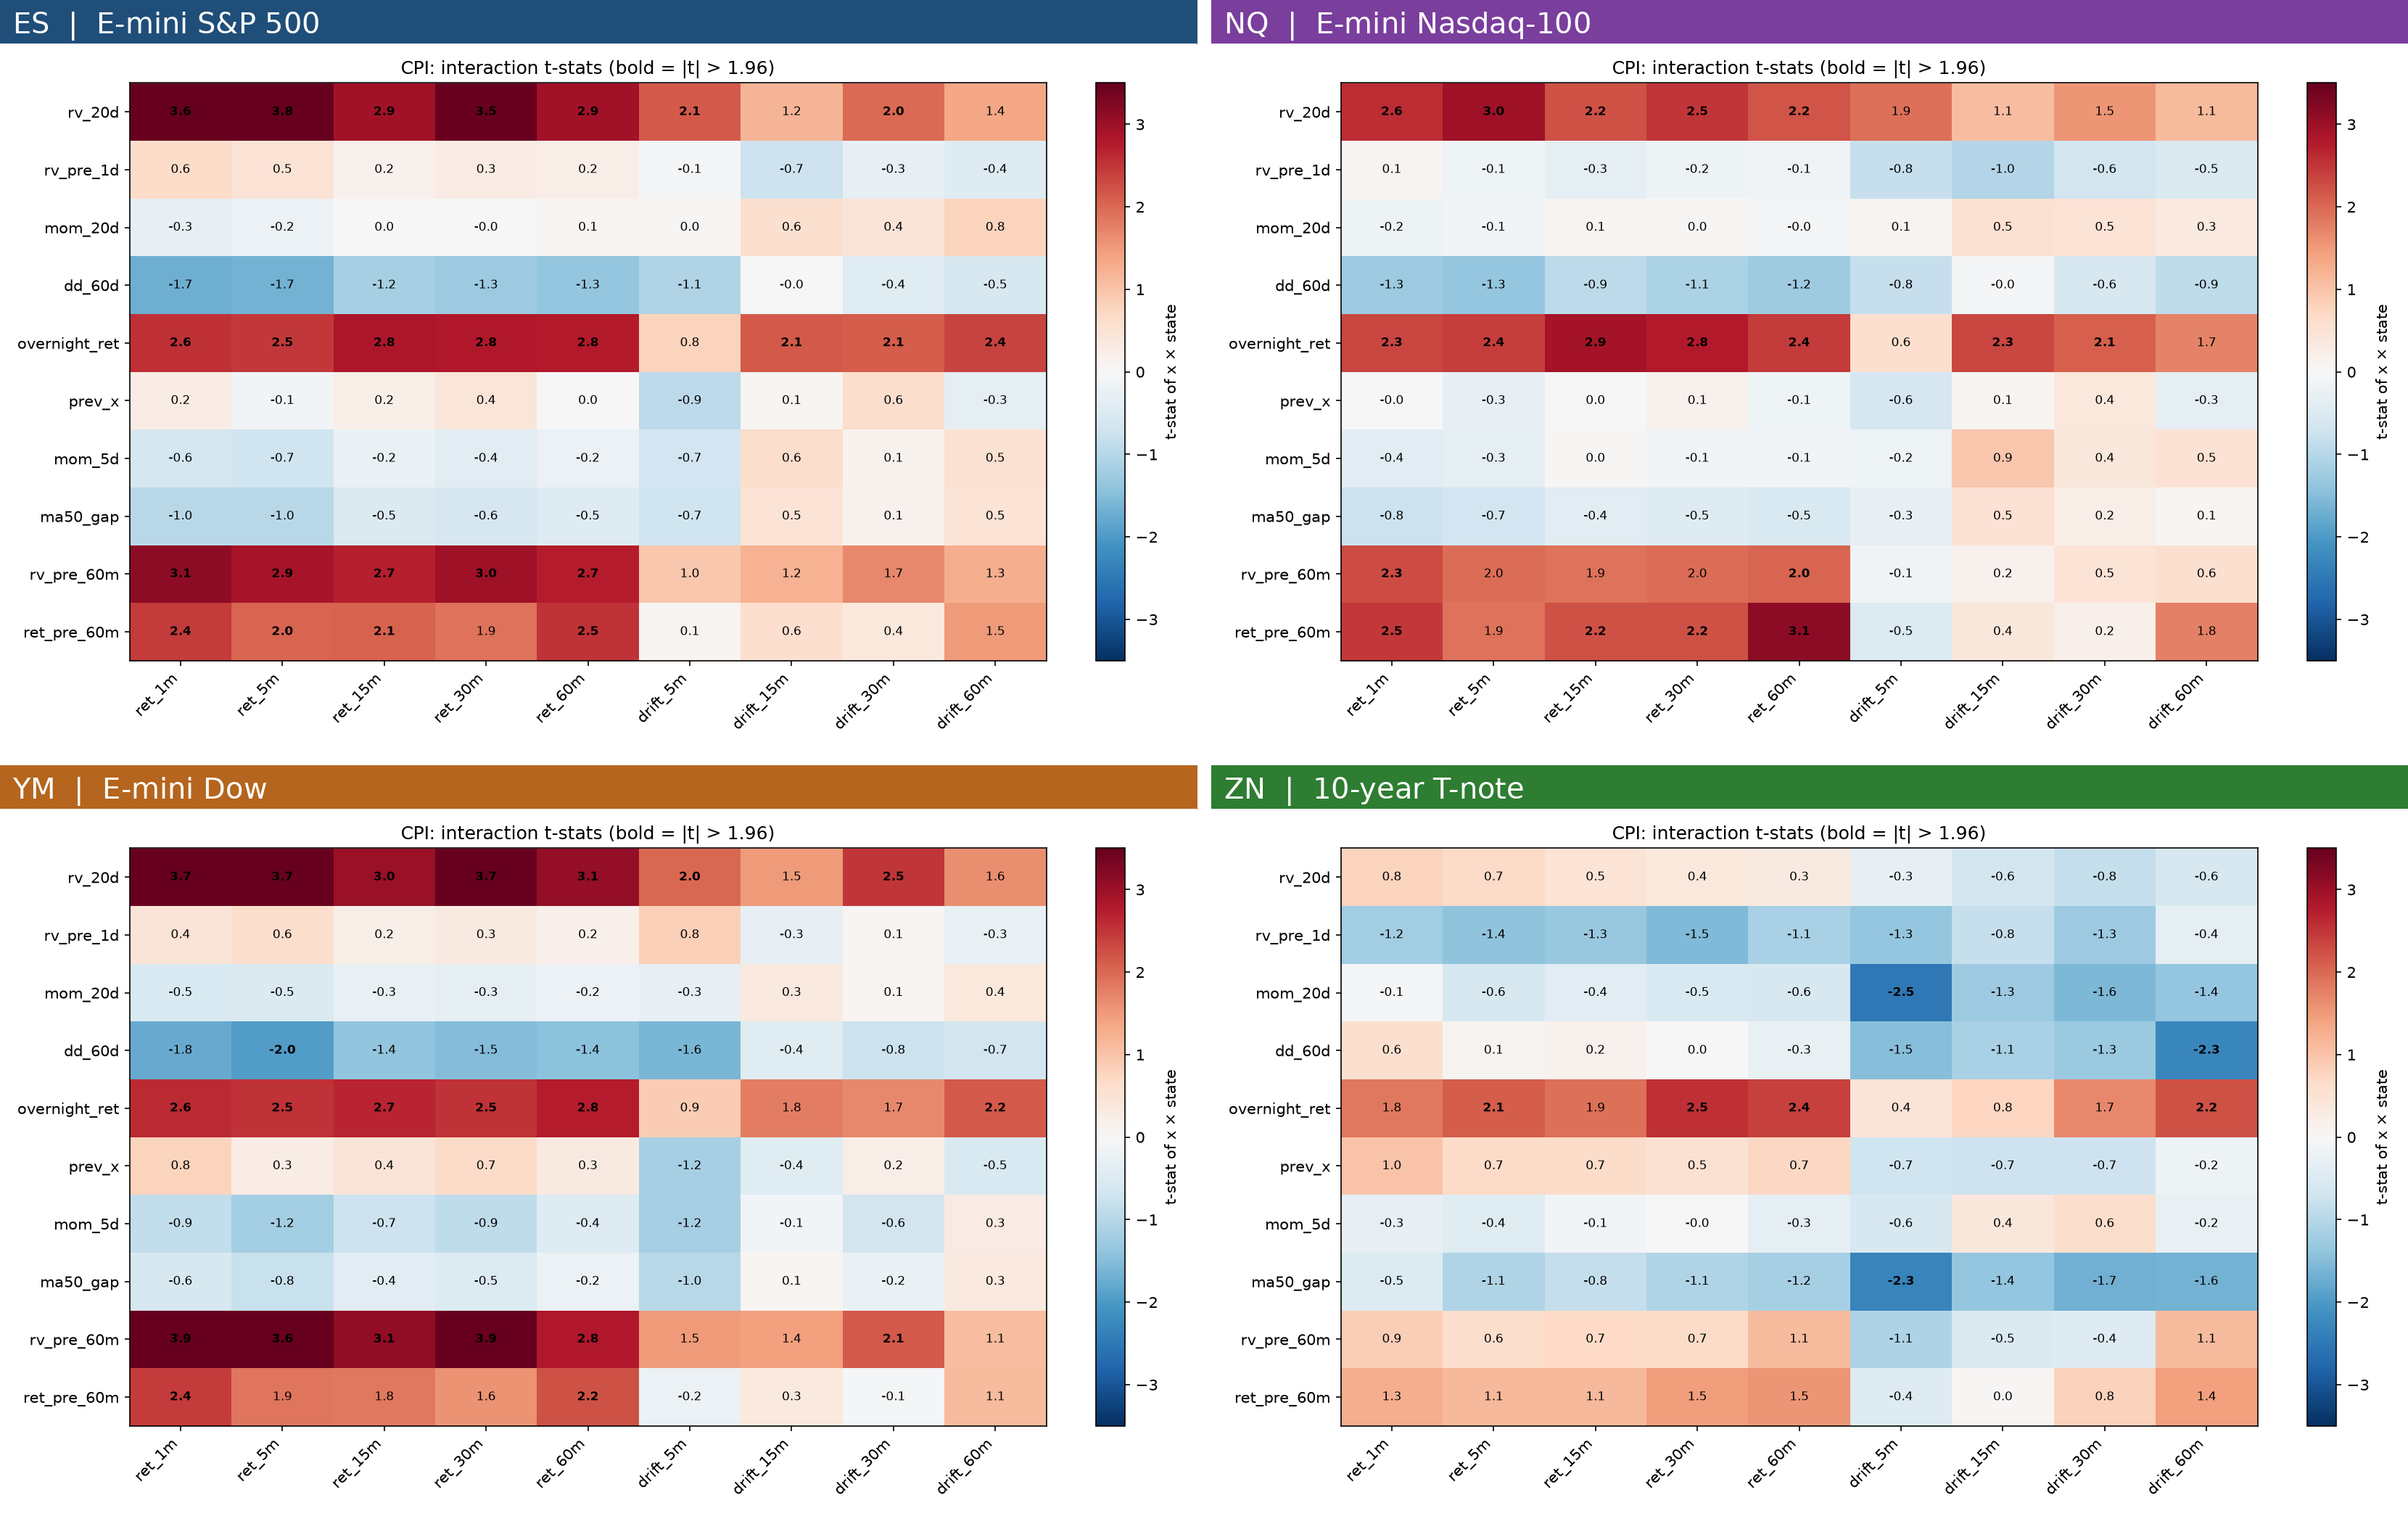
\includegraphics[width=\linewidth]{fig12_interaction_tstats_CPI_4markets}
  \caption{$t$-statistics of the CPI $\times$ state interaction $d$ in equation~\eqref{eq:state},
  by state variable (rows) and target (columns: reactions and drifts at 1--60 minutes), for \ES,
  \NQ, \YM\ and \ZN.}
  \label{fig:state}
\end{figure}

Figure~\ref{fig:state} summarizes the results. In \ES, CPI surprises hit much harder when recent
volatility is high: the interaction with 20-day volatility has $t$-statistics of 2.9--3.8 on the
reactions at every horizon, and the five-minute beta rises by about 61 bps from the calmest to the
most volatile markets. \NQ\ shows the same pattern slightly weaker ($t$ of 2.2--3.0), and \YM\ almost exactly the same
one: its five-minute CPI beta rises by 58.7 bps from calm to volatile states ($t=3.74$,
permutation $p=0.004$), with the same sign in 2016--2020 and 2021--2026. Three features
limit the economic value of this result. First, the effect is concentrated in the first-minute
jump; on the tradeable drift the $t$-statistics fall to 1.1--2.1. Second, in walk-forward estimation
the interaction was not detectable in real time before 2022: its training $t$-statistic was 0.5 in
2019 and below 2 until 2022. Third, only two \ES\ tests and no \NQ\ test survive the false-discovery
correction; in \YM\ three survive, CPI $\times$ volatility and two NFP $\times$ volatility effects
that come entirely from 2016--2020. On the \YM\ drift the CPI interaction is $+24.6$ bps ($t=2.52$)
but does not survive the correction. In \ZN\ there is no volatility pattern at all. The state variables do predict the size
of the move robustly: in high-volatility states the absolute 30-minute move is about 20 bps larger
in \ES, and 198 (\ES), 154 (\NQ) and 156 (\YM) of 360 magnitude tests survive the correction. We return to this
distinction between direction and size in Section~\ref{sec:mechanisms}.

\section{Models and Evaluation}\label{sec:exploit}

This section sets out a simple framework for the speed of price discovery, the common trading
and evaluation environment, and the four forecasting models. Throughout, $T$ denotes the release
minute, $P_\tau$ the close of the one-minute bar labelled $\tau$, $p_\tau=\ln P_\tau$, and
$\mathcal{F}_{T}$ the information available at the close of bar $T$, one minute after the
release. All returns are in basis points (bps).

\subsection{A partial-adjustment framework}\label{sec:framework}

Let $v_T$ denote the change in the fundamental value of the asset implied by the news in a
release, and suppose that it is proportional to the family signal in equation~\eqref{eq:x},
$v_T=\gamma\,x_T$, where $\gamma$ is the full-information price impact of a one-standard-deviation
surprise. Prices adjust toward the new value gradually. We write the cumulative reaction after
$h$ minutes as
\begin{equation}\label{eq:pa}
  R_{T,h} = p_{T+h-1}-p_{T-1} = \Lambda_h\,\gamma\,x_T + u_{T,h},
  \qquad 0\le \Lambda_1 \le \Lambda_2 \le \dots \le 1,
\end{equation}
where $\Lambda_h$ is the share of the news priced after $h$ minutes and $u_{T,h}$ is noise
unrelated to the surprise, $\mathbb{E}[u_{T,h}\mid x_T]=0$. Under efficient and instantaneous
price discovery, $\Lambda_1=1$. Using the decomposition in equation~\eqref{eq:decomp}, the
tradeable drift from the first post-release price is
\begin{equation}\label{eq:drift_model}
  D_{T,h} = R_{T,h}-R_{T,1} = (\Lambda_h-\Lambda_1)\,\gamma\,x_T + (u_{T,h}-u_{T,1}).
\end{equation}
Equation~\eqref{eq:drift_model} delivers the two quantities this paper measures. The first is the
share of the news that is \emph{not} priced within the first minute,
\begin{equation}\label{eq:theta}
  \theta_h \equiv 1-\frac{\Lambda_1}{\Lambda_h}
  = \frac{\beta^{D}_h}{\beta^{R}_h},
  \qquad
  \beta^{R}_h=\frac{\operatorname{Cov}(R_{T,h},x_T)}{\operatorname{Var}(x_T)},\quad
  \beta^{D}_h=\frac{\operatorname{Cov}(D_{T,h},x_T)}{\operatorname{Var}(x_T)},
\end{equation}
which is identified from two predictive regressions. The second is the predictability of the
drift from public information: since $x_T\in\mathcal{F}_T$,
\begin{equation}\label{eq:predict}
  \mathbb{E}\left[D_{T,h}\mid\mathcal{F}_T\right] = \beta^{D}_h\,x_T,
\end{equation}
so a strategy that takes a position in the direction of $x_T$ at the close of bar $T$ earns
$\beta^{D}_h\,\mathbb{E}|x_T|$ per trade before costs. The drift is exploitable only if this
exceeds the round-trip cost $c$,
\begin{equation}\label{eq:exploit}
  \beta^{D}_h\,\mathbb{E}\left|x_T\right| > c .
\end{equation}
Condition~\eqref{eq:exploit} separates two reasons why a predictable drift may not be traded: the
news may be priced almost entirely within a minute ($\theta_h\approx 0$), or the remaining drift
may be small relative to the minimum price increment, which sets a floor on $c$. The average CPI
paths in Section~\ref{sec:discovery} imply $\theta_{30}\approx 0.3$ in \ES, \NQ\ and \YM\ and
$\theta_{30}\approx 0.2$ in \ZN; the estimated drift slopes of about 5.9, 8.5, 4.4 and 0.8 bps per
standard deviation, against round-trip costs of about 1.7, 0.7, 1.0 and 3.0 bps, satisfy
condition~\eqref{eq:exploit} in the three equity markets and violate it in \ZN.

\subsection{Trading environment}\label{sec:environment}

\paragraph{Timing and returns.}
Every model forms its forecast with information in $\mathcal{F}_T$ and opens a position
$w_T\in[-2,2]$ (in contracts) at the close of bar $T$ (Figure~\ref{fig:timing}). A trade on
window $k$ opens at minute $T+a_k$ and closes 30 minutes later, with gross return
\begin{equation}\label{eq:trade}
  r^{g}_{T,k} = w_{T,k}\,\left(p_{T+a_k+29}-p_{T+a_k-1}\right)\times 10^4 ,
\end{equation}
with $a_1=1$ for the single-window models, so that $r^{g}_{T,1}=w_{T,1}D_{T,30}$. The last
pre-release price $p_{T-1}$ is never an entry price.

\begin{figure}[htbp]
  \centering
  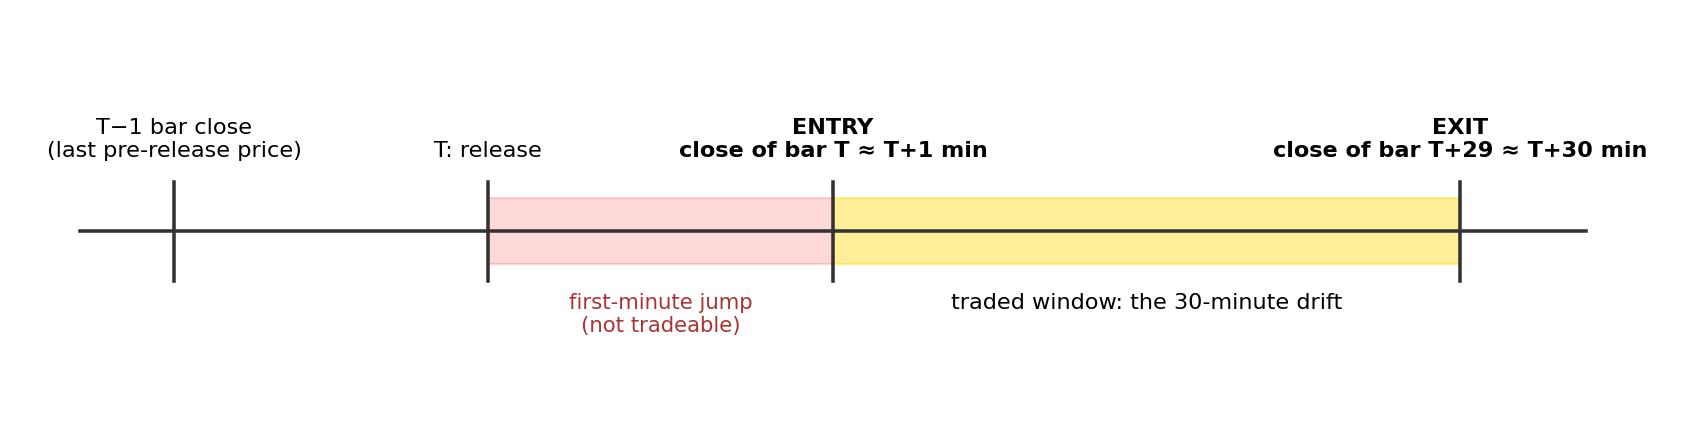
\includegraphics[width=0.85\linewidth]{diagram_timing}
  \caption{Timing of a trade. The release occurs at $T$; the close of bar $T-1$ is the last
  pre-release price; the jump is priced within bar $T$; the position is opened at the close of
  bar $T$ and closed at the close of bar $T+29$.}
  \label{fig:timing}
\end{figure}

\paragraph{Costs.}
For a contract with tick size $\delta$ (in price points) and point value $M$ (in dollars), trading
$n$ ticks of slippage per round trip plus a commission $\kappa$ costs, in basis points of the
entry price $P$,
\begin{equation}\label{eq:cost}
  c(P) = \frac{n\,\delta + \kappa/M}{P}\times 10^4 ,
\end{equation}
and the net return is $r_{T,k}=r^{g}_{T,k}-|w_{T,k}|\,c(P_{T+a_k-1})$. We report $n\in\{0,
\tfrac12, 1\}$ with $\kappa=0$ (gross, a quarter and a half tick per side) and $n=2$, $\kappa=\$4.50$
(the base case).

\paragraph{Performance.}
Let $d(t)$ be the trading session of time $t$ (18:00--17:00 Eastern Time, dated by the close). The
daily P\&L of a book is $\pi_s=\sum_{(T,k):\,d(T+a_k)=s} r_{T,k}$, zero on sessions without a trade.
Over $S$ sessions,
\begin{equation}\label{eq:sharpe}
  \widehat{SR} = \sqrt{252}\,\frac{\bar\pi}{\hat\sigma_\pi},\qquad
  \mathrm{MDD} = \min_{s}\Big(\sum_{j\le s}\pi_j-\max_{u\le s}\sum_{j\le u}\pi_j\Big),\qquad
  \hat\beta = \frac{\widehat{\operatorname{Cov}}(\pi_s,\pi^{BH}_s)}{\widehat{\operatorname{Var}}(\pi^{BH}_s)},
\end{equation}
where $\pi^{BH}_s$ is the daily return of holding one contract, with roll jumps set to zero. The
single-model results in Section~\ref{sec:results}.A report monthly Sharpe ratios, with
$\sqrt{12}$ replacing $\sqrt{252}$.

\paragraph{Out-of-sample estimation.}
Every estimated quantity---line signs, the release universe, regression slopes, gate thresholds
and position-size references---is re-estimated at the start of each year $y$ using only releases
before January 1 of year $y$. We write $\mathcal{H}_y$ for this history. The single-model results
(Section~\ref{sec:results}.A) use history from 2016 and evaluate 2019--2026 at the base cost. The
comparison of the four models (Sections~\ref{sec:results}.C--F) uses the split in
Table~\ref{tab:split} and reports the validation years (2018--2020) and the test years (2021--2026)
separately.

\subsection{Model 1: Consensus surprises}\label{sec:model_surprise}

\paragraph{Line signs.} For each market and line $l$, the sign $s_{l,y}$ in
equation~\eqref{eq:x} is the sign of the OLS slope of the first-minute jump on the standardized
surprise over $\mathcal{H}_y$,
\begin{equation}\label{eq:sign}
  R_{T,1} = a_l + b_l\, z_{l,T} + e_{T},\qquad s_{l,y}=\operatorname{sign}\big(\hat b_{l}\big),
\end{equation}
estimated when at least 24 releases are available.

\paragraph{Release universe.} For each family $f$ and year $y$, an impact screen compares the
family's 30-minute reaction to that of other families released at the same clock time,
\begin{equation}\label{eq:impact}
  I_{f,y} = \frac{\operatorname{mean}_{T\in\mathcal{T}_{f}\cap\mathcal{H}_y}\,|R_{T,30}|}
  {\operatorname{mean}_{T\in\mathcal{C}_{f}\cap\mathcal{H}_y}\,|R_{T,30}|},
\end{equation}
where $\mathcal{T}_f$ are the family's release times and $\mathcal{C}_f$ the release times of other
families at the family's modal clock time on which $f$ is not released. The ten families with the
largest $I_{f,y}$ (at least 30 releases each), plus CPI, form the universe $\mathcal{U}_y$.

\paragraph{Naive book.} For every $f\in\mathcal{U}_y$ released at $T$,
\begin{equation}\label{eq:naive}
  w_{f,T} = \operatorname{sign}\left(x_{f,T}\right),\qquad
  w_T = \frac{1}{|\mathcal{U}_T|}\sum_{f\in\mathcal{U}_T} w_{f,T},
\end{equation}
where $\mathcal{U}_T$ is the set of universe families released at the same minute, so no minute is
traded twice.

\paragraph{CPI model.} For CPI, the drift slope in equation~\eqref{eq:predict} is estimated on
the earlier CPI releases $\mathcal{H}_T=\{t<T\}$,
\begin{equation}\label{eq:cpimodel}
  \hat\beta^{D}_{T} = \arg\min_{b}\sum_{t\in\mathcal{H}_T}\big(D_{t,30}-b\,x_{t}\big)^2,
  \qquad \hat r_T=\hat\beta^{D}_{T}\,x_T,
\end{equation}
requiring at least 24 earlier releases, and the position implements
condition~\eqref{eq:exploit} release by release:
\begin{equation}\label{eq:cpitrade}
  w_T = \operatorname{sign}(\hat r_T)\,\mathbf{1}\big\{|\hat r_T| > c(P_{T})\big\}.
\end{equation}

\subsection{Model 2: Price-path analogues (DTW ladder)}\label{sec:model_dtw}

\paragraph{Paths.} For a trade entering at minute $e=T+a_k$, the query path is the log price over
the $L+1=31$ minutes ending at the entry, standardized so that only its shape matters,
\begin{equation}\label{eq:path}
  q_j = \frac{p_{e-L+j-1}-\bar p}{\hat\sigma_p},\qquad j=1,\dots,L+1 ,
\end{equation}
where $\bar p$ and $\hat\sigma_p$ are the mean and standard deviation of the $L+1$ log prices.

\paragraph{Distance.} For two standardized paths $q$ and $c$ of length $n$, the dynamic time
warping distance is computed by the recursion
\begin{equation}\label{eq:dtw}
  g(i,j) = (q_i-c_j)^2 + \min\{g(i-1,j),\,g(i,j-1),\,g(i-1,j-1)\},
  \qquad |i-j|\le b,
\end{equation}
with $g(0,0)=0$, $g(i,0)=g(0,j)=\infty$ and $d(q,c)=g(n,n)$. The Sakoe--Chiba band $b=5$ minutes
allows the reaction to unfold up to five minutes faster or slower than in the matched past
episode \citep{Sakoe1978, Berndt1994}.

\paragraph{Neighbours and forecasts.} The candidate set $\mathcal{N}_e$ contains the paths of
earlier releases at the same clock time and window $k$, within a three-year lookback, whose own
trade closed before $e$, limited to the 600 most recent. With $\mathcal{K}_e\subset\mathcal{N}_e$
the $K=15$ candidates with the smallest distances $d_j$, ages $\tau_j$ in years and realized
next-30-minute returns $y_j$, the weights and the two forecasts are
\begin{equation}\label{eq:dtwforecast}
  \omega_j = \frac{d_j^{-1}\,2^{-\tau_j/H}}{\sum_{i\in\mathcal{K}_e} d_i^{-1}\,2^{-\tau_i/H}},\qquad
  \mu_e = \sum_{j\in\mathcal{K}_e}\omega_j\,y_j,\qquad
  \sigma_e = \Big(\sum_{j\in\mathcal{K}_e}\omega_j\,(y_j-\mu_e)^2\Big)^{1/2},
\end{equation}
with a recency half-life of $H=2$ years. The direction forecast $\mu_e$ is the analogue estimate of
$\mathbb{E}[D\mid\text{path}]$ and the dispersion forecast $\sigma_e$ measures how much the analogues
disagree.

\paragraph{Gate and size.} With $Q_\alpha$ the $\alpha$-quantile of $\mu$ over the fitting years and
$\bar\sigma$ the median of $\sigma$,
\begin{equation}\label{eq:dtwtrade}
  w_e = \operatorname{sign}(\mu_e)\,\mathbf{1}\big\{\mu_e\le Q_{0.3}\ \text{or}\ \mu_e\ge Q_{0.7}\big\}
  \cdot \min\Big\{\frac{\bar\sigma}{\sigma_e},\,2\Big\}.
\end{equation}
The book trades five back-to-back windows after each release of eight families, $a_k\in\{1,31,61,
91,121\}$, with the forecasts in equation~\eqref{eq:dtwforecast} rebuilt for each window.

\subsection{Model 3: Pattern-based event games}\label{sec:model_games}

The event-game model applies the analogue logic to longer paths around the release. For each
release $T$ and anchor $T_0=T+o$, $o\in\{-60,-30,0,30,60\}$ minutes, the path is the log return
over $[T_0,T_0+60]$ sampled every $\Delta=3$ minutes and standardized as in
equation~\eqref{eq:path}, and the target is the next 30-minute return,
\begin{equation}\label{eq:game}
  y_{T,o} = p_{T_0+90}-p_{T_0+60}.
\end{equation}
Neighbours come from a pool $\mathcal{P}$ of release types (Jobless Claims, JOLTS and PCE) at the
same clock time and anchor, within a two-year lookback, with a DTW band of five sampling steps. The
factor is the distance- and recency-weighted average of the neighbours' targets, as in
equation~\eqref{eq:dtwforecast}, and the book trades
\begin{equation}\label{eq:gametrade}
  w_{T,o}=\operatorname{sign}\big(\mu_{T,o}\big)
\end{equation}
one contract, entering at $T_0+60$. The pool, sampling frequency and lookback were chosen by a grid
search over 18 combinations on the full sample.

\subsection{Model 4: Machine-learning classifier}\label{sec:model_ml}

The classifier forecasts the direction of the 30-minute return from a feature vector $\phi_T$
that combines surprise, price-path and momentum information. With $\hat F_y$ trained on
$\mathcal{H}_y$,
\begin{equation}\label{eq:ml}
  \hat\rho_T = \Pr\nolimits_{\hat F_y}\left(D_{T,30}>0 \mid \phi_T\right),\qquad
  w_T = g\big(\hat\rho_T\big)\in[-1,1],
\end{equation}
where $g$ maps the predicted probability into a signed position that is larger when the model is
more confident; we keep the model's positions exactly as produced. The \emph{executable} version
uses the trade return in equation~\eqref{eq:trade} with $a_1=1$. The \emph{as-reported} version
enters at the last pre-release price,
\begin{equation}\label{eq:asreported}
  r^{g,\text{rep}}_{T} = w_T\,\big(p_{T+28}-p_{T-1}\big)\times 10^4 = w_T\,\big(R_{T,1}+D_{T,29}\big)\times 10^4 ,
\end{equation}
so the difference between the two isolates the value of the untradeable first-minute jump
$R_{T,1}$, which by equation~\eqref{eq:pa} contains the share $\Lambda_1$ of the news.

\subsection{Inference}\label{sec:inference}

\paragraph{Random-sign test.} Holding the trades, sizes and costs of a book fixed, we draw
$\epsilon_{T,k}\in\{-1,+1\}$ with equal probability and form
$\tilde r_{T,k}=\epsilon_{T,k}\,|w_{T,k}|\,(p_{T+a_k+29}-p_{T+a_k-1})\times10^4-|w_{T,k}|\,c$. With
$\widehat{SR}^{(b)}$ the Sharpe ratio of the $b$-th of $B=1{,}000$ draws,
\begin{equation}\label{eq:randsign}
  p_{\text{RS}} = \frac{1}{B}\sum_{b=1}^{B}\mathbf{1}\big\{\widehat{SR}^{(b)}\ge\widehat{SR}\big\},
\end{equation}
which tests whether the direction adds value beyond being in the market at release times.

\paragraph{Block bootstrap.} Confidence intervals for $\widehat{SR}$ resample blocks of three
consecutive months of returns with replacement \citep{Kunsch1989}, which preserves serial
dependence in the monthly returns.

\paragraph{Leak test.} For the analogue models we deliberately extend the query path in
equation~\eqref{eq:path} five minutes past the entry. Because the extended path overlaps the
target, performance must rise sharply if the timing is correct; an unchanged result would indicate
that the real book already uses future prices.

\subsection{Combining the models}\label{sec:model_portfolio}

Let $\pi_{i,s}$ be the daily net P\&L of book $i$ at a quarter tick per side and $\hat\sigma_i$ its
standard deviation over the validation years 2018--2020. An equal-risk portfolio of a set of books
$\mathcal{B}$ has daily return
\begin{equation}\label{eq:portfolio}
  \pi^{P}_s = \sum_{i\in\mathcal{B}} \lambda_i\,\pi_{i,s},\qquad
  \lambda_i=\frac{\hat\sigma_i^{-1}}{\sum_{j\in\mathcal{B}}\hat\sigma_j^{-1}},
\end{equation}
and is scored on the test years only. For uncorrelated books with equal Sharpe ratios $SR$, the
portfolio Sharpe ratio is $\sqrt{|\mathcal{B}|}\,SR$; the gain from combining the four models
therefore depends on how correlated their daily returns are and on how much each loses after costs.

\section{Results}\label{sec:results}

\subsection{Consensus surprises forecast the drift}

We first evaluate the surprise approach on its own, walk-forward over 2019--2026 at our base cost
of two ticks plus \$4.50. Trading the sign of the CPI headline surprise earns a net Sharpe ratio
of 1.03 in \ES\ and 1.00 in \NQ, with 9.8 and 13.6 bps per trade over about 86 and 79 releases. The
CPI model, which trades only when the predicted move exceeds the cost, earns 0.99 in \ES\ and 0.79
in \NQ, with hit rates of 64\% and 58\%. The same rule on the E-mini Dow, a market added after the
\ES\ and \NQ\ results were known, earns 0.99 (77 trades, hit rate 57\%). The 90\% block-bootstrap confidence interval of the \ES\
Sharpe ratio is 0.25 to 1.72. In the format common among practitioners, the \ES\ CPI strategy gains
6.6\% of notional while being long in exactly the same 30-minute windows loses 6.0\%; in \NQ\ the
figures are $+7.5\%$ and $-5.4\%$. The profit therefore comes from the direction of the surprise,
not from being in the market at release times. In \ZN\ the naive rule earns 2.7 bps per trade
before costs (gross Sharpe 0.53) and $-0.3$ bps after them; the CPI model correctly declines to
trade.

Trading the ten screened families rather than CPI alone raises the number of trades tenfold, to 98
a year in \ES\ and 97 in \NQ, with net Sharpe ratios of 0.65 and 0.71, 1.7 and 2.4 bps per trade, and
random-sign $p$-values below 0.001 and of 0.005. CPI remains the largest contributor in both markets
($+4.3\%$ and $+6.0\%$ of notional); behind it the ranking of families differs between \ES\ and \NQ,
so the broad book should be read as diversification across many small edges. On \YM\ the broad book
earns 0.68 (about 93 trades a year, random-sign $p=0.006$). Combining \ES\ and \NQ\ gives about 195
trades a year and a Sharpe ratio of 0.72 (random-sign $p<0.001$); adding \YM\ gives about 290 trades
and 0.78, with a 90\% confidence interval of 0.10 to 1.50.

\subsection{Transaction costs and turnover}

Figure~\ref{fig:costs} shows how the CPI strategy's Sharpe ratio changes as the round-trip
slippage rises from zero to eight ticks. The line falls gently in \ES\ (1.15 to 0.62) and is almost
flat in \NQ\ (1.02 to 0.81), because one \NQ\ tick is only 0.1--0.3 bps of the contract value. \YM,
whose tick is about 0.25--1 bp, sits between them (1.06 to 0.81). In \ZN\ the naive rule crosses
zero at about two ticks. For the broad book, the \ES\ Sharpe ratio falls from 1.09 gross to 0.20 at
four ticks, while \NQ\ stays at 0.60 and \YM\ falls from 0.91 to 0.45. Cost robustness is therefore a
property of the market's tick size relative to its post-release moves, not only of the strategy.

\begin{figure}[htbp]
  \centering
  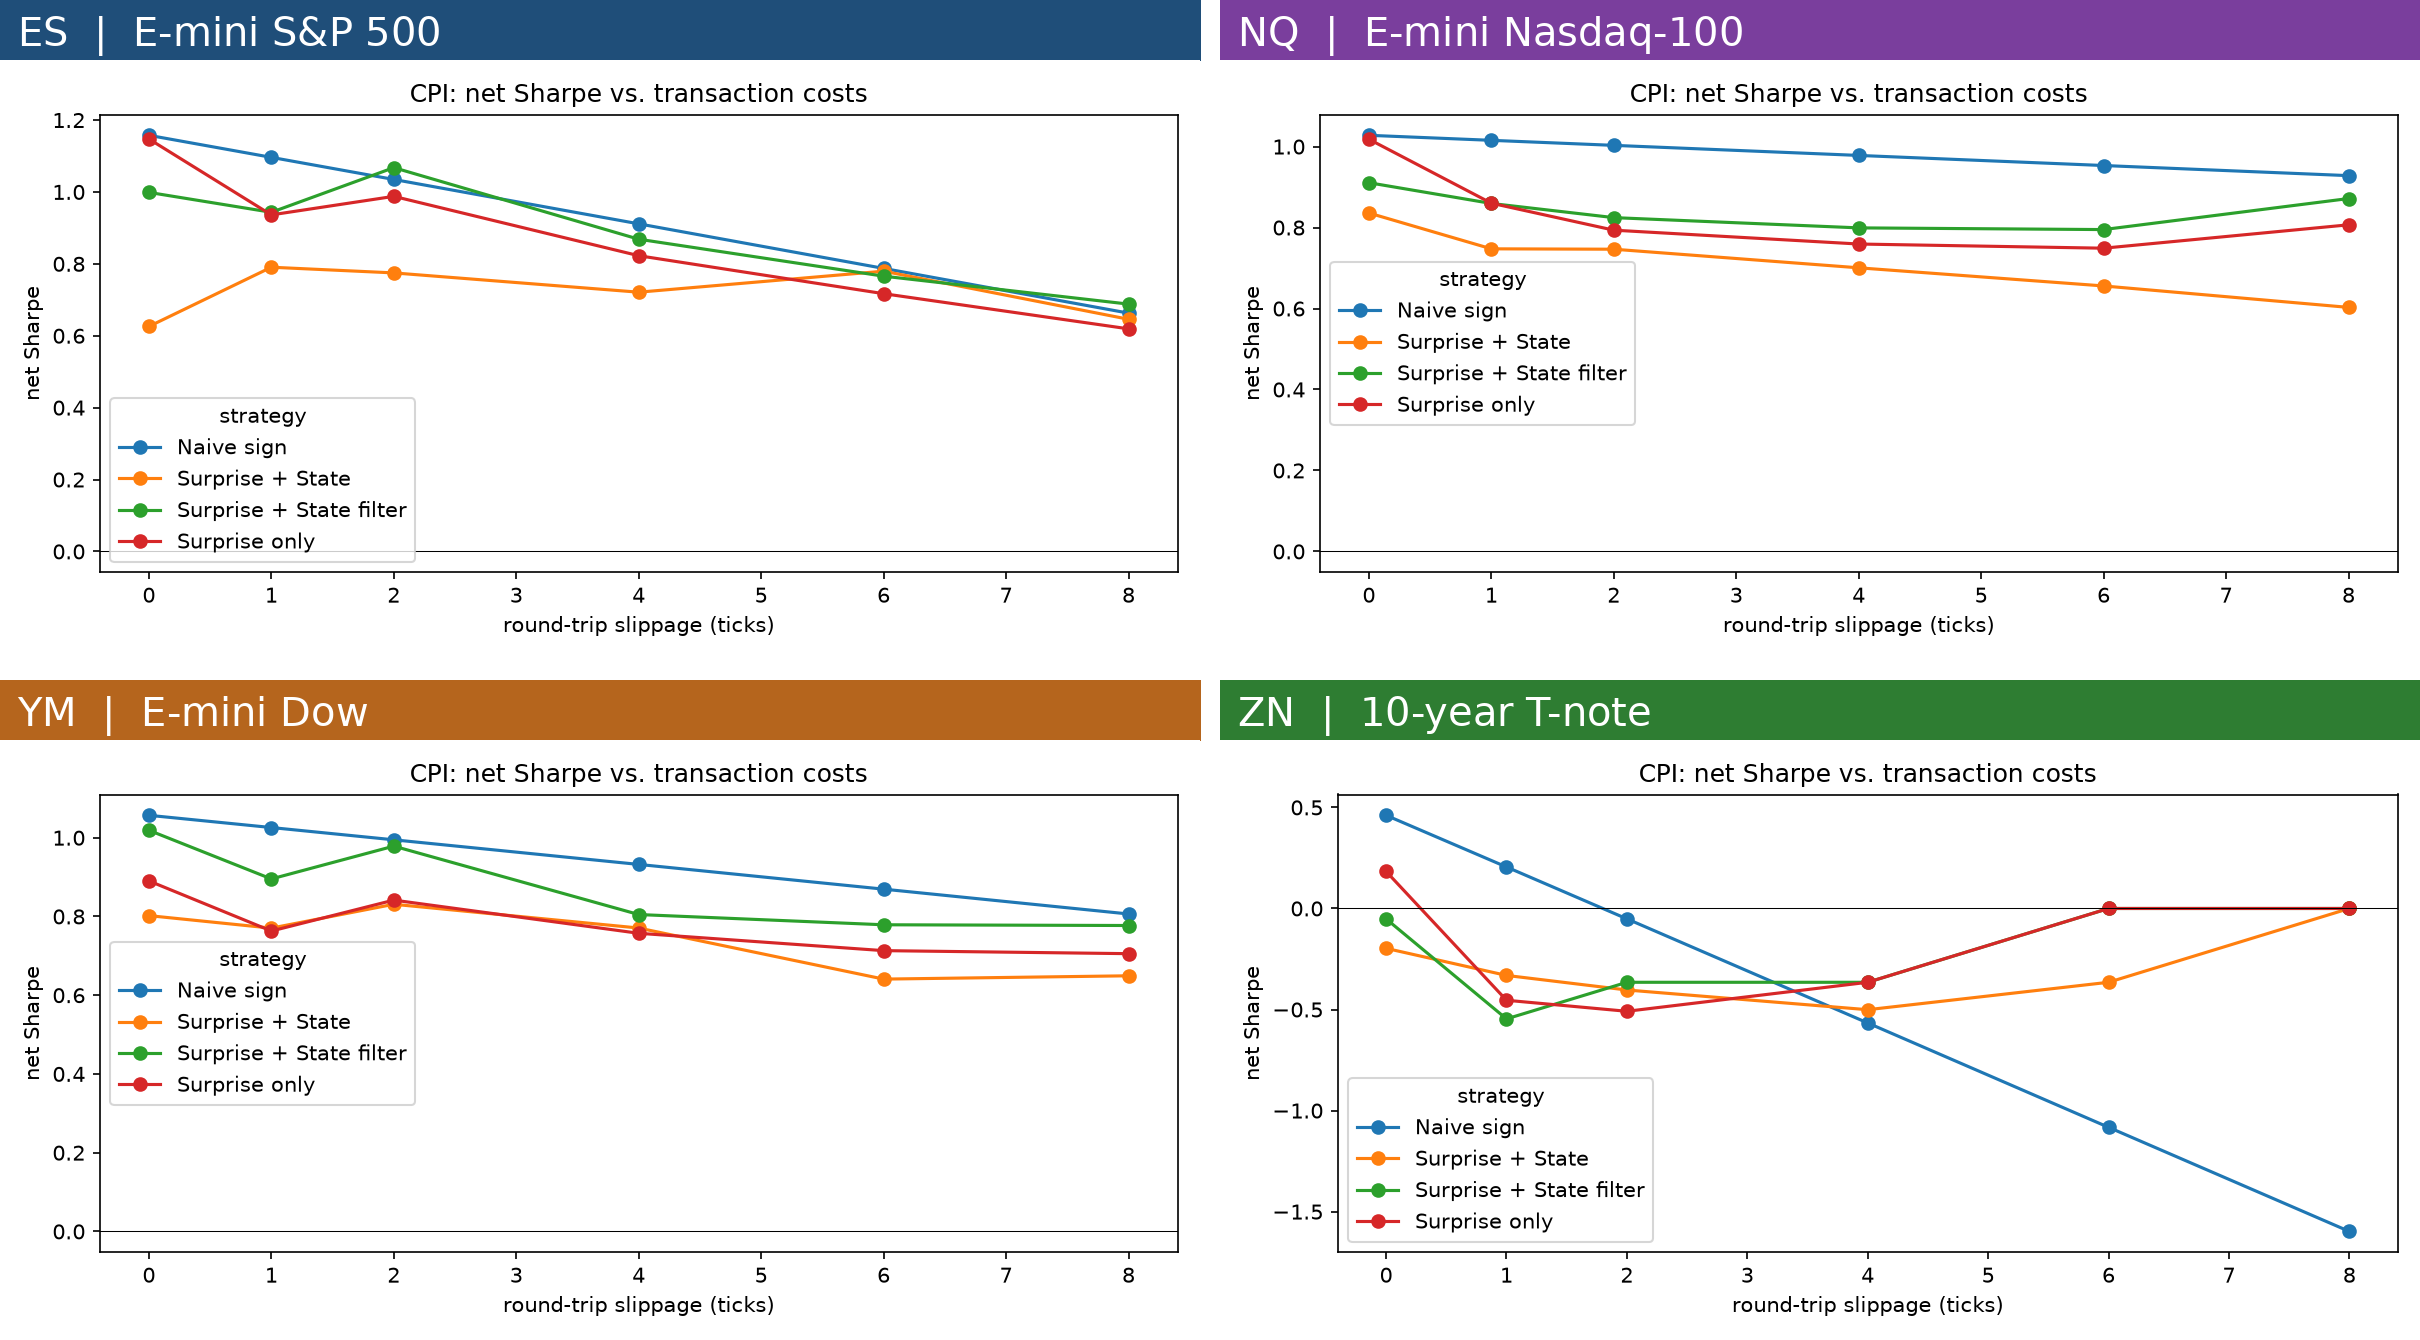
\includegraphics[width=\linewidth]{fig20_cost_sensitivity_4markets}
  \caption{Net Sharpe ratio of the CPI strategies as round-trip slippage rises from 0 to 8 ticks
  (plus a \$4.50 commission), \ES, \NQ, \YM\ and \ZN, 2019--2026.}
  \label{fig:costs}
\end{figure}

\subsection{Four approaches on equal terms}

Table~\ref{tab:strategies} compares the four approaches on the held-out years 2021--2026 with
the same bars, entry, costs and metrics. At a quarter tick per side, the surprise book has the
highest Sharpe ratio in \ES\ (1.09), \NQ\ (0.75) and \YM\ (1.06), followed in \ES\ by the classifier
(0.95), the DTW ladder (0.64) and the event games (0.42). At our base cost the ranking changes: the
classifier (0.81) and the surprise book (0.74) remain clearly positive, the DTW ladder falls to
0.10, and the event games, which trade about 370 times a year, turn negative. In \ZN\ every
approach loses money after costs, although the DTW ladder earns a gross Sharpe ratio of 0.34. On
\YM\ the DTW ladder, run with the same code and setting, loses even before costs ($-0.32$ gross,
$-0.39$ at a quarter tick), while the surprise book earns 1.06: the third equity index confirms the
surprise and not the price-path analogues. The
surprise book is positive in both the validation and the test years on every equity market (\ES\
1.04 and 1.09, \NQ\ 0.86 and 0.75, \YM\ 1.27 and 1.06).

\begin{table}[htbp]
  \centering\small
  \caption{Sharpe ratio of each strategy on each market, test years 2021--2026. ``--'' = the
  strategy is not available on that market.}
  \label{tab:strategies}
  \begin{threeparttable}
  \setlength{\tabcolsep}{4pt}
  \begin{tabular}{lccccccccc}
    \toprule
    & \multicolumn{4}{c}{$\tfrac14$ tick per side} & \multicolumn{4}{c}{2 ticks + \$4.50} & Valid. \\
    \cmidrule(lr){2-5}\cmidrule(lr){6-9}\cmidrule(lr){10-10}
    Strategy & \ES & \NQ & \ZN & \YM & \ES & \NQ & \ZN & \YM & \ES \\
    \midrule
    Macro-surprise book         & 1.09 & 0.75 & $-0.16$ & 1.06 & 0.74 & 0.64 & $-1.51$ & 0.82 & 1.04 \\
    CPI surprise model          & 0.51 & 0.46 & 0.17    & 0.39 & 0.61 & 0.45 & $-0.43$ & 0.29 & 1.27 \\
    DTW ladder book             & 0.64 & 0.11 & $-0.97$ & $-0.39$ & 0.10 & $-0.04$ & $-5.03$ & $-0.74$ & 0.59 \\
    DTW event-game book         & 0.42 & -- & -- & -- & $-0.29$ & -- & -- & -- & 0.26 \\
    Machine-learning classifier & 0.95 & -- & -- & -- & 0.81 & -- & -- & -- & 0.38 \\
    \midrule
    Buy and hold (no costs)     & 0.69 & 0.58 & $-0.69$ & 0.67 & & & & & 0.80 \\
    \bottomrule
  \end{tabular}
  \begin{tablenotes}\footnotesize
    \item Notes: Daily Sharpe ratios on the session grid. The DTW ladder uses the authors' own feature
    panel and rule; the validation column reports 2018--2020 at $\tfrac14$ tick per side.
  \end{tablenotes}
  \end{threeparttable}
\end{table}


\subsection{Combining surprises and price-path analogues}

If the price path before the entry carried information beyond the surprise, conditioning the
surprise on the analogues should improve it. It does not. Across all releases from 2019 to 2026, the
rank correlation of the DTW direction forecast with the next 30-minute return is 0.010 in \ES,
0.026 in \NQ, 0.030 in \YM\ and 0.039 in \ZN, its hit rate is 47--51\%, and its correlation with the
surprise is 0.02--0.13. In the held-out comparison (Figure~\ref{fig:surprise_dtw}), keeping a surprise trade only
when the analogues agree raises the \ES\ Sharpe ratio in the validation years (1.46 against 1.04)
but lowers it in the test years (0.37 against 1.09); \NQ\ shows the same reversal (1.21 against 0.86,
then 0.48 against 0.75). The reason is that the direction of the analogues itself changed sign: the
DTW-only book earned 0.57 (\ES) and 0.78 (\NQ) in 2018--2020 and $-0.26$ and $-0.28$ in 2021--2026.
\YM\ does not show the reversal, but it does not show a gain either: its DTW-only book earns 0.40
and 0.44 in the two periods, and the agreement filter lowers the surprise book in the validation
years (0.63 against 1.27) and leaves it unchanged in the test years (1.04 against 1.06). In the
walk-forward evaluation on 2019--2026 a blend of the two signals raised the \YM\ broad book from
0.68 to 1.06, but the bootstrap probability that it is not better is 6\%, and the same blend does
not help in \ES\ or \NQ. A filter that helps in only one of two periods, or on one of three equity
indices, is not a reliable source of information. In
contrast, the dispersion of the analogues predicts the size of the next move with a rank
correlation of 0.10--0.30 in every market and year, and sizing surprise trades inversely to it
gives Sharpe ratios of 0.63 and 0.72 in \ES\ and 0.64 and 0.97 in \NQ\ in the training and validation
years.

\begin{figure}[htbp]
  \centering
  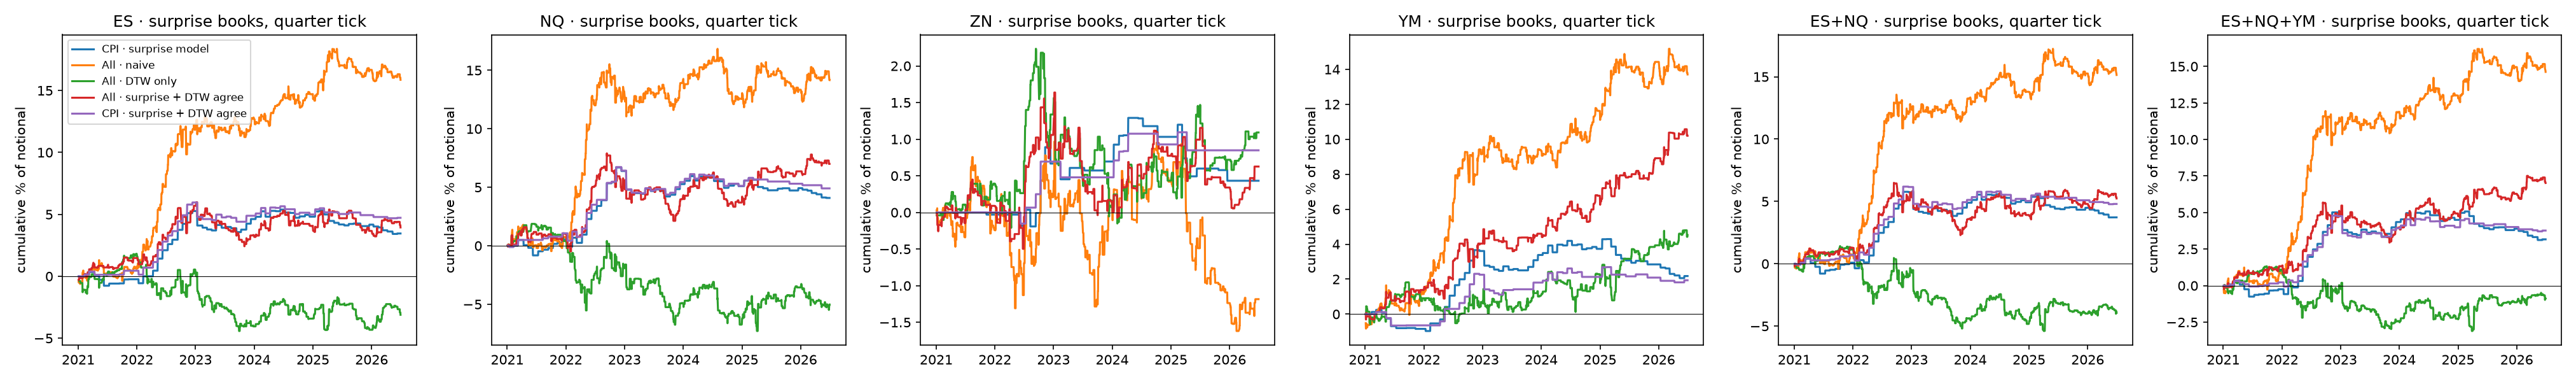
\includegraphics[width=\linewidth]{surprise_dtw_book_cumulative}
  \caption{Cumulative net P\&L at a quarter tick per side, 2021--2026, of the surprise books
  (top-10 families and CPI model), the DTW-only book and the surprise books filtered by DTW
  agreement, in \ES, \NQ, \ZN, \YM\ and equal-risk \ES\ + \NQ\ and \ES\ + \NQ\ + \YM\ books.}
  \label{fig:surprise_dtw}
\end{figure}

\subsection{The entry assumption}

Table~\ref{tab:equalcosts} re-prices each approach's own \ES\ book on 2019--2026 at three cost
levels. The classifier's reported Sharpe ratio of 2.14 (total return 38.6\% gross) falls to 0.92
(7.3\%) when the same positions are entered one minute later: about 80\% of the reported profit is
the first-minute jump. An independent rebuild of the classifier's pipeline finds a loss of about
96\% of the profit per trade from the same one-minute delay. The first minute is where the market
prices the news, and it cannot be traded.

\begin{table}[htbp]
  \centering\small
  \caption{Each workstream's own book re-priced at three cost levels, \ES, 2019--2026
  (Sharpe / total return).}
  \label{tab:equalcosts}
  \begin{tabular}{lccc}
    \toprule
    Book & Gross & $\tfrac14$ tick & 2 ticks + \$4.50 \\
    \midrule
    Macro-surprise, all releases & 1.23 / 23.3\% & 1.12 / 21.1\% & 0.69 / 13.0\% \\
    DTW ladder (2018 \ES\ rebuild)$^{a}$ & 0.27 / 8.8\%  & 0.07 / 2.4\%  & $-0.66$ / $-21.5\%$ \\
    DTW event games              & 0.45 / 18.6\% & 0.25 / 10.3\% & $-0.50$ / $-20.6\%$ \\
    Classifier, executable       & 0.92 / 7.3\%  & 0.88 / 6.9\%  & 0.72 / 5.6\% \\
    Classifier, as reported      & 2.14 / 38.6\% & 2.13 / 38.3\% & 2.07 / 37.0\% \\
    \bottomrule
  \end{tabular}
  \par\smallskip\footnotesize $^{a}$ Rebuilt from the published 2018 specification; the current
  book is in Table~\ref{tab:strategies}.
\end{table}


\subsection{Diversification across approaches}

Daily returns of the four approaches are nearly uncorrelated. In the test years the correlations
across approaches range from $-0.04$ to 0.31, the highest being between the surprise book and the
classifier, which also uses surprise features; the surprise and DTW ladder books correlate at 0.13
on \ES. The high correlations are the same surprise strategy on different equity indices (\ES\ and
\NQ\ 0.68, \ES\ and \YM\ 0.85), because the same releases move all of them. We therefore combine
the approaches with equal-risk weights, proportional to the inverse of each book's daily volatility
in 2018--2020, and score them on 2021--2026 (Table~\ref{tab:portfolios} and Figure~\ref{fig:team}).
At a quarter tick per side, the \ES\ portfolio of the four approaches earns a Sharpe ratio of
\textbf{1.39}, the equity portfolio on \ES, \NQ\ and \YM\ 1.35 and the \ES\ + \NQ\ portfolio 1.31, above
the best single approach (1.09) with less than half its volatility (1.2--1.3\% against 2.7\%) and a
maximum drawdown of about $-1\%$. The surprise book and the DTW ladder alone earn 1.09 and 0.64 on
\ES; together they earn 1.16, because they lose in different years: 2022, the surprise book's best
year, is the only year in which the DTW ladder loses. At our base cost the equity portfolio on
\ES, \NQ\ and \YM\ holds up best (0.85), ahead of the surprise book on the same three markets
(0.82) and of the \ES\ portfolio (0.76), whose high-turnover pattern-based books pay the cost on 300
or more trades a year. Adding \ZN\ lowers the combined Sharpe ratio to 0.83 at a quarter tick and
turns it negative at our base cost.

\begin{table}[htbp]
  \centering\small
  \caption{Equal-risk team portfolios, test years 2021--2026 (weights from 2018--2020).
  Return, volatility and drawdown at $\tfrac14$ tick per side.}
  \label{tab:portfolios}
  \setlength{\tabcolsep}{4pt}
  \begin{tabular}{lcccccccc}
    \toprule
    & \multicolumn{4}{c}{Sharpe} & & & & \\
    \cmidrule(lr){2-5}
    Portfolio & Gross & $\tfrac14$ tick & $\tfrac12$ tick & 2t+\$4.50 & Return & Vol & Max DD & Trades/yr \\
    \midrule
    Team, \ES\ (four strategies)       & 1.55 & 1.39 & 1.22 & 0.76    & 8.9\%  & 1.2\% & $-1.0\%$ & 739 \\
    Team, equities (\ES+\NQ+\YM)       & 1.48 & 1.35 & 1.22 & 0.85    & 9.6\%  & 1.3\% & $-1.1\%$ & 1{,}131 \\
    Team, \ES+\NQ                      & 1.45 & 1.31 & 1.17 & 0.78    & 9.0\%  & 1.3\% & $-1.1\%$ & 1{,}043 \\
    Team, all markets (with \ZN)       & 1.35 & 0.83 & 0.30 & $-1.09$ & 4.3\%  & 1.0\% & $-1.1\%$ & 1{,}562 \\
    Surprise + DTW ladder (\ES)        & 1.31 & 1.16 & 1.01 & 0.59    & 13.8\% & 2.2\% & $-2.0\%$ & 315 \\
    Surprise + DTW event games (\ES)   & 1.32 & 1.14 & 0.96 & 0.46    & 14.8\% & 2.4\% & $-2.2\%$ & 465 \\
    \midrule
    Macro-surprise book, \ES+\NQ+\YM   & 1.13 & 1.07 & 1.01 & 0.82    & 14.6\% & 2.6\% & $-2.4\%$ & 280 \\
    Macro-surprise book, \ES\ alone    & 1.18 & 1.09 & 0.99 & 0.74    & 15.9\% & 2.7\% & $-2.6\%$ & 96 \\
    DTW ladder, \ES+\NQ\ (own weights) & 0.66 & 0.54 & 0.42 & 0.07    & 7.4\%  & 2.6\% & $-5.3\%$ & 427 \\
    \bottomrule
  \end{tabular}
\end{table}


\begin{figure}[htbp]
  \centering
  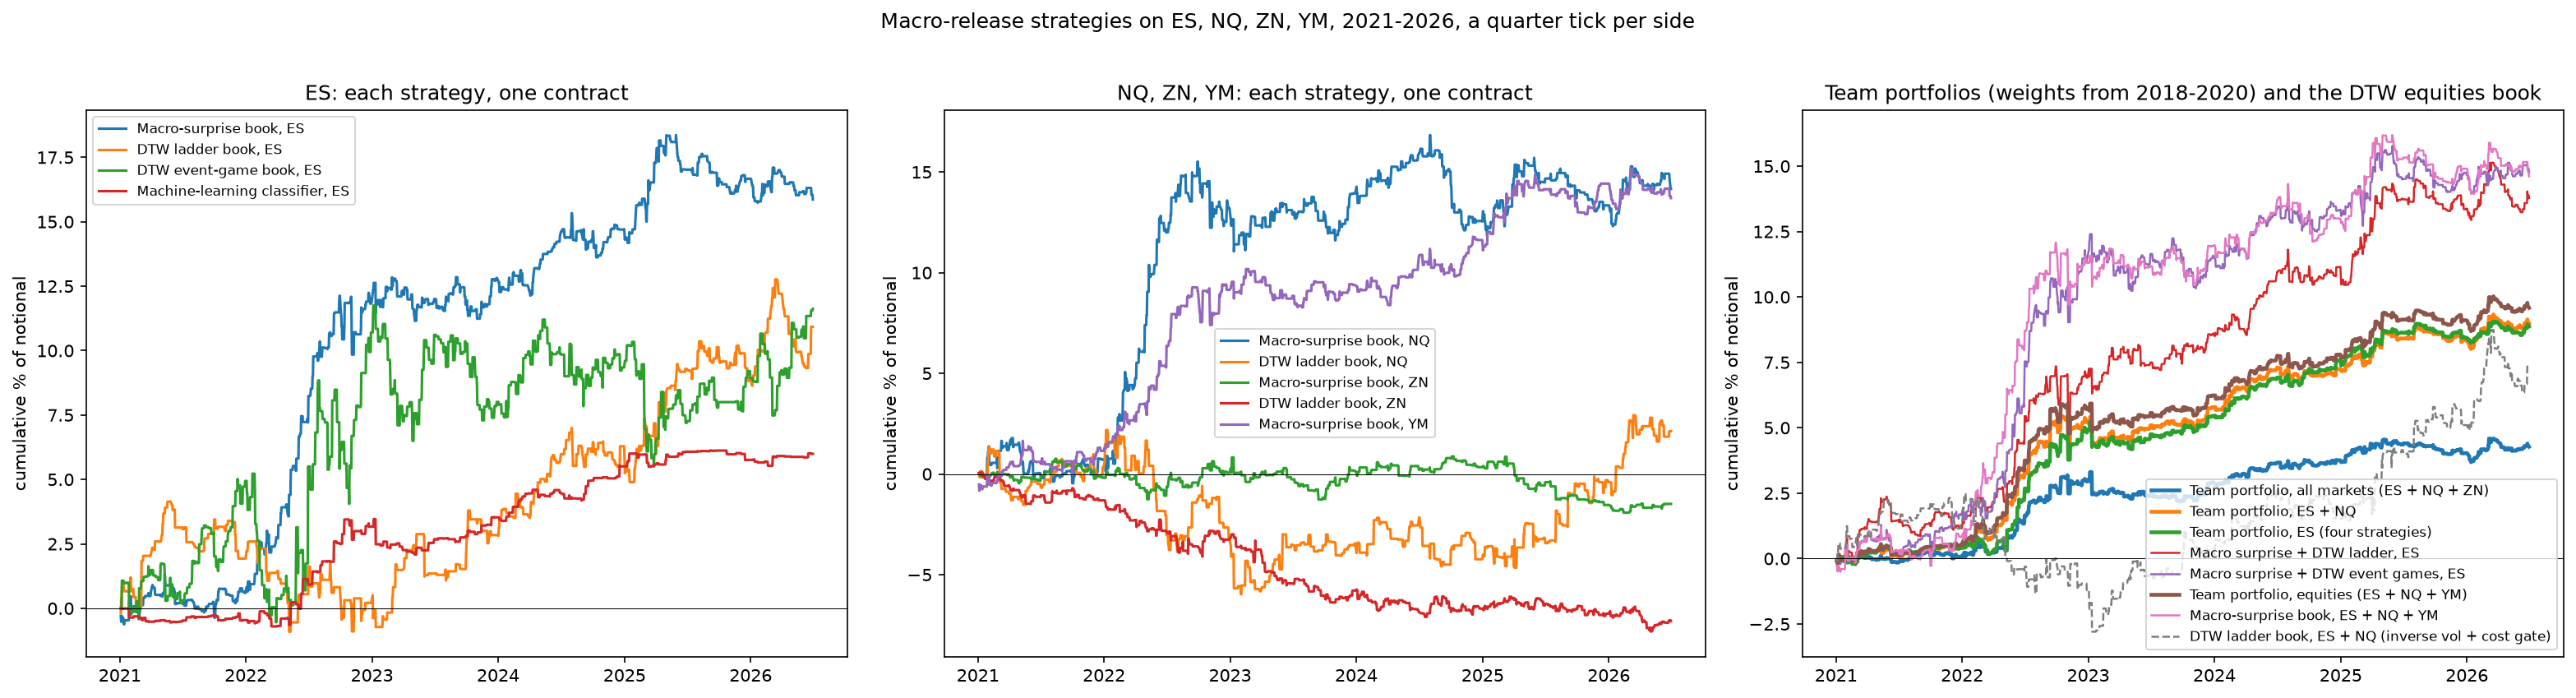
\includegraphics[width=\linewidth]{team_report_figure}
  \caption{Cumulative net P\&L at a quarter tick per side, 2021--2026: each approach in \ES\
  (left), in \NQ, \ZN\ and \YM\ (center), and the team portfolios with the DTW ladder's own
  \ES\ + \NQ\ book (right).}
  \label{fig:team}
\end{figure}

\section{Interpretation}\label{sec:mechanisms}

\subsection{Why equities and not Treasuries: tick size as a limit to arbitrage}

The surprise explains the first-minute response of \ZN\ as well as that of the equity indices, so
the absence of a tradeable drift in \ZN\ is not a failure of the signal. Two features of the
Treasury market explain it. First, a CPI or payrolls surprise maps into the expected policy path,
and hence into Treasury yields, almost mechanically, and the Treasury futures market is where the
fastest participants price that information. By the time a position can be opened, the move is
largely complete: the drift per standard deviation of the CPI signal is 0.8 bps in \ZN, against
about 6 bps in \ES\ and 8.5 bps in \NQ. For equities, investors must also judge the effect of the same number on
growth, margins and risk premia, and the drift is largest in \NQ, whose value depends most on
long-dated cash flows; \YM, with more industrial and financial stocks, reacts about 8\% less than
\ES\ but drifts by the same amount after the first minute. Second, even where a gross edge exists, one \ZN\ tick is large relative to
the post-release move: the naive CPI rule earns 2.7 bps per trade before costs and pays 3.0 bps to
trade, and the DTW ladder's gross Sharpe ratio of 0.34 becomes $-0.97$ at a quarter tick per side.
The minimum price increment thus acts as a limit to arbitrage that leaves a small predictable
component in prices unexploited.

\subsection{Why price-path analogues fail on direction}

Analogue forecasts assume that the mapping from recent price shapes to subsequent returns is
stable. Around macro releases it was not. The analogues' direction forecast had a negative rank
correlation with subsequent returns in 2013--2017 and a positive one in 2018--2020, and the
single-window analogue book that earned money in 2018--2020 lost money in \ES\ and \NQ\ in
2021--2026; on \YM, added later, it earned little in either period. Across 567 constructions of the analogue forecast (waiting times, path
lengths and neighbour weights) the training and validation correlations are almost unrelated
(correlation 0.07 across settings). The change coincides with the shift of the macro regime from
low inflation to the 2021--2022 inflation shock, when the same price shape could precede
continuation or reversal depending on how the market read the Federal Reserve's response. What the
analogues do capture is uncertainty: when similar past paths were followed by very different
outcomes, the next move tends to be large. This is why their dispersion is a stable forecast of
the size of the move and a useful input for position sizing, while their direction is not.

\subsection{What the entry assumption reveals about the speed of price discovery}

The classifier result in Table~\ref{tab:equalcosts} quantifies how much of the forecastable
component of returns is priced within the first minute. Moving the entry by one minute removes
about 80\% of the gross profit of a model that combines surprise and price information. Together
with the event-study evidence that roughly a quarter of the CPI response remains after the first
minute in equity futures, this places most of the price discovery within the first minute and a
small, economically meaningful residual in the following half hour. The residual is predictable
from public information, persists for about 30 minutes---a second 30-minute window after the release
earns negative returns in every market---and is concentrated in periods when macro data drive
expectations of monetary policy.

\section{Robustness}\label{sec:robust}

\subsection{Dependence on 2022}

The CPI strategy earned most of its profit in 2022, when inflation dominated markets and every CPI
print moved the expected path of the policy rate (Figure~\ref{fig:byyear}): 79\% of its net P\&L
in \ES\ and 74\% in \NQ. Excluding 2022, its Sharpe ratio falls from 1.03 to 0.58 in \ES\ and from 1.00
to 0.68 in \NQ\ for the naive rule. \YM\ repeats the pattern: 2022 contributes 4.1 of its 6.8
percentage points, and its Sharpe ratio excluding 2022 is about 0.5. The broad book, which spreads its risk over about ten releases,
is less concentrated: its Sharpe ratio excluding 2022 is 0.28 in \ES, 0.44 in \NQ\ and 0.40 in \YM, and the
surprise books are positive in both the validation and the test years of the equal-terms
comparison. We read the result as state dependence at the level of the macro regime: the drift is
largest when macro data drive policy expectations.

\begin{figure}[htbp]
  \centering
  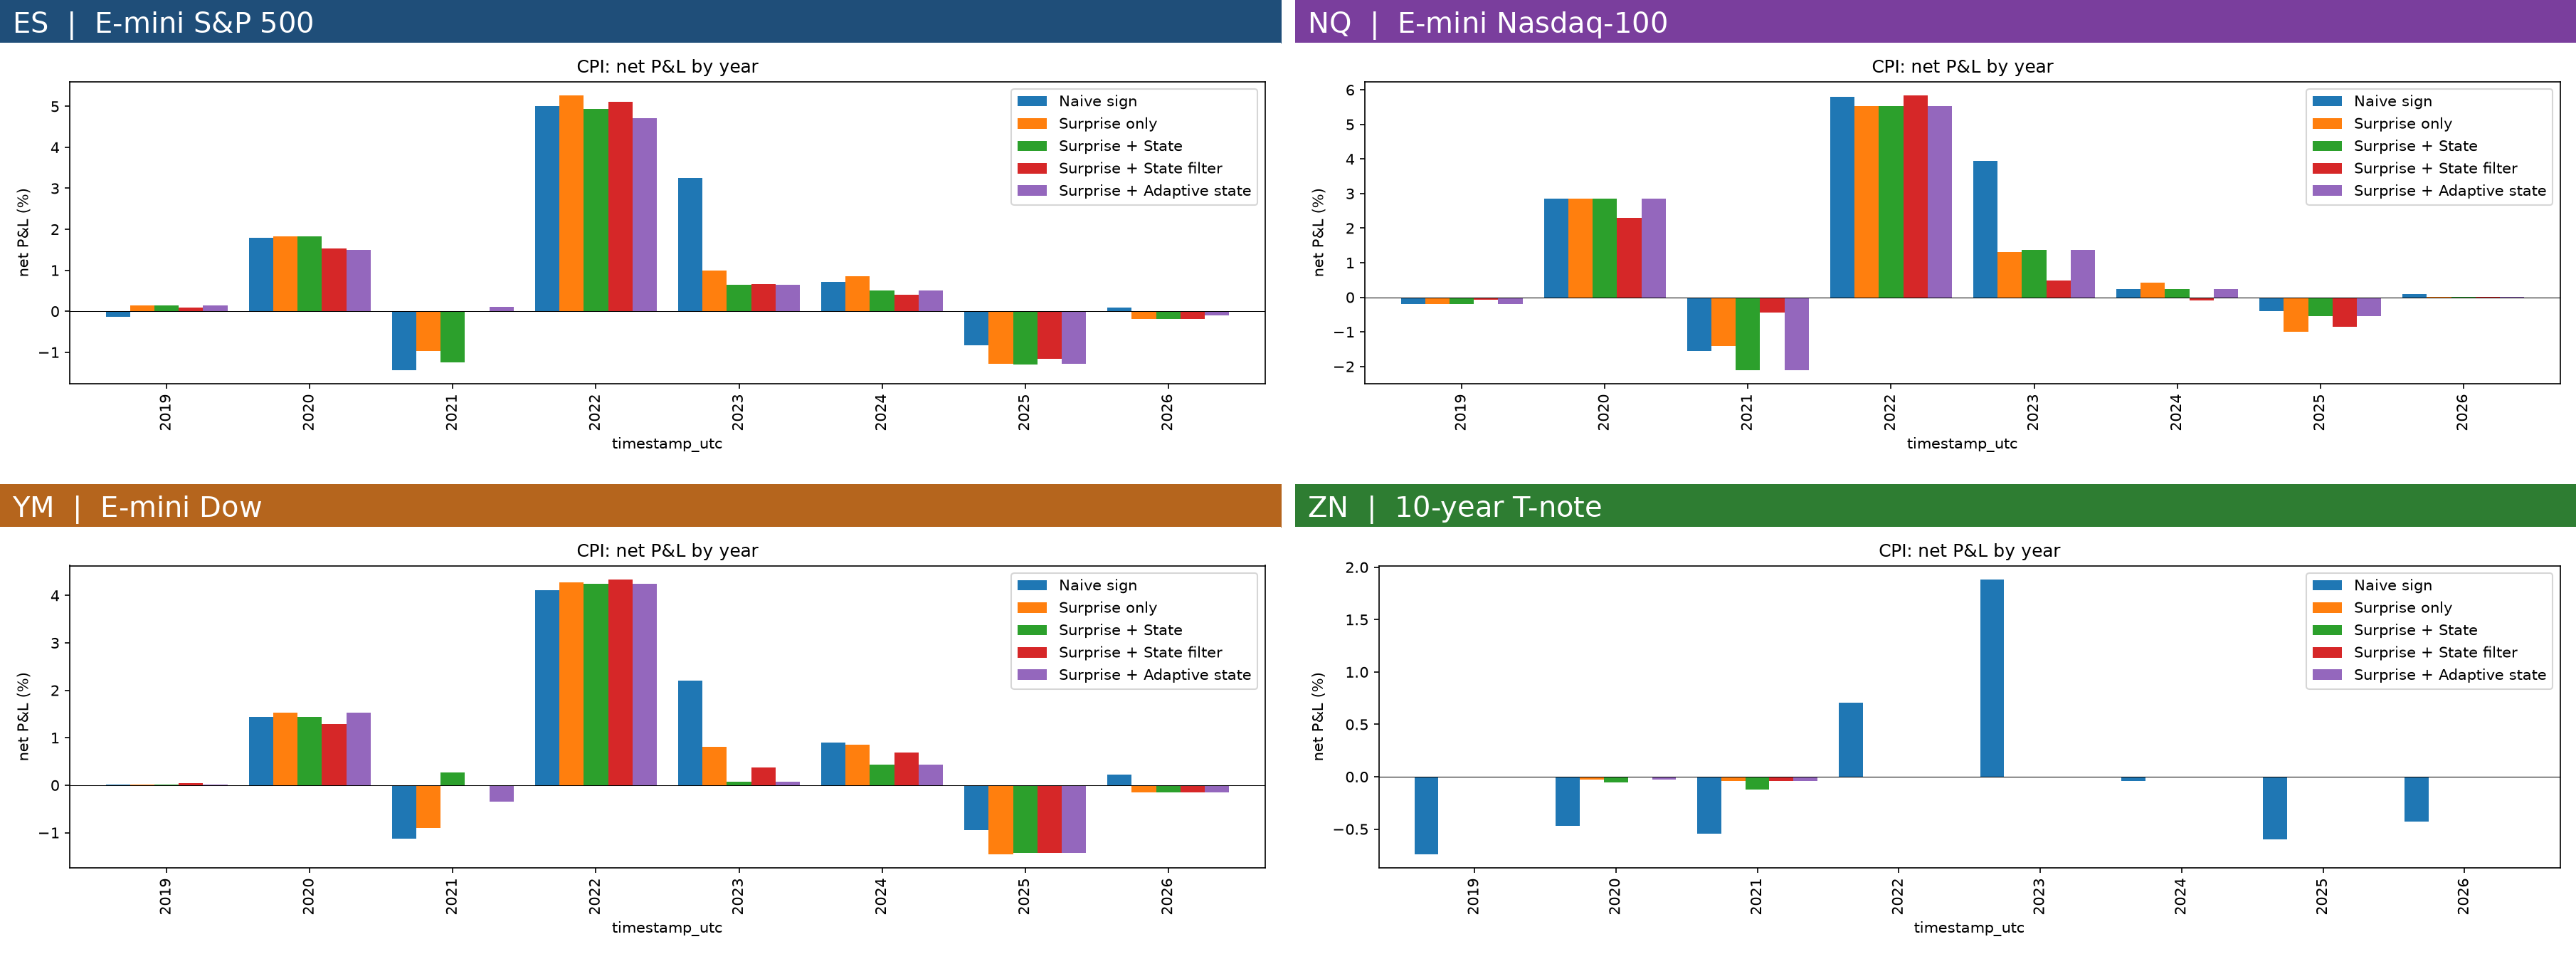
\includegraphics[width=\linewidth]{fig18_cpi_pnl_by_year_4markets}
  \caption{Net P\&L of the CPI strategies by calendar year (\% of notional), \ES, \NQ, \YM\ and \ZN.}
  \label{fig:byyear}
\end{figure}

\subsection{Entry delay and holding period}

The \ES\ CPI Sharpe ratio remains between 0.55 and 0.71 when the entry is delayed by one, two or five
minutes with a 30-minute hold, and between 0.51 and 0.62 in \NQ. \YM\ is more sensitive to the
delay: from 0.84 with no delay to 0.54, 0.33 and 0.17 after one, two and five minutes. Short holds are fragile: a
five-minute hold loses most of its Sharpe ratio when the entry is delayed by one minute. The edge is a
slow continuation over about half an hour, not a fast reaction.

\subsection{More windows per release}

A natural way to trade more often is to trade several consecutive windows after each release.
Figure~\ref{fig:ladder} shows that only the first window is clearly profitable, and mainly for the
surprise: the surprise's rank correlation with the return falls from 0.139 in the first 30 minutes
in \ES\ (0.088 in \NQ\ and 0.091 in \YM) to between $-0.06$ and $+0.05$ in the next four windows.
The analogues have no information in any window in \ES, \NQ\ and \ZN; in \YM\ their first window
earns 0.47 and the later ones lose. Every additional window adds turnover and cost but not profit; five-window
books lose between 29\% and 48\% of notional in \ES\ over 2019--2026, and on \YM\ the five-window
surprise and DTW books have Sharpe ratios of $-0.34$ and $-0.23$.

\begin{figure}[htbp]
  \centering
  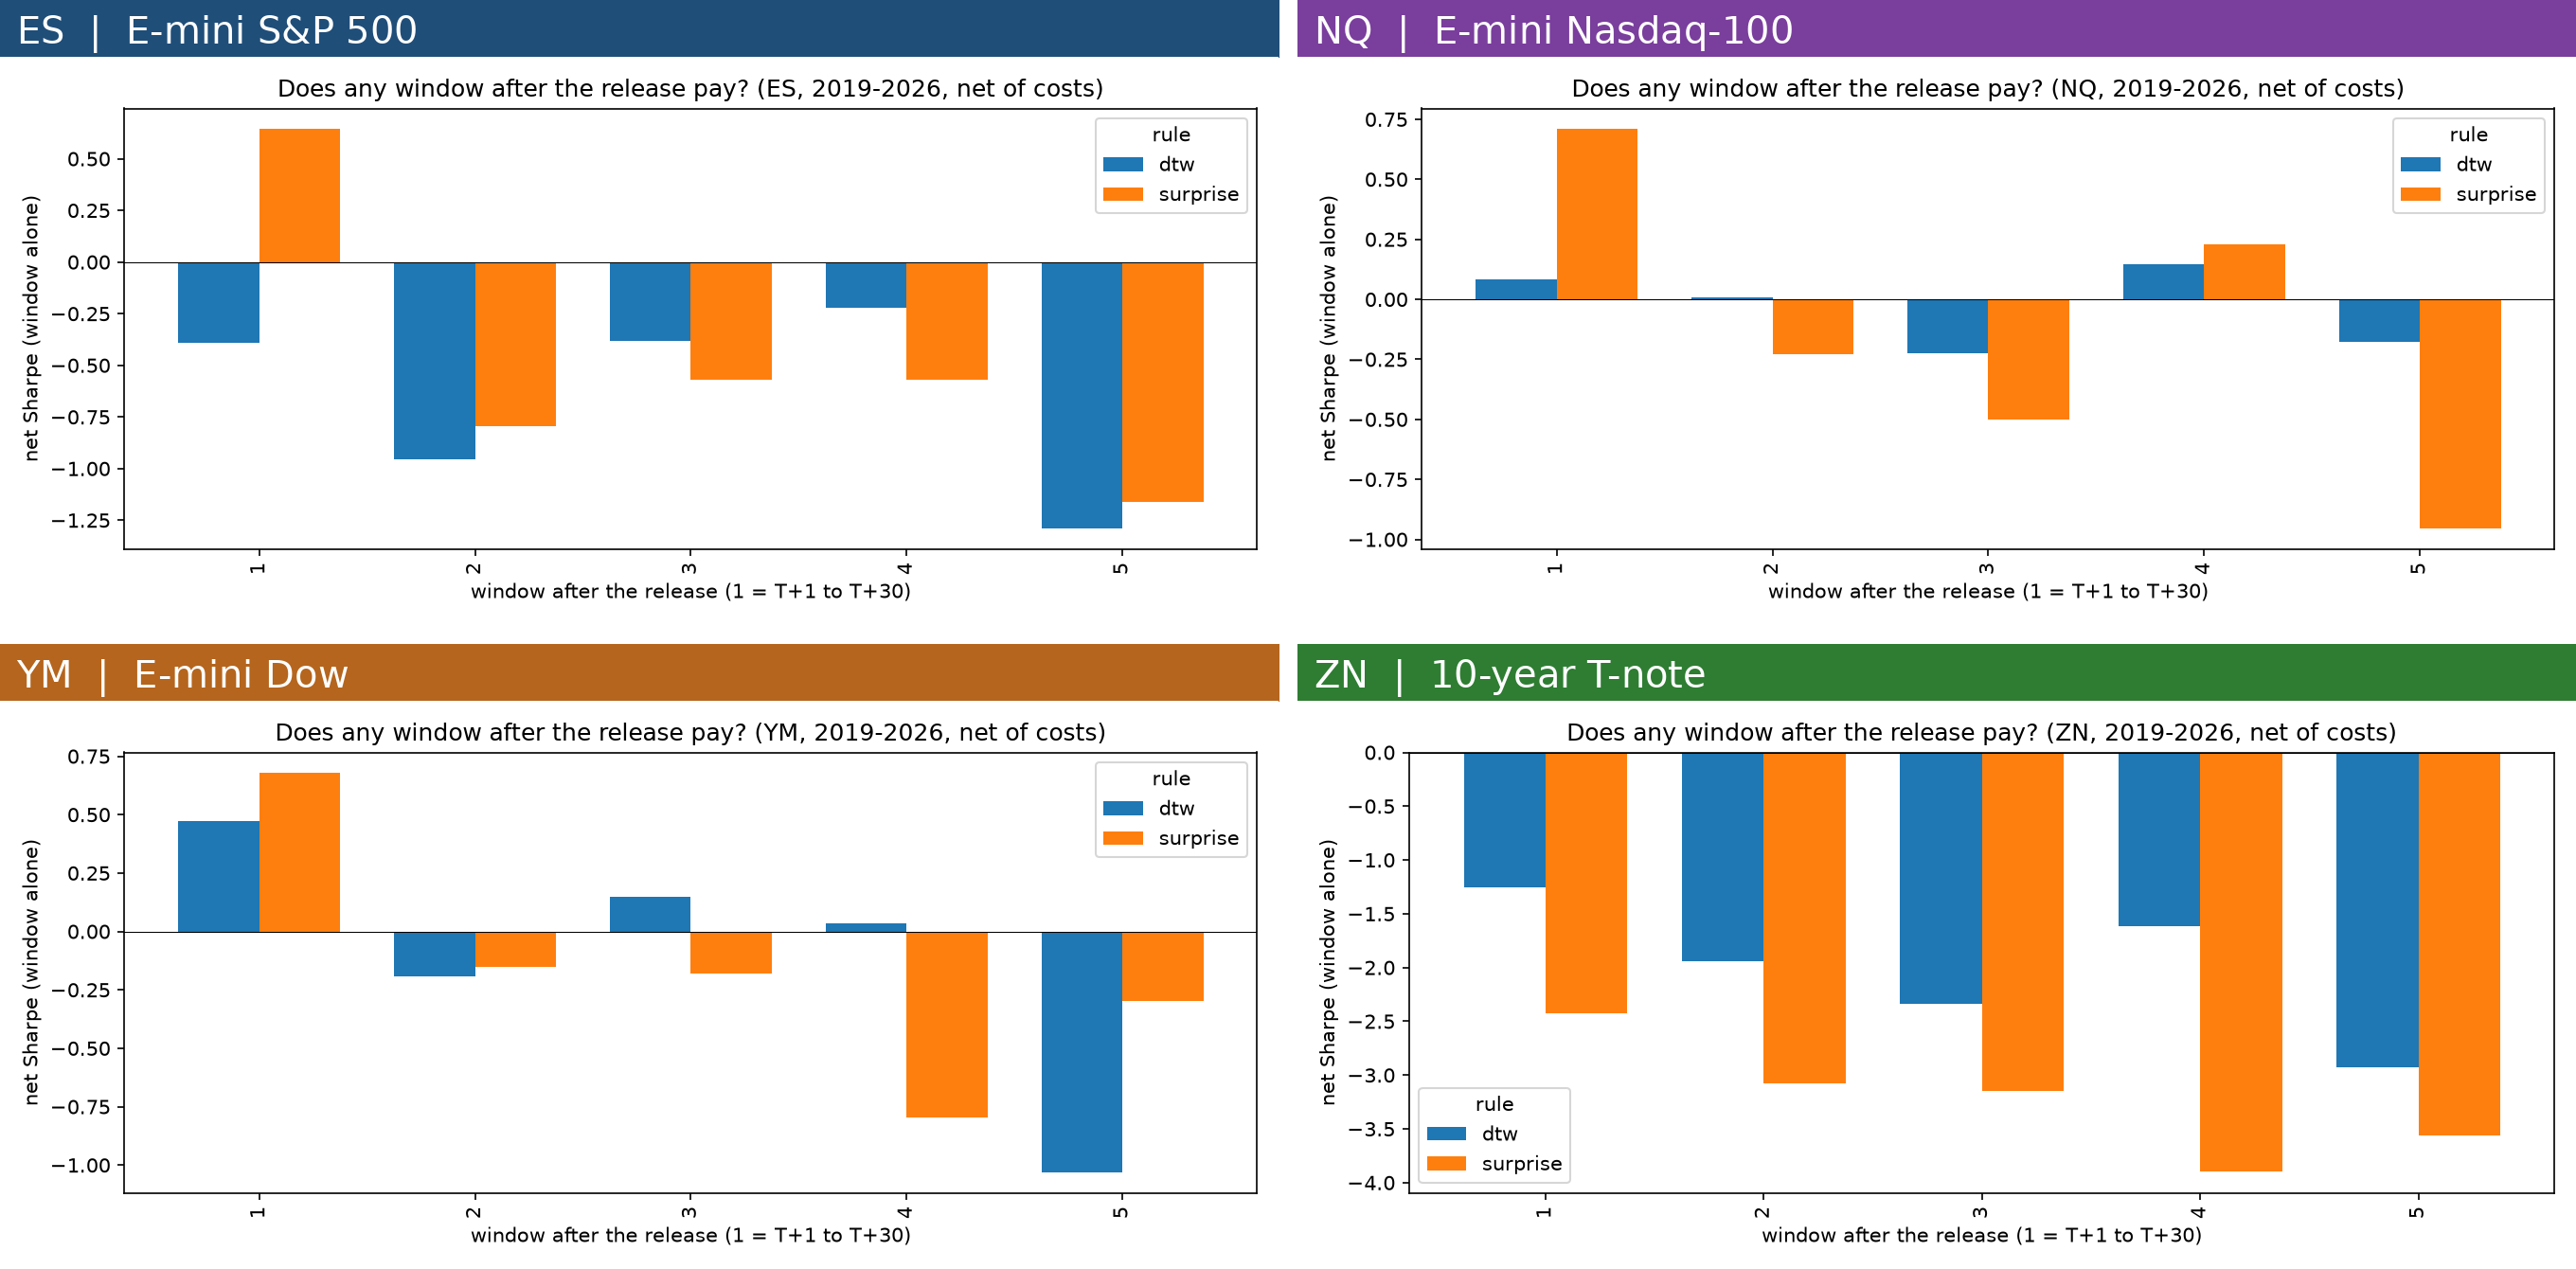
\includegraphics[width=\linewidth]{fig28_ladder_sharpe_by_window_4markets}
  \caption{Net Sharpe ratio of the surprise and DTW signals traded in each of the five 30-minute
  windows after a release, \ES, \NQ, \YM\ and \ZN, 2019--2026.}
  \label{fig:ladder}
\end{figure}

\subsection{Construction choices and multiple testing}

Pattern-based results are sensitive to reasonable construction choices. For the \ES\ DTW ladder,
the Sharpe ratio on 2021--2026 at a quarter tick ranges from 0.17 to 0.64 across the number of
neighbours, the width of the trading gate and whether its thresholds are fixed or re-estimated;
across 63 variations of waiting time, path length and neighbour weights, it ranges from $-0.45$ to
0.61. The original implementation of the ladder, with its own family grouping and data, reaches
0.64 in \ES\ on 2021--2026 at a quarter tick (random-sign $p=0.04$) but 0.11 in \NQ, and its
direction forecast has a negative rank correlation with returns in the training years. The best of
many such variations overstates what an investor could expect
\citep{Harvey2016, Bailey2014}. The surprise approach has few free choices, and its main
constants were fixed before the test years were scored. The pattern-based books also pass a leak
test: extending the price path five minutes past the entry raises the \ES\ DTW Sharpe ratio from
0.64 to 2.86, so the timing of the real book is correct and the information is not coming from
the future. In the state-dependence analysis, analytic HC3 and permutation $p$-values agree closely,
and we report only effects that survive the false-discovery correction of \citet{Benjamini1995}.

\subsection{Limitations}

Our results are subject to five limitations. First, costs are modeled rather than observed; fills
in the first minute after a release may be worse than two ticks. Second, the sample contains about
120 releases per family, and CPI-only results rest on 50--90 trades. Third, the event-game setting was
chosen on the full sample, and the \YM\ results were produced after the \ES\ and \NQ\ results were
known, although with unchanged code and constants. Fourth, the test years have been examined more than once during the
project, so they are not an untouched hold-out for any approach. Fifth, for near-zero CPI surprises
the sign depends on which CPI line is used: the headline and the family average disagree on 20 of
86 releases, which changes the CPI Sharpe ratio from 1.03 to 0.51 in \ES.

\section{Directions for Future Research}\label{sec:future}

Our results answer one question---how much of the news is left after the first minute---and
raise several others. We group them by the finding that motivates each, and for each we say what
data or test would answer it.

\paragraph{1. Execution in the first minutes.} Every result in the paper depends on the cost
of a trade one minute after a release, and we model that cost as a fixed number of ticks. In
practice, depth in the order book thins out just before a release and rebuilds over the next
minutes, so slippage is itself state-dependent: it is likely to be largest after the largest
surprises, which are the trades the surprise model takes. Recorded fills, or depth-of-book data
(for example Databento's MBP-10 feed for the same contracts), would allow the cost in
equation~\eqref{eq:cost} to be replaced by a measured cost that depends on the size of the surprise,
the time since the release and the trade's size. The same data would answer how much capital the
strategy can carry before its own trades move the price, a question our backtests cannot address.

\paragraph{2. Price discovery inside the first minute.} We find that most of the response is in
the first minute, but our bars cannot say how it is distributed within that minute. Tick data
would show how many seconds the market needs to price a surprise, whether the speed has changed
over the sample, and whether the residual drift we trade is related to how quickly the first
seconds absorb the news. It would also allow the analysis of latency in
Section~\ref{sec:environment} to be extended from minutes to seconds, so that the value of the
first-minute jump to a faster trader can be measured rather than excluded.

\paragraph{3. Better measures of the surprise.} We measure the surprise as the actual figure minus
the median forecast, standardized. Several refinements are natural. The dispersion of forecasts
measures how uncertain the market was, and a surprise relative to an uncertain consensus may be
priced differently. Revisions to earlier releases and the components of a release (core versus
headline, services versus goods) may carry information that the headline surprise misses. Nowcasts
and market-implied expectations, such as inflation swaps or fed funds futures, are a measure of what
was expected that is less stale than a survey. Finally, the text of the release and of FOMC
statements and minutes can be scored with language models, which would bring the FOMC decision---which
our impact screen does not admit---into the event set.

\paragraph{4. Regimes and the Fed's reaction function.} The surprise book earns most of its return in
2022: without that year its Sharpe ratio is close to zero in every equity market
(Figure~\ref{fig:byyear}). A plausible explanation is that inflation surprises matter most when the
Fed is expected to respond to them. This can be tested directly by conditioning the drift on
measures of the policy regime---the expected path of rates, whether the Fed is tightening, the
level of inflation relative to target---and by letting the coefficients in
equation~\eqref{eq:drift_model} vary over time, for example with a Kalman filter or a rolling
Bayesian prior. A model of this kind would also say in advance when the edge is likely to be small,
which is as valuable to a practitioner as the edge itself.

\paragraph{5. Extensions of price-path analogues.} DTW analogues do not forecast the direction of
the drift, but their dispersion forecasts its size, the first window after the release is the best of the five, and the analogues add value when they agree with the surprise:
in \YM\ the book that trades only when the two agree has a Sharpe ratio of 0.94 with the same value
outside 2022. These findings suggest four extensions. First, multivariate paths that match the equity
and Treasury reaction together, since the joint reaction says more about the nature of the news
than either market alone. Second, a book that uses DTW only for sizing and the surprise for direction,
tested out of sample on all four markets. Third, learned similarity measures (for example shapelets or
a neural embedding of the path) in place of a fixed distance. Fourth, a book that trades only the
first window, which keeps the part of the ladder with information and drops the part that only adds
costs.

\paragraph{6. Other markets and countries.} The tick-size explanation for the Treasury result
predicts that a contract with a finer tick relative to its moves should show a tradable drift. This
can be tested on the 2-year and 5-year notes and on SOFR futures, whose ticks are small relative to
their moves around policy news, and on the Bund, the gilt and JGB futures around their own countries'
releases. In equities, the Russell 2000 future (traded since 2017) and the Euro Stoxx 50 offer a
test of whether the drift is larger in less liquid or more rate-sensitive indices. Currency and
commodity futures around U.S.\ releases would show whether the drift is a feature of U.S.\ equity
futures or of how markets in general absorb scheduled news.

\paragraph{7. Portfolio construction.} Our portfolios use fixed equal-risk weights, chosen on
2016--2018. The approaches lose in different years, which suggests that weights that adapt---to recent
performance, to the regime of item 4, or to the expected cost of item 1---could do better, though at
the price of more choices and a higher risk of overfitting. A careful test would fix the rule for
changing the weights in advance and report it with the same random-sign and walk-forward checks we
use for the books themselves.

\paragraph{8. Why does the drift exist?} We document a drift but test its cause only indirectly.
Three explanations make different predictions. Limits to arbitrage predict a larger drift when
liquidity is thin and costs are high. Limited attention predicts a larger drift when several releases
arrive at the same time or when the surprise is in a less-watched component. Disagreement predicts a
larger drift when forecasts are dispersed and when volume after the release is high. Volume, order-flow
imbalance and the dispersion of forecasts around each release are enough to tell them apart, and the
answer would say whether the edge is likely to last.

\section{Conclusion}\label{sec:conclusion}

How much of the macroeconomic news is left after the first minute? In equity-index futures, about
a quarter of the response to a CPI surprise arrives after the first minute, the consensus surprise
predicts its direction out of sample, and the drift lasts about 30 minutes. A strategy that trades
it one minute after the release earns a Sharpe ratio of about 0.7--1.1 in \ES, \NQ\ and \YM\ depending on
the set of releases and the cost assumption, with no exposure to the market. Combined with the
other approaches, which lose in different years, the equity-index portfolio reaches 1.35 at a
quarter tick and 0.85 at our base cost. In Treasury futures,
the surprise is priced just as reliably, but almost entirely within the first minute, and the
remaining drift is smaller than one tick. Price-path analogues do not forecast the direction of
the drift, although their dispersion forecasts its size, and backtests that enter at the release
price attribute to skill a first-minute jump that no investor can trade.

These results have implications for both research and practice. They place most of the price
discovery after scheduled releases within the first minute, identify the minimum tick as a
friction that leaves a small predictable component in Treasury prices, and show that the evaluation
of event-driven strategies must fix the entry at an executable price. For practitioners, the
consensus surprise is the source of a small but persistent edge in equity-index futures, the
dispersion of price-path analogues is a useful risk input, and execution quality in the first
minute after a release decides whether the edge survives. Section~\ref{sec:future} sets out the
research that would test these conclusions further, from measured execution costs and tick data to
richer surprise measures and other markets.


\clearpage
\IfFileExists{aea.bst}{\bibliographystyle{aea}}{%
  \IfFileExists{chicago.bst}{\bibliographystyle{chicago}}{\bibliographystyle{apalike}}}
\bibliography{references}

\clearpage
\appendix
\renewcommand{\thesection}{Appendix \Alph{section}}
\setcounter{figure}{0}\setcounter{table}{0}
\renewcommand{\thefigure}{A\arabic{figure}}
\renewcommand{\thetable}{A\arabic{table}}
% In-paper appendix: essential technical material only (counts toward AER page length).
\section{Surprise Construction}\label{app:surprise}

\paragraph{Release families.} Two release lines belong to the same family if the share of the
larger line's release timestamps that are shared by both is at least 80\%; families are formed
transitively (union-find). The family is named after its best-known line (e.g.\ ``CPI'').
Families need at least 30 releases to be traded.

\paragraph{Standardization.} For each line, $z_{l,t}$ in equation~\eqref{eq:z} uses the standard
deviation of the line's earlier raw surprises only, requires at least 24 of them and is capped at
$\pm5$. Releases are de-duplicated by line and timestamp, keeping the last revision.

\paragraph{Signs and screen.} For each market and year, the sign $s_l$ is the sign of the OLS
slope of the first-minute return on $z_{l,t}$ over earlier years (at least 24 observations). The
impact screen ranks families by the ratio of their mean absolute 30-minute reaction to the same
statistic at the same clock time on other families' releases, over earlier years, and admits the
top ten, plus CPI.

\section{Dynamic Time Warping Forecast}\label{app:dtw}

For a query path $q$ and a candidate path $c$, both z-scored and of length $n$, the DTW distance is
\[
  d(q,c) = \min_{\pi\in\mathcal{P}_w} \sum_{(i,j)\in\pi} (q_i - c_j)^2 ,
\]
where $\mathcal{P}_w$ is the set of monotone alignment paths that stay within a Sakoe--Chiba band
of $w$ minutes of the diagonal \citep{Sakoe1978}. Candidates are earlier releases at the same clock
time whose trade had closed before the current entry, within a three-year lookback and at most the
600 most recent. For the $k$ nearest candidates with distances $d_j$, ages $a_j$ (years) and
subsequent 30-minute returns $y_j$, the weights are $\omega_j \propto d_j^{-1}\,2^{-a_j/2}$, the
direction forecast is $\mu=\sum_j\omega_j y_j$ and the dispersion forecast is
$\sigma=\big(\sum_j\omega_j (y_j-\mu)^2\big)^{1/2}$. The ladder trades $\operatorname{sign}(\mu)$ when
$\mu$ lies outside the 30th--70th percentiles of its earlier values, with size
$\min\{\text{median}(\sigma)/\sigma,\,2\}$ contracts.

\clearpage
\section{Additional Figures and Tables}\label{app:additional}

This appendix collects supporting results from the project's notebooks 02--07, in the order of
the analysis: the event study (notebook 02), state dependence (03), the walk-forward CPI strategy
(04), the broad surprise book (05), surprise and DTW (06) and the multi-market book (07). Unless noted, the evaluation window is 2019--2026, the cost is two
ticks plus \$4.50 per round trip, and every estimate uses only earlier data.

\FloatBarrier
\subsection{Event study (notebook 02)}

Figure~\ref{fig:app_es_event} shows, for \ES, how large the move after CPI, payrolls and PCE is at
each horizon and how much of it the surprise explains. The move after CPI keeps growing for about
30 minutes; the share explained by the surprise is highest at one minute and stays near 0.25,
while payrolls move \ES\ almost as much but with an $R^2$ below 0.07. Figure~\ref{fig:app_es_beta}
shows the coefficient of each headline surprise by horizon: a one-standard-deviation hot CPI
print lowers \ES\ by 18 bps after one minute and by about 24 bps after 30 minutes. Table~\ref{tab:app_impact}
reports the mean absolute move in all four markets.

\begin{figure}[!htb]
  \centering
  \begin{subfigure}[b]{0.49\linewidth}\centering
    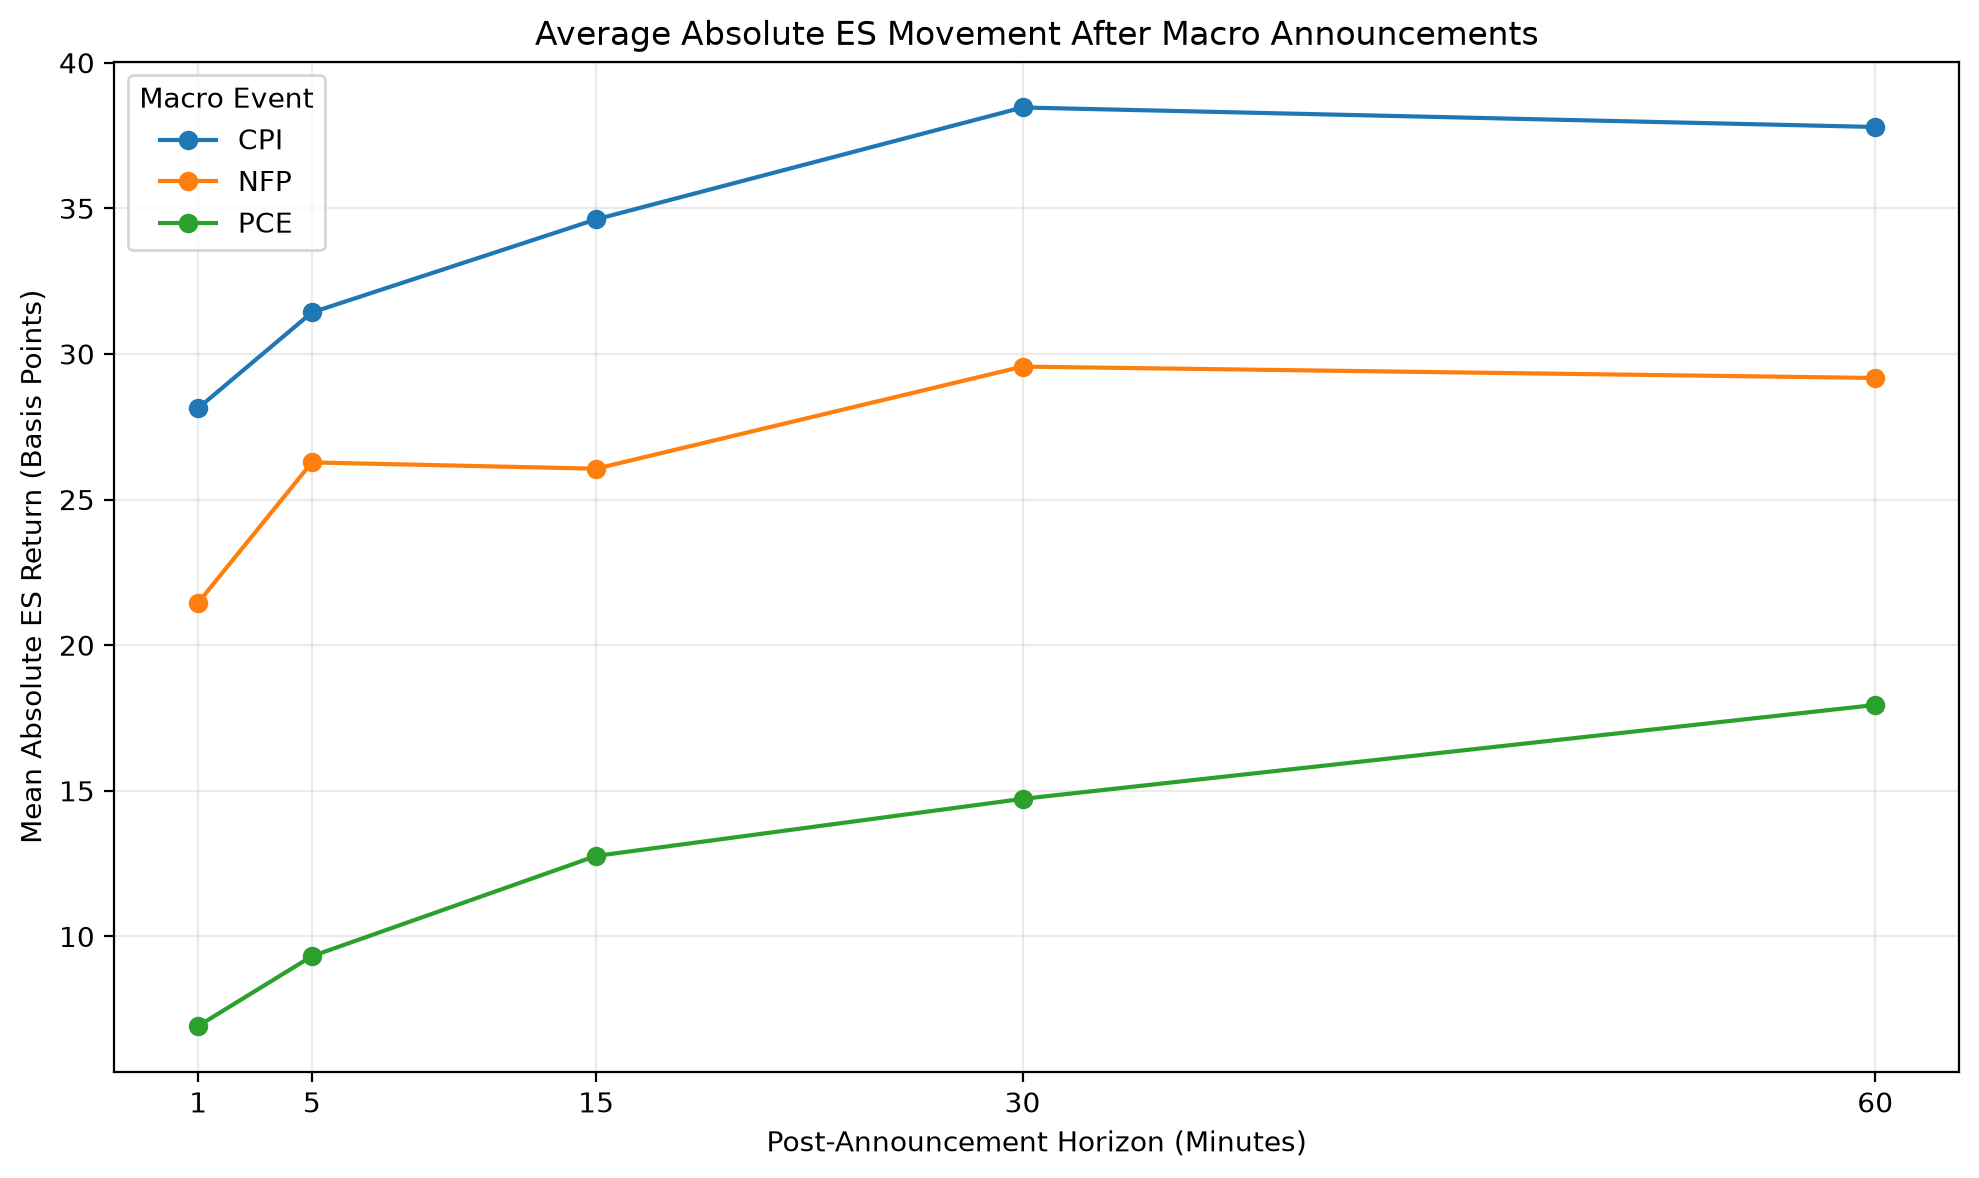
\includegraphics[width=\linewidth]{app_macro_market_impact}
    \caption{Mean absolute \ES\ return after each release.}
  \end{subfigure}\hfill
  \begin{subfigure}[b]{0.49\linewidth}\centering
    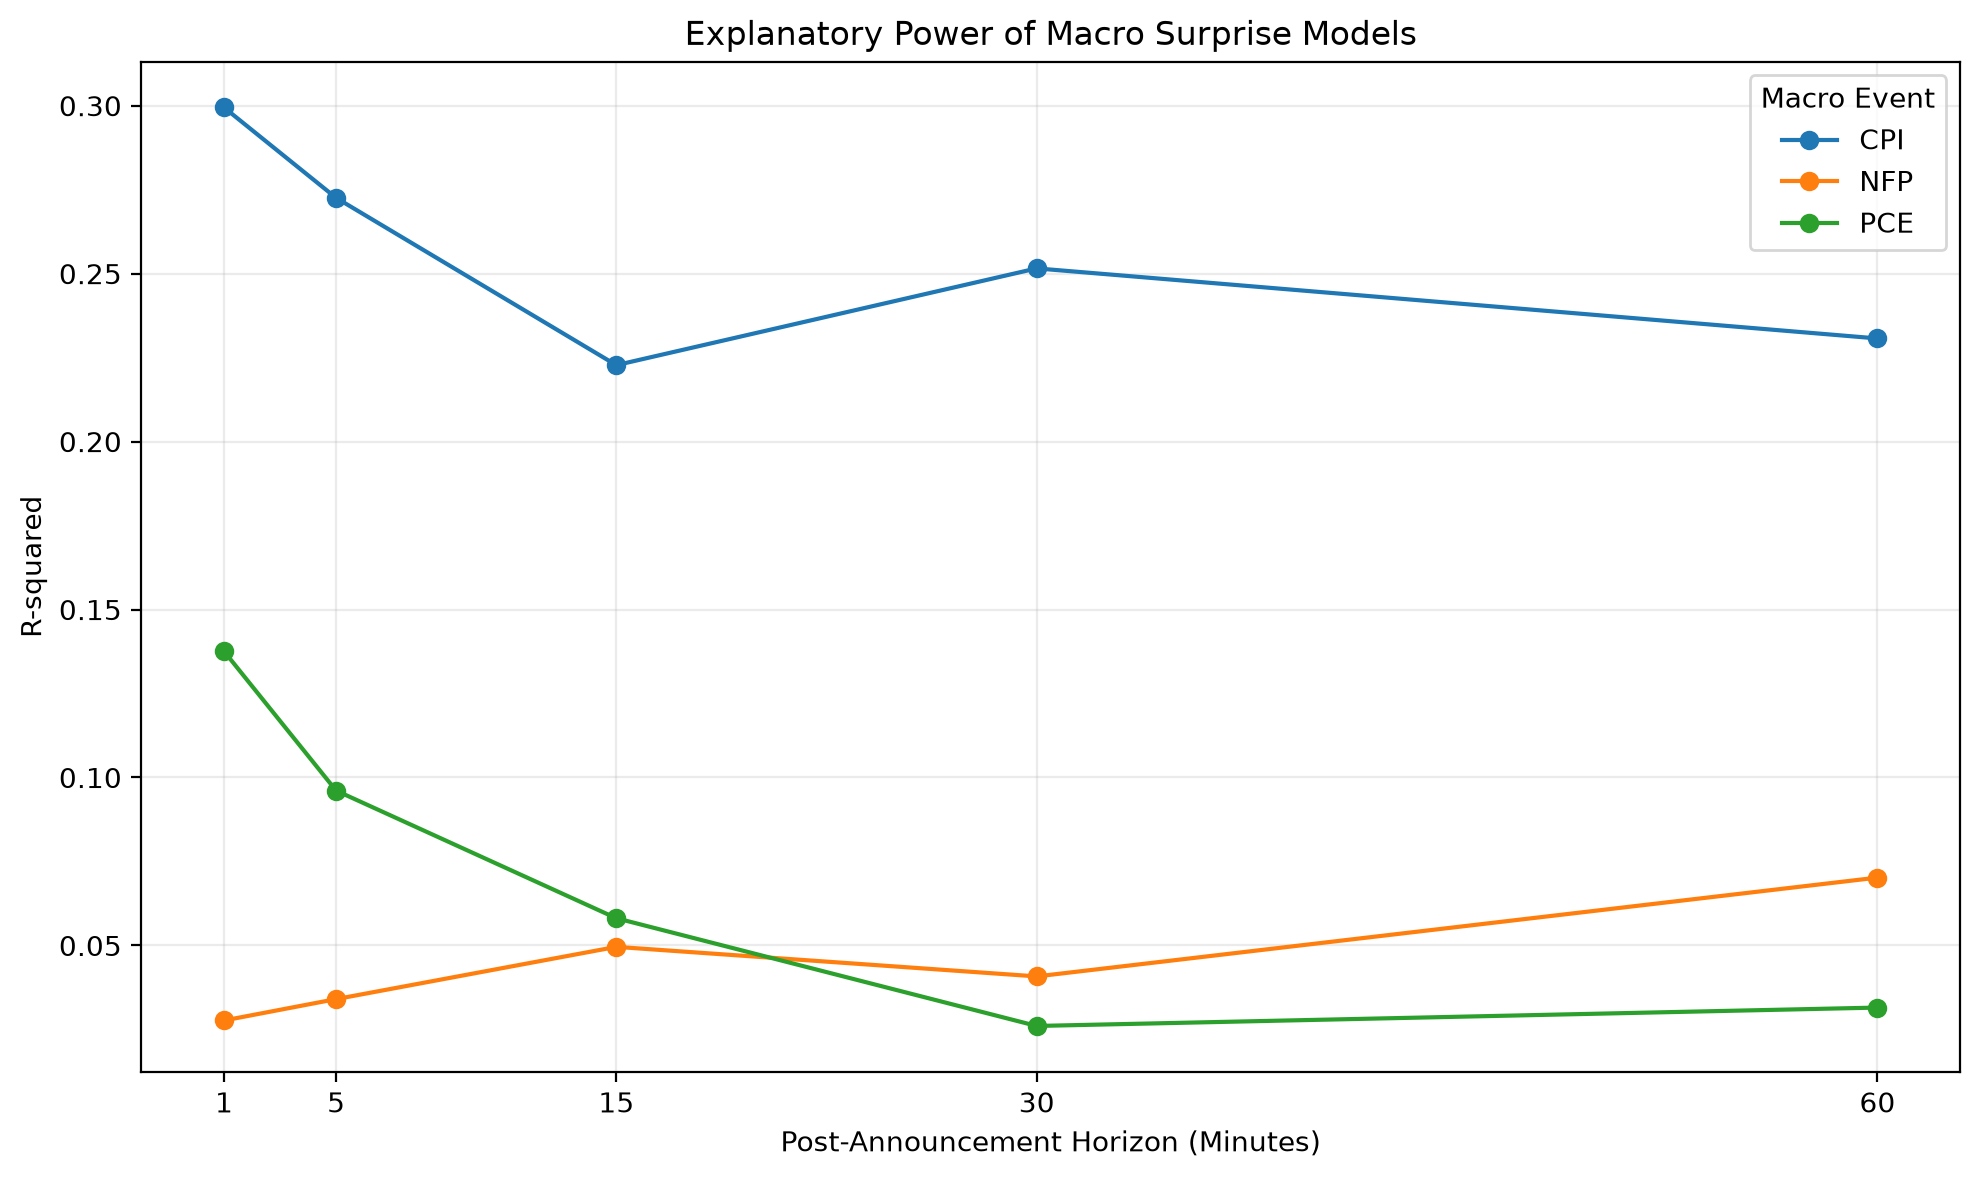
\includegraphics[width=\linewidth]{app_macro_r2_comparison}
    \caption{$R^2$ of the surprise regressions.}
  \end{subfigure}
  \caption{\ES\ after CPI, payrolls (NFP) and PCE, 2016--2026, by horizon.}
  \label{fig:app_es_event}
\end{figure}

\begin{figure}[!htb]
  \centering
  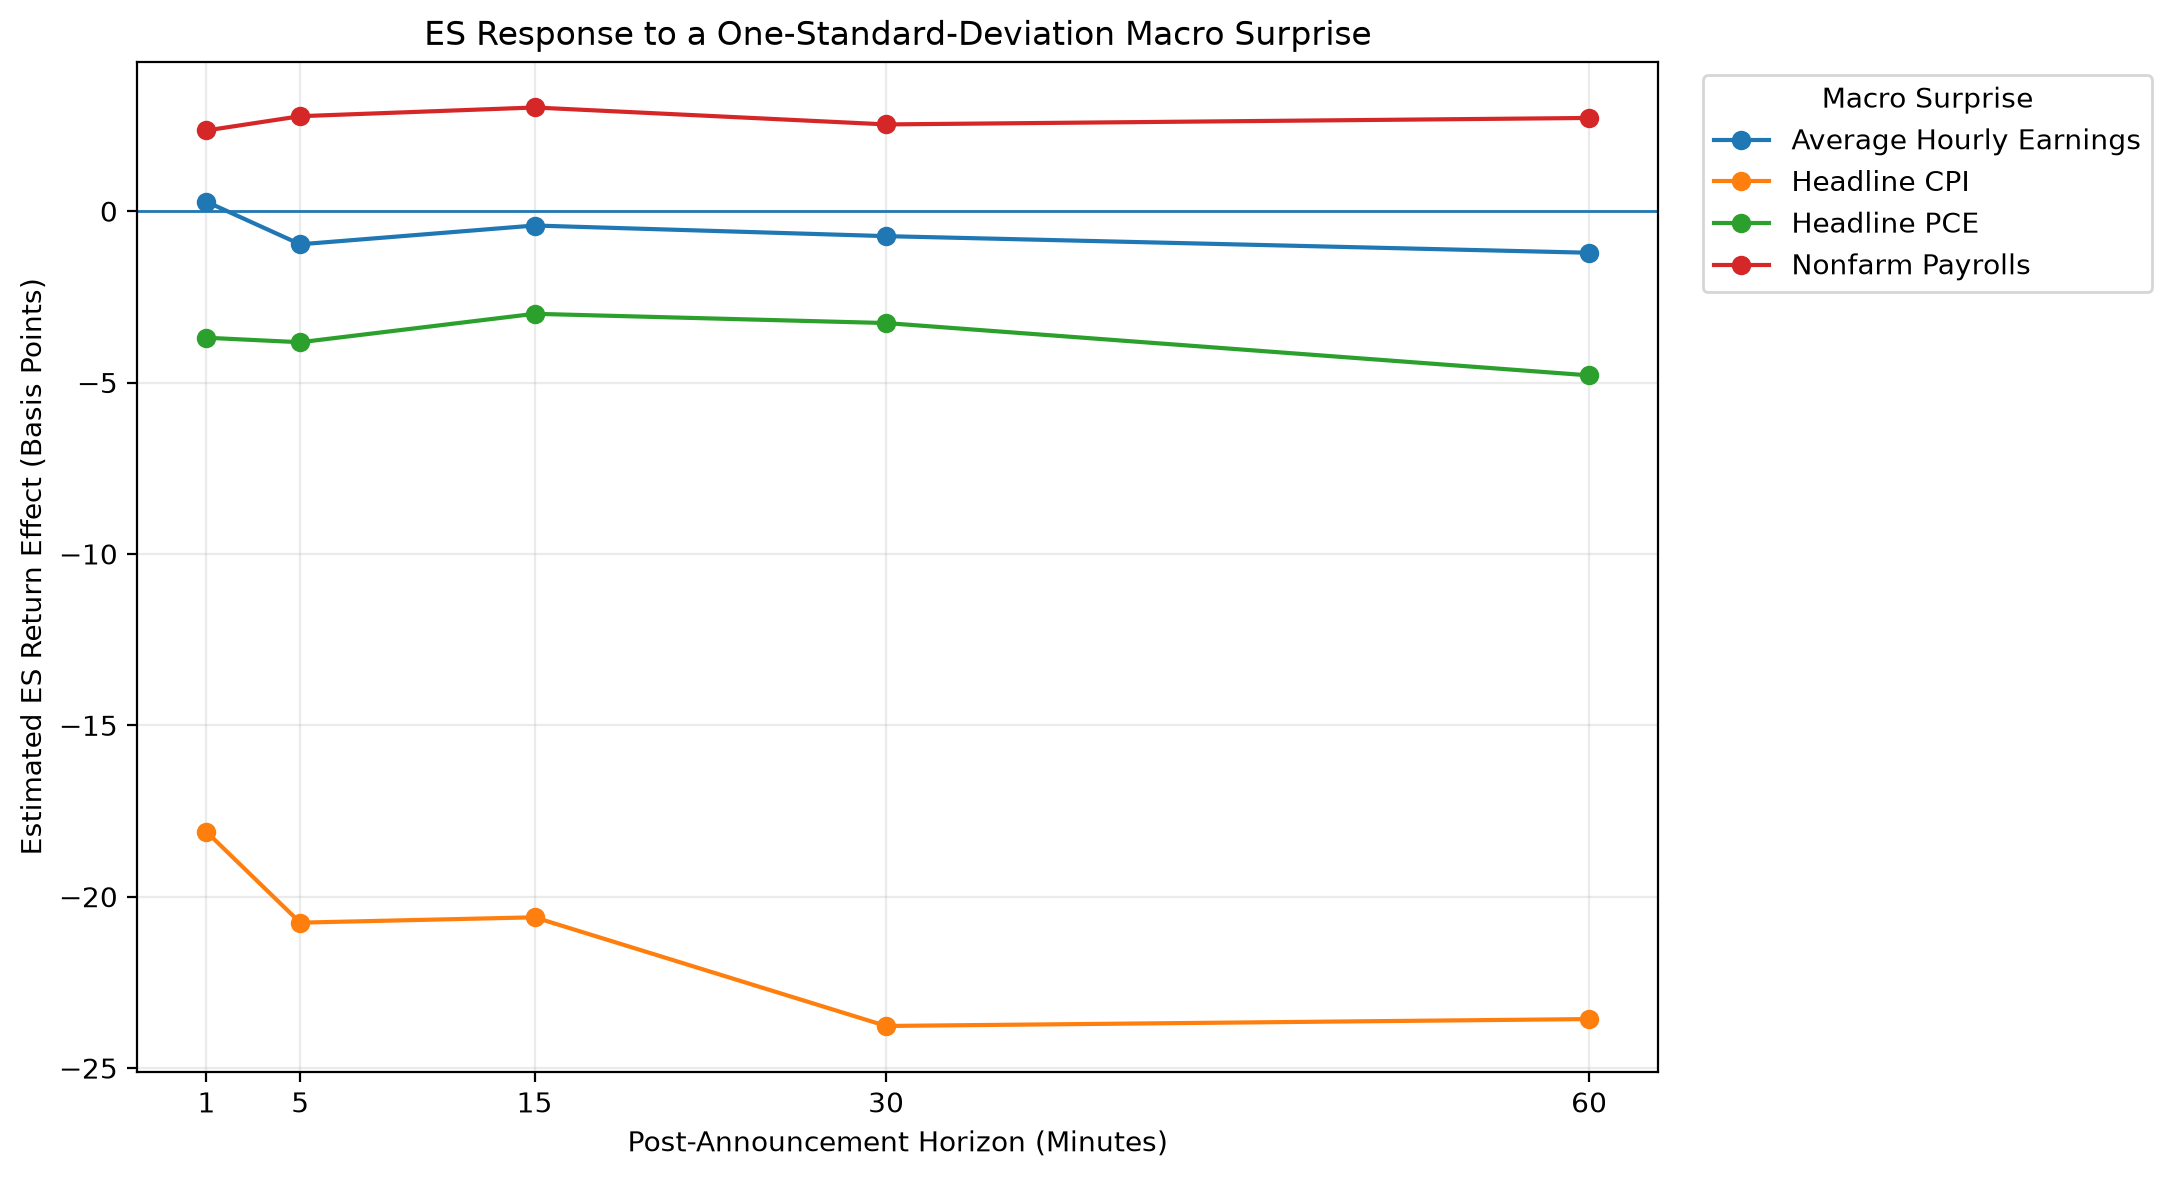
\includegraphics[width=0.62\linewidth]{app_macro_surprise_coefficients}
  \caption{\ES\ response to a one-standard-deviation surprise in each headline statistic, by
  horizon (bps), from regressions on all surprise components of the release.}
  \label{fig:app_es_beta}
\end{figure}

\begin{table}[!htb]
  \centering\small
  \caption{Mean absolute return after the release (bps), 2016--2026.}\label{tab:app_impact}
  \begin{tabular}{llccccc}
    \toprule
    Market & Release & 1 min & 5 min & 15 min & 30 min & 60 min \\
    \midrule
    \ES & CPI & 28.1 & 31.4 & 34.6 & 38.5 & 37.8 \\
        & NFP & 21.5 & 26.3 & 26.1 & 29.6 & 29.2 \\
        & PCE &  7.0 &  9.4 & 12.9 & 14.9 & 18.1 \\
    \NQ & CPI & 38.6 & 44.7 & 48.4 & 53.6 & 54.0 \\
        & NFP & 25.6 & 31.6 & 31.5 & 36.0 & 35.1 \\
        & PCE &  9.2 & 12.5 & 17.2 & 18.5 & 23.2 \\
    \YM & CPI & 23.7 & 27.7 & 29.6 & 33.2 & 33.3 \\
        & NFP & 19.3 & 23.7 & 25.0 & 27.9 & 28.6 \\
        & PCE &  5.4 &  7.3 & 10.2 & 11.9 & 15.9 \\
    \ZN & CPI & 18.4 & 20.2 & 21.4 & 22.5 & 24.0 \\
        & NFP & 20.0 & 21.6 & 22.2 & 23.6 & 24.4 \\
        & PCE &  4.9 &  6.1 &  7.3 &  8.3 &  9.3 \\
    \bottomrule
  \end{tabular}
\end{table}

\FloatBarrier
\subsection{State dependence (notebook 03)}

Table~\ref{tab:app_states} lists the six pre-registered state variables, all measured before the
release, with the hypothesis each was chosen to test. Four further variables are reported in the
figures but were not used to select models: 5-day momentum, the gap to the 50-day moving average,
realized volatility over the last 60 minutes, and the return over the last 60 minutes.

\begin{table}[!htb]
  \centering\small
  \caption{Pre-registered state variables and hypotheses.}\label{tab:app_states}
  \begin{tabular}{p{0.15\linewidth}p{0.36\linewidth}p{0.41\linewidth}}
    \toprule
    State & Definition (known before $T$) & Hypothesis \\
    \midrule
    \texttt{rv\_20d} & 20-day realized volatility of daily closes (annualized \%) & High-volatility regimes give a larger surprise beta (uncertainty, thinner liquidity) \\
    \texttt{rv\_pre\_1d} & Realized volatility of 5-minute returns over the last $\sim$23 trading hours (bps) & Short-term stress amplifies the reaction \\
    \texttt{mom\_20d} & 20-day log return (\%) & After strong rallies, bad news hits harder (stretched positioning) \\
    \texttt{dd\_60d} & Distance from the 60-day high (\%) & In drawdowns the market is more sensitive to inflation news \\
    \texttt{overnight\_ret} & Return from the prior 16:00 ET close to $T-1$ (bps) & A large pre-release move signals partial pre-positioning, so less is left to react \\
    \texttt{prev\_x} & Previous signed surprise of the same family & Surprise streaks: a second hot print confirms the trend, so the response is larger \\
    \bottomrule
  \end{tabular}
  \par\smallskip\footnotesize Exploratory (reported, not used for selection): \texttt{mom\_5d},
  \texttt{ma50\_gap}, \texttt{rv\_pre\_60m}, \texttt{ret\_pre\_60m}. Each state enters
  equation~\eqref{eq:state} as a percentile against its trailing one-year distribution.
\end{table}

Figure~\ref{fig:app_daily_state} shows three of the daily states in each market from 2010 to
2026, computed on roll-adjusted daily closes. The states vary a lot over the sample, so the terciles
used below compare genuinely different regimes: 20-day volatility in the equity indices is near
10\% in the quiet years before 2018 and peaks at 90--100\% in March 2020, with further spikes in
2011, 2015, 2018, 2022 and April 2025, and drawdowns from the 60-day high reach $-35$ to $-40\%$ in
2020. \ZN's states move with the rate cycle rather than with equity stress: its volatility is
elevated through 2022--2023 and its deepest drawdown ($-10\%$) is in 2022. The \ES\ volatility of
about 85\% in 2011 is overstated: the notebook computes it from the original vendor file, whose
early sessions are incomplete; \YM, from a complete file, peaks at about 45\% in the same episode.

\begin{figure}[!htb]
  \centering
  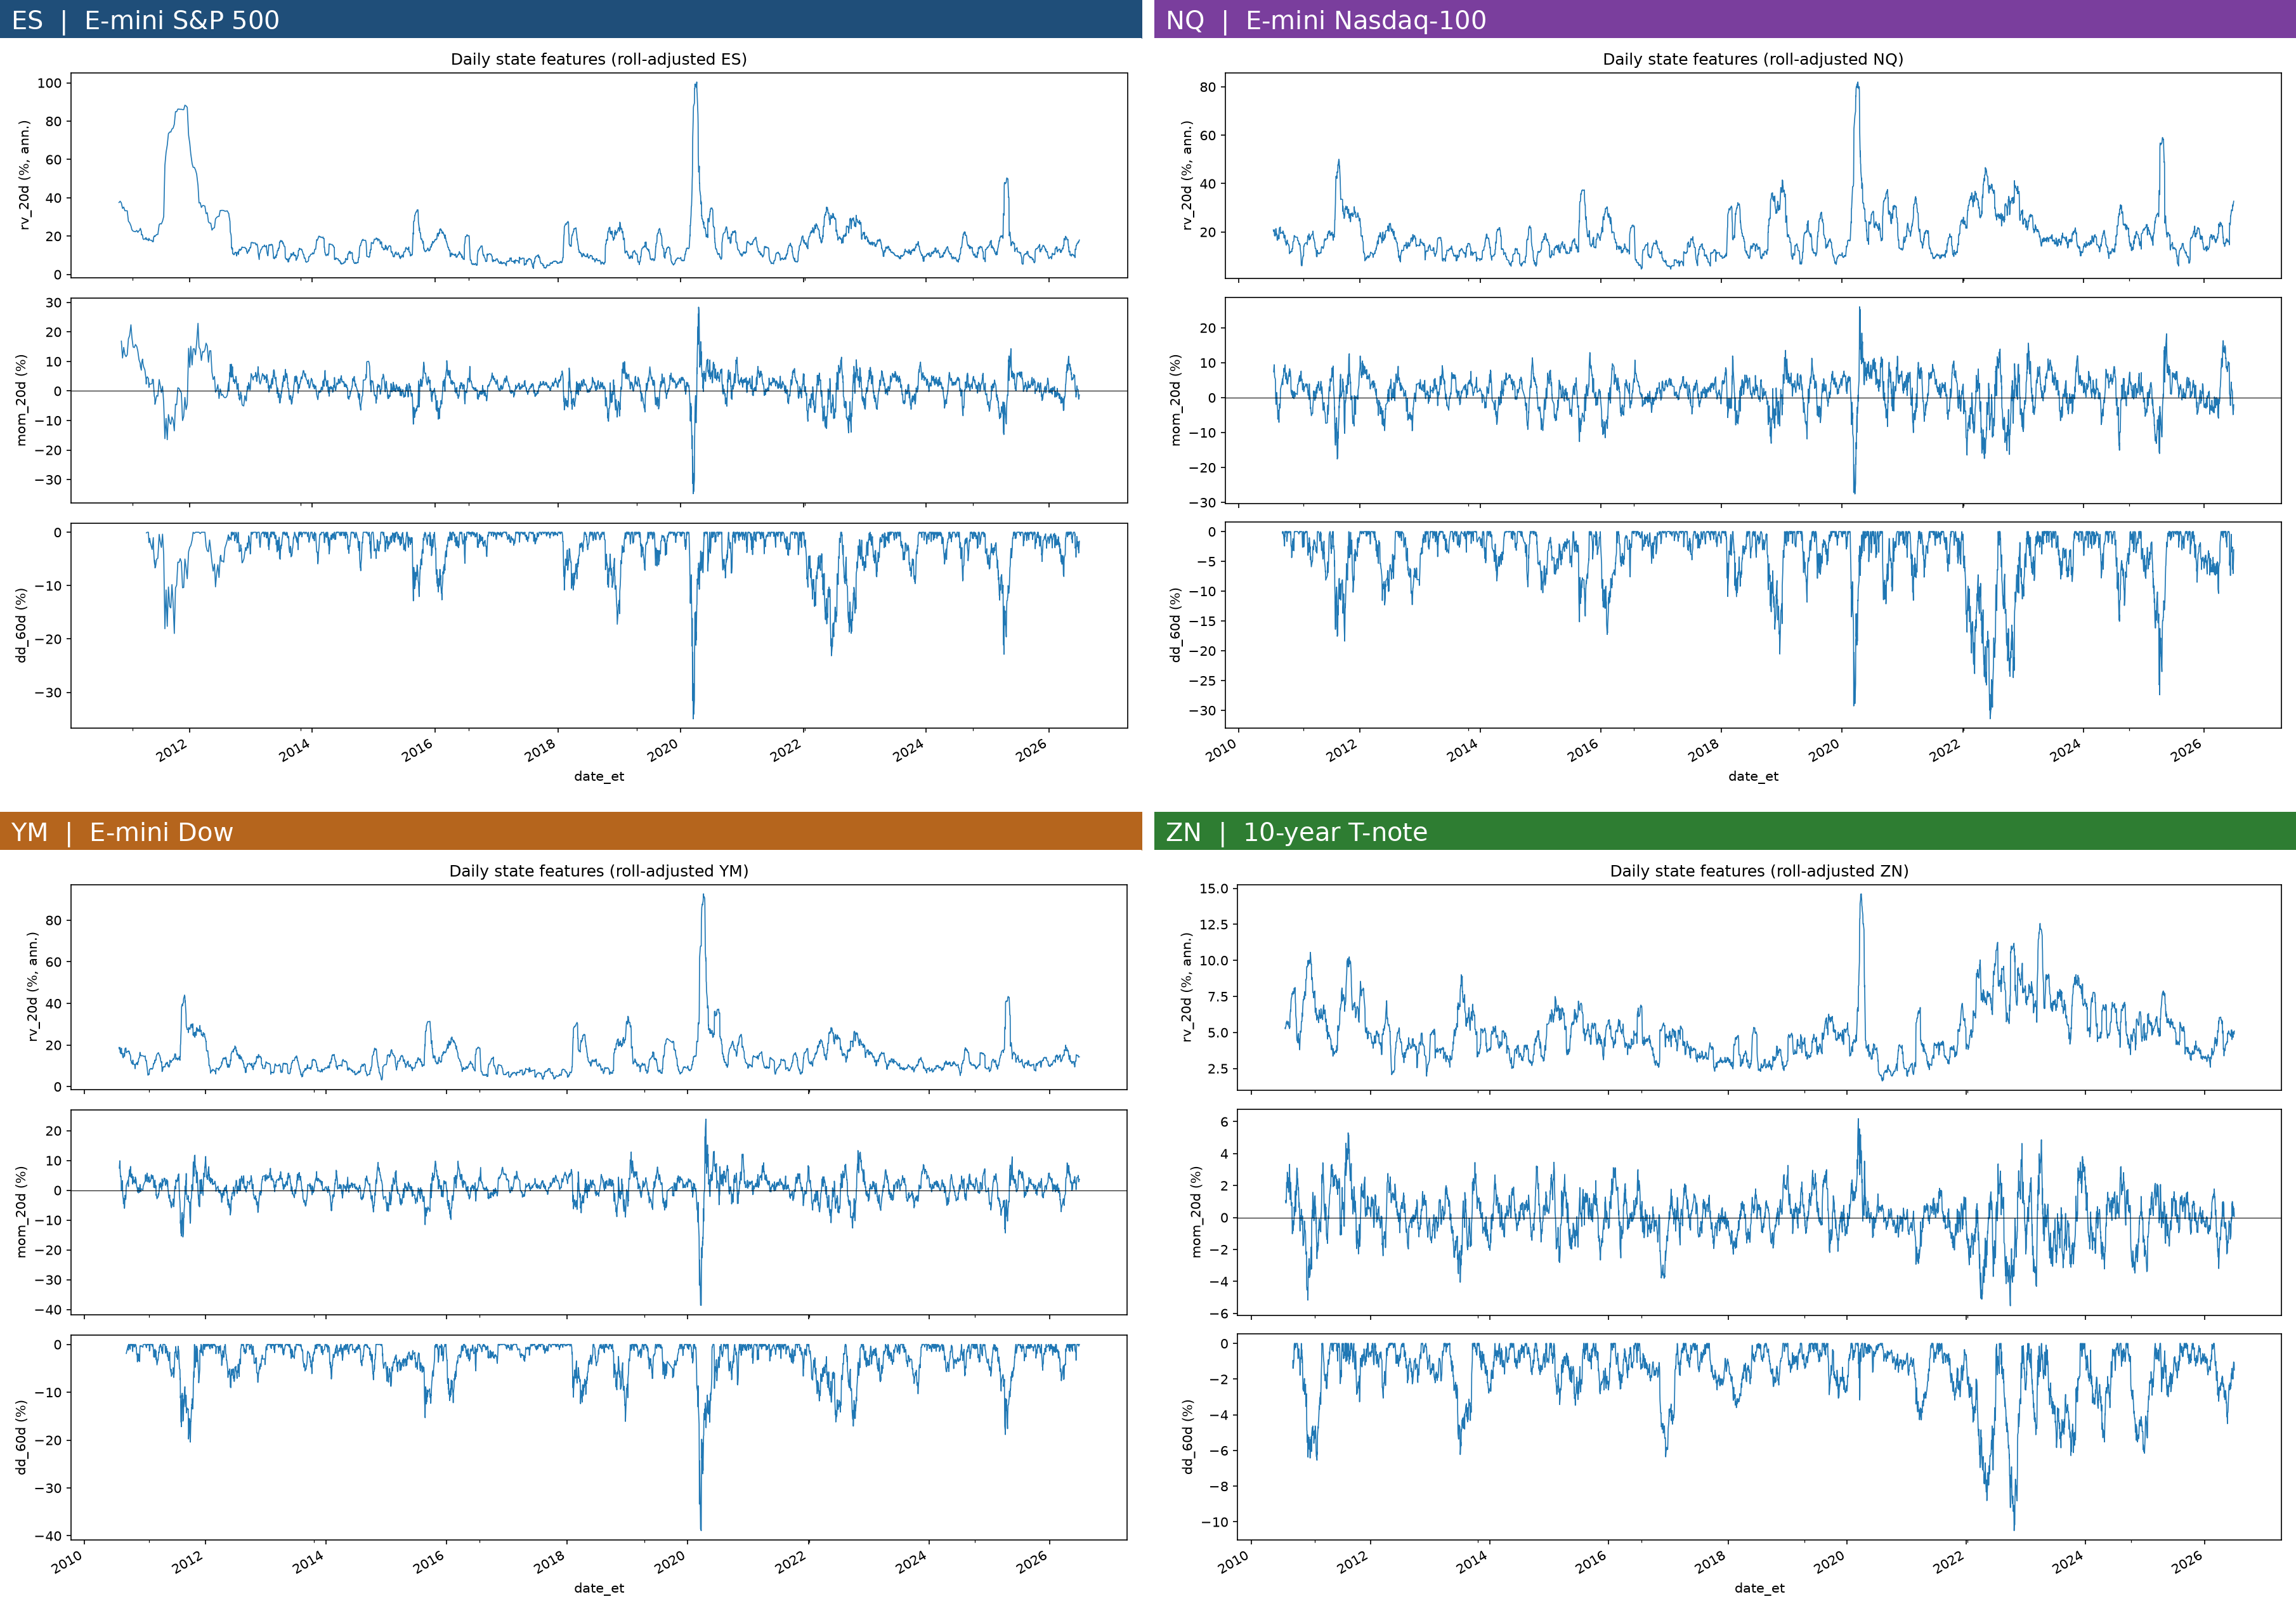
\includegraphics[width=\linewidth]{app_daily_state_4markets}
  \caption{Daily state features, 2010--2026: 20-day realized volatility (annualized \%), 20-day
  momentum (\%) and distance from the 60-day high (\%), computed on roll-adjusted daily closes. The
  2011 \ES\ volatility spike reflects incomplete sessions in the original vendor file.}
  \label{fig:app_daily_state}
\end{figure}

Figure~\ref{fig:app_buckets} splits the five-minute CPI beta by tercile of each pre-release state
in \ES\ and \YM. The beta rises from under 10 bps per standard deviation in the calmest third of
20-day volatility to 40--70 bps in the middle and top thirds in both markets, the clearest pattern among the
six states. Table~\ref{tab:app_state} lists the strongest of the 48 primary tests in
each market. Figure~\ref{fig:app_pvalues} shows that the analytic HC3 and permutation $p$-values
agree closely, so the inference does not depend on the normal approximation.

\begin{figure}[!htb]
  \centering
  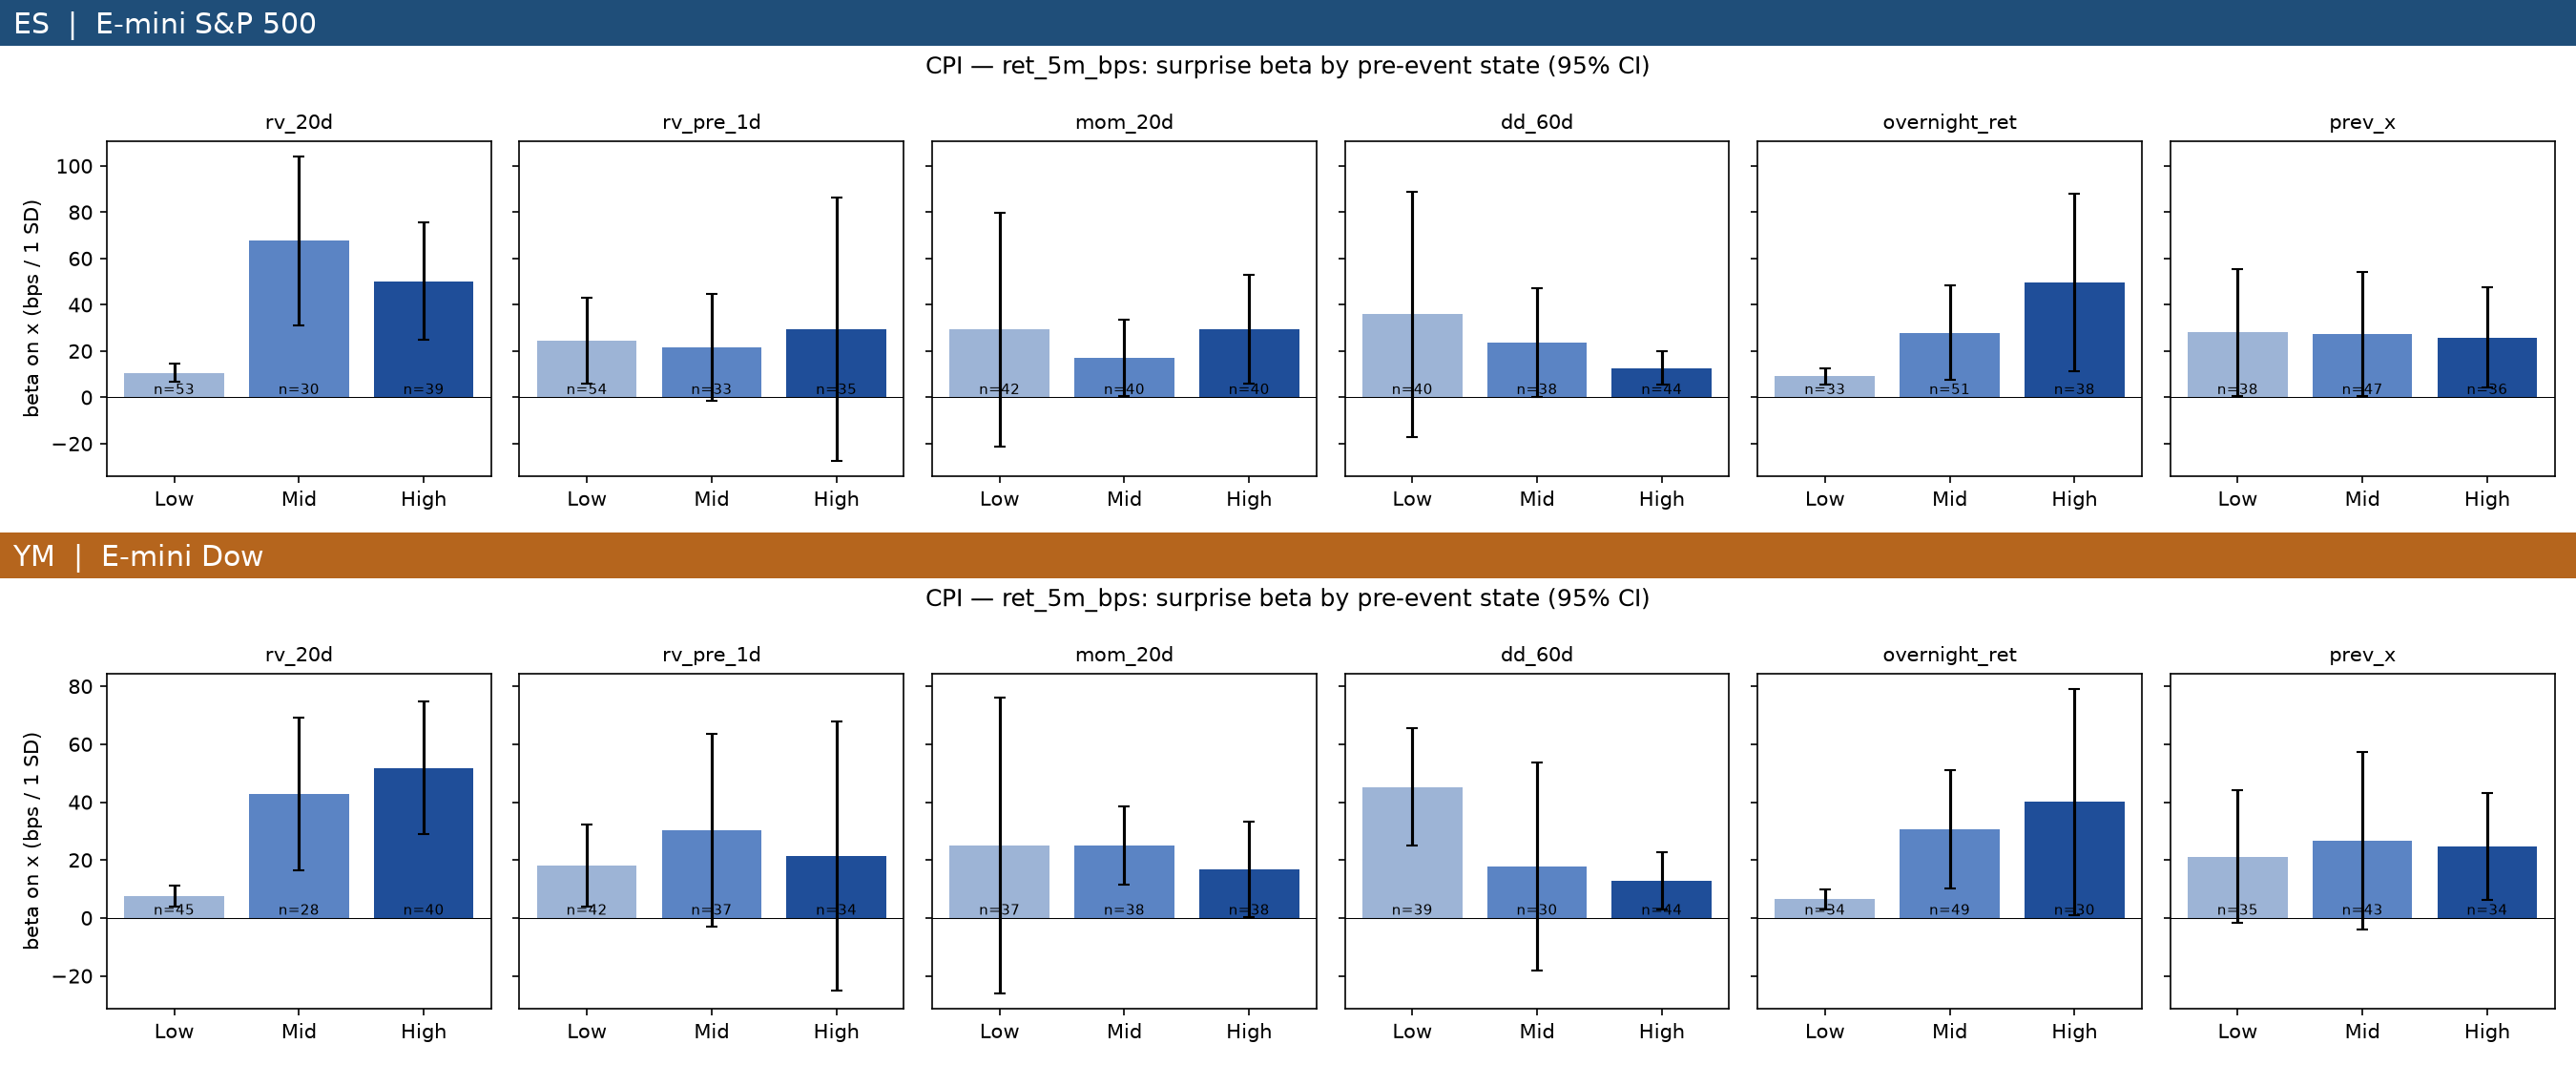
\includegraphics[width=\linewidth]{app_bucket_betas_ES_YM}
  \caption{Five-minute CPI surprise beta (bps per SD, 95\% intervals) by tercile of each
  pre-release state: 20-day realized volatility, previous-day volatility, 20-day momentum, 60-day
  drawdown, overnight return and previous surprise.}
  \label{fig:app_buckets}
\end{figure}

\begin{table}[!htb]
  \centering\small
  \caption{Strongest state interactions among the 48 primary tests, 2016--2026.}\label{tab:app_state}
  \begin{threeparttable}
  \begin{tabular}{lllcccc}
    \toprule
    Market & Interaction & Target & $d$ (bps) & $t$ (HC3) & $p$ (perm.) & $q$ (BH) \\
    \midrule
    \ES & CPI $\times$ 20-day vol & 5-min reaction & $+61.1$ & 3.81 & 0.000 & 0.010 \\
        & NFP $\times$ 20-day vol & 30-min drift & $-12.2$ & $-2.99$ & 0.016 & 0.082 \\
        & All $\times$ overnight return & 30-min drift & $+7.4$ & 2.65 & 0.021 & 0.134 \\
    \YM & CPI $\times$ 20-day vol & 5-min reaction & $+58.7$ & 3.74 & 0.004 & 0.014 \\
        & NFP $\times$ previous-day vol & 5-min reaction & $-21.0$ & $-3.07$ & 0.012 & 0.042 \\
        & NFP $\times$ 20-day vol & 5-min reaction & $-17.3$ & $-3.11$ & 0.014 & 0.042 \\
    \bottomrule
  \end{tabular}
  \begin{tablenotes}\footnotesize
    \item Notes: $d$ is the change in the surprise beta from the calmest to the most stressed state
    in equation~\eqref{eq:state}. $q$: Benjamini--Hochberg over the 48 primary tests per market. The
    NFP effects in \YM\ come entirely from 2016--2020.
  \end{tablenotes}
  \end{threeparttable}
\end{table}

\begin{figure}[!htb]
  \centering
  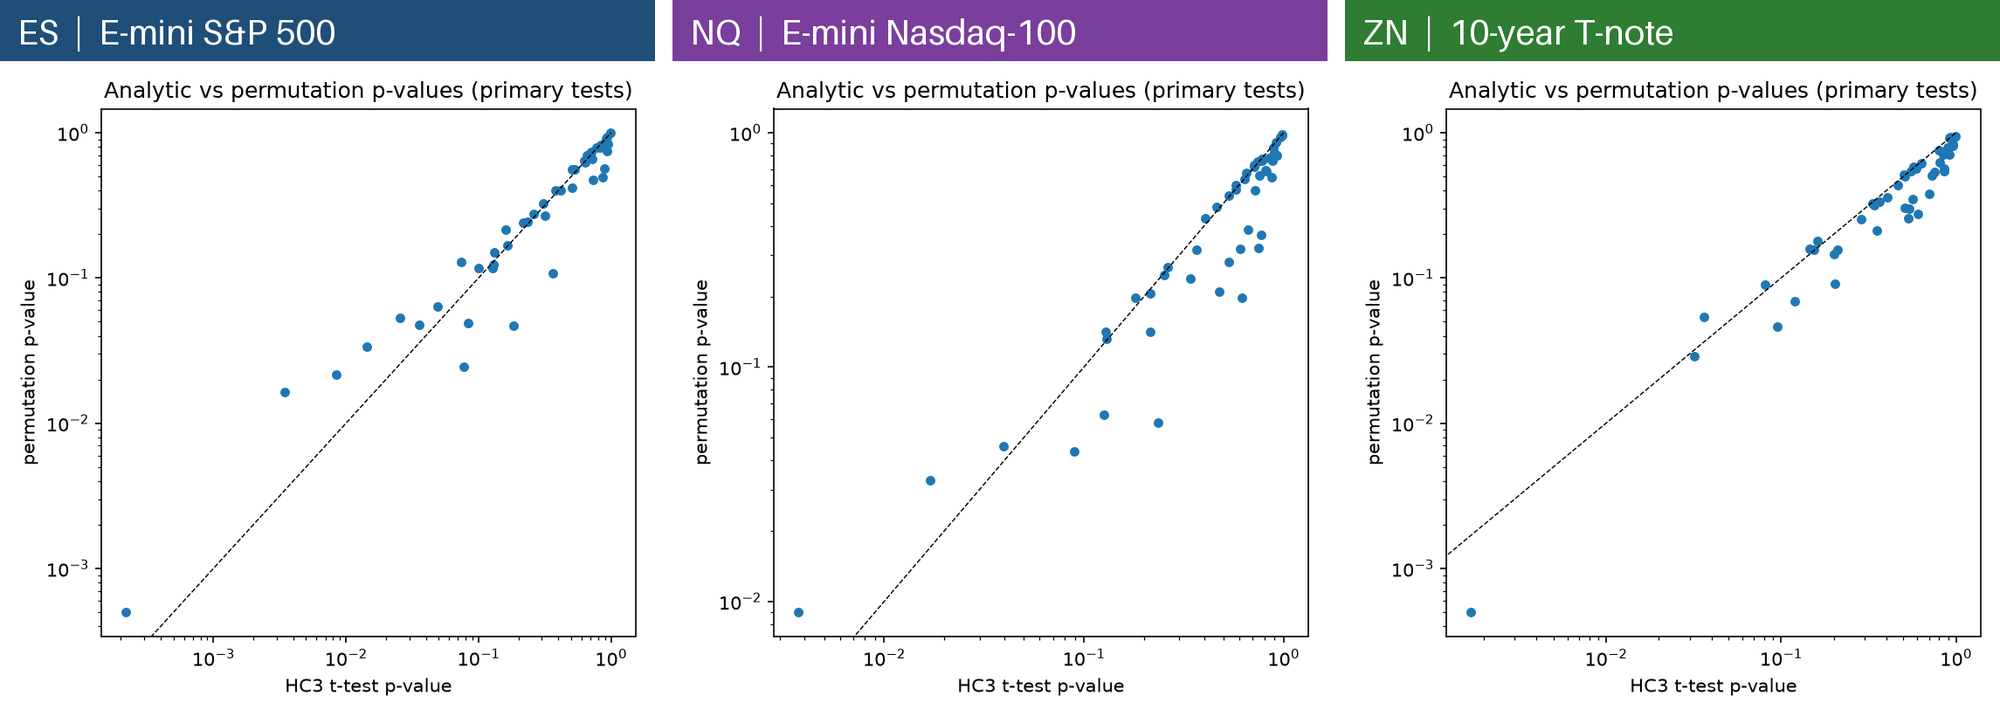
\includegraphics[width=\linewidth]{app_fig13_pvalue_comparison_3markets}
  \caption{Analytic (HC3) against permutation $p$-values for the primary state tests, \ES, \NQ\ and \ZN.}
  \label{fig:app_pvalues}
\end{figure}

\paragraph{Interaction regressions (notebook 03, section 9).} Rather than splitting the releases
into terciles, the interaction regression uses the full sample at once. For release $i$,
\begin{equation}\label{eq:app_inter}
  r_i = a + b\,x_i + c\,s_i + d\,(x_i\times s_i) + \varepsilon_i,\qquad s_i=\text{pct}_i-0.5,
\end{equation}
where $x_i$ is the signed surprise and $\text{pct}_i$ the percentile of the state against its
trailing one-year distribution. Centering the state makes $b$ the surprise beta at the median
state; $c$ asks whether the state predicts the return on its own; and $d$, the key coefficient, is
the change in the surprise beta from the lowest to the highest state percentile. Because $x$ is
signed so that $b>0$, a positive $d$ means a stronger reaction in the high state. The pooled model
(\texttt{ALL}) gives each family its own intercept and slope but a common $c$ and $d$. Each market
has 360 regressions: ten states (six primary, four exploratory), four families (CPI, NFP, PCE and
pooled) and nine targets (the reaction from the pre-release price at 1--60 minutes and the drift
from one minute after the release at 5--60 minutes). Standard errors are HC3. The 48 primary tests
(six states, four families, two targets: the five-minute reaction and the 30-minute drift) also get
a 2,000-draw permutation test and the Benjamini--Hochberg correction. A credible state effect looks
like a row of same-colored cells across horizons; a single bold cell among about 90 is what chance
produces, since at 5\% significance four to five false positives are expected per heat map.

The CPI heat maps are in Figure~\ref{fig:state} of the main text. Figures~\ref{fig:app_inter_nfp}--\ref{fig:app_inter_all}
show the other families. For payrolls (Figure~\ref{fig:app_inter_nfp}), the volatility rows are
negative: strong payrolls help equities less when volatility is high. The pattern is strongest in
\YM, where both 20-day and previous-day volatility have $t$-statistics of $-3.1$ to $-4.5$ on the
5- to 60-minute reactions, and present in \ES\ on the drifts; but in \YM\ it comes entirely from 2016--2020,
so it is not used for trading. PCE (Figure~\ref{fig:app_inter_pce}) shows only scattered cells with
no consistent row, as expected for a release whose surprise explains little of the move. In the
pooled model (Figure~\ref{fig:app_inter_all}), the overnight return and 5-day momentum rows are
positive on the 15--60-minute drifts in \ES\ and \YM\ ($t$ of 2.1--2.9): the drift follows the surprise
more strongly after a market has already been rising. Only the \ES\ overnight-return effect on the
30-minute drift is a primary test, and it does not survive the correction ($q=0.13$). In \ZN, the
previous-day volatility row is negative on every drift ($t$ of $-2.1$ to $-3.2$): after volatile
days, the little drift \ZN\ has is even smaller.

\begin{figure}[!htb]
  \centering
  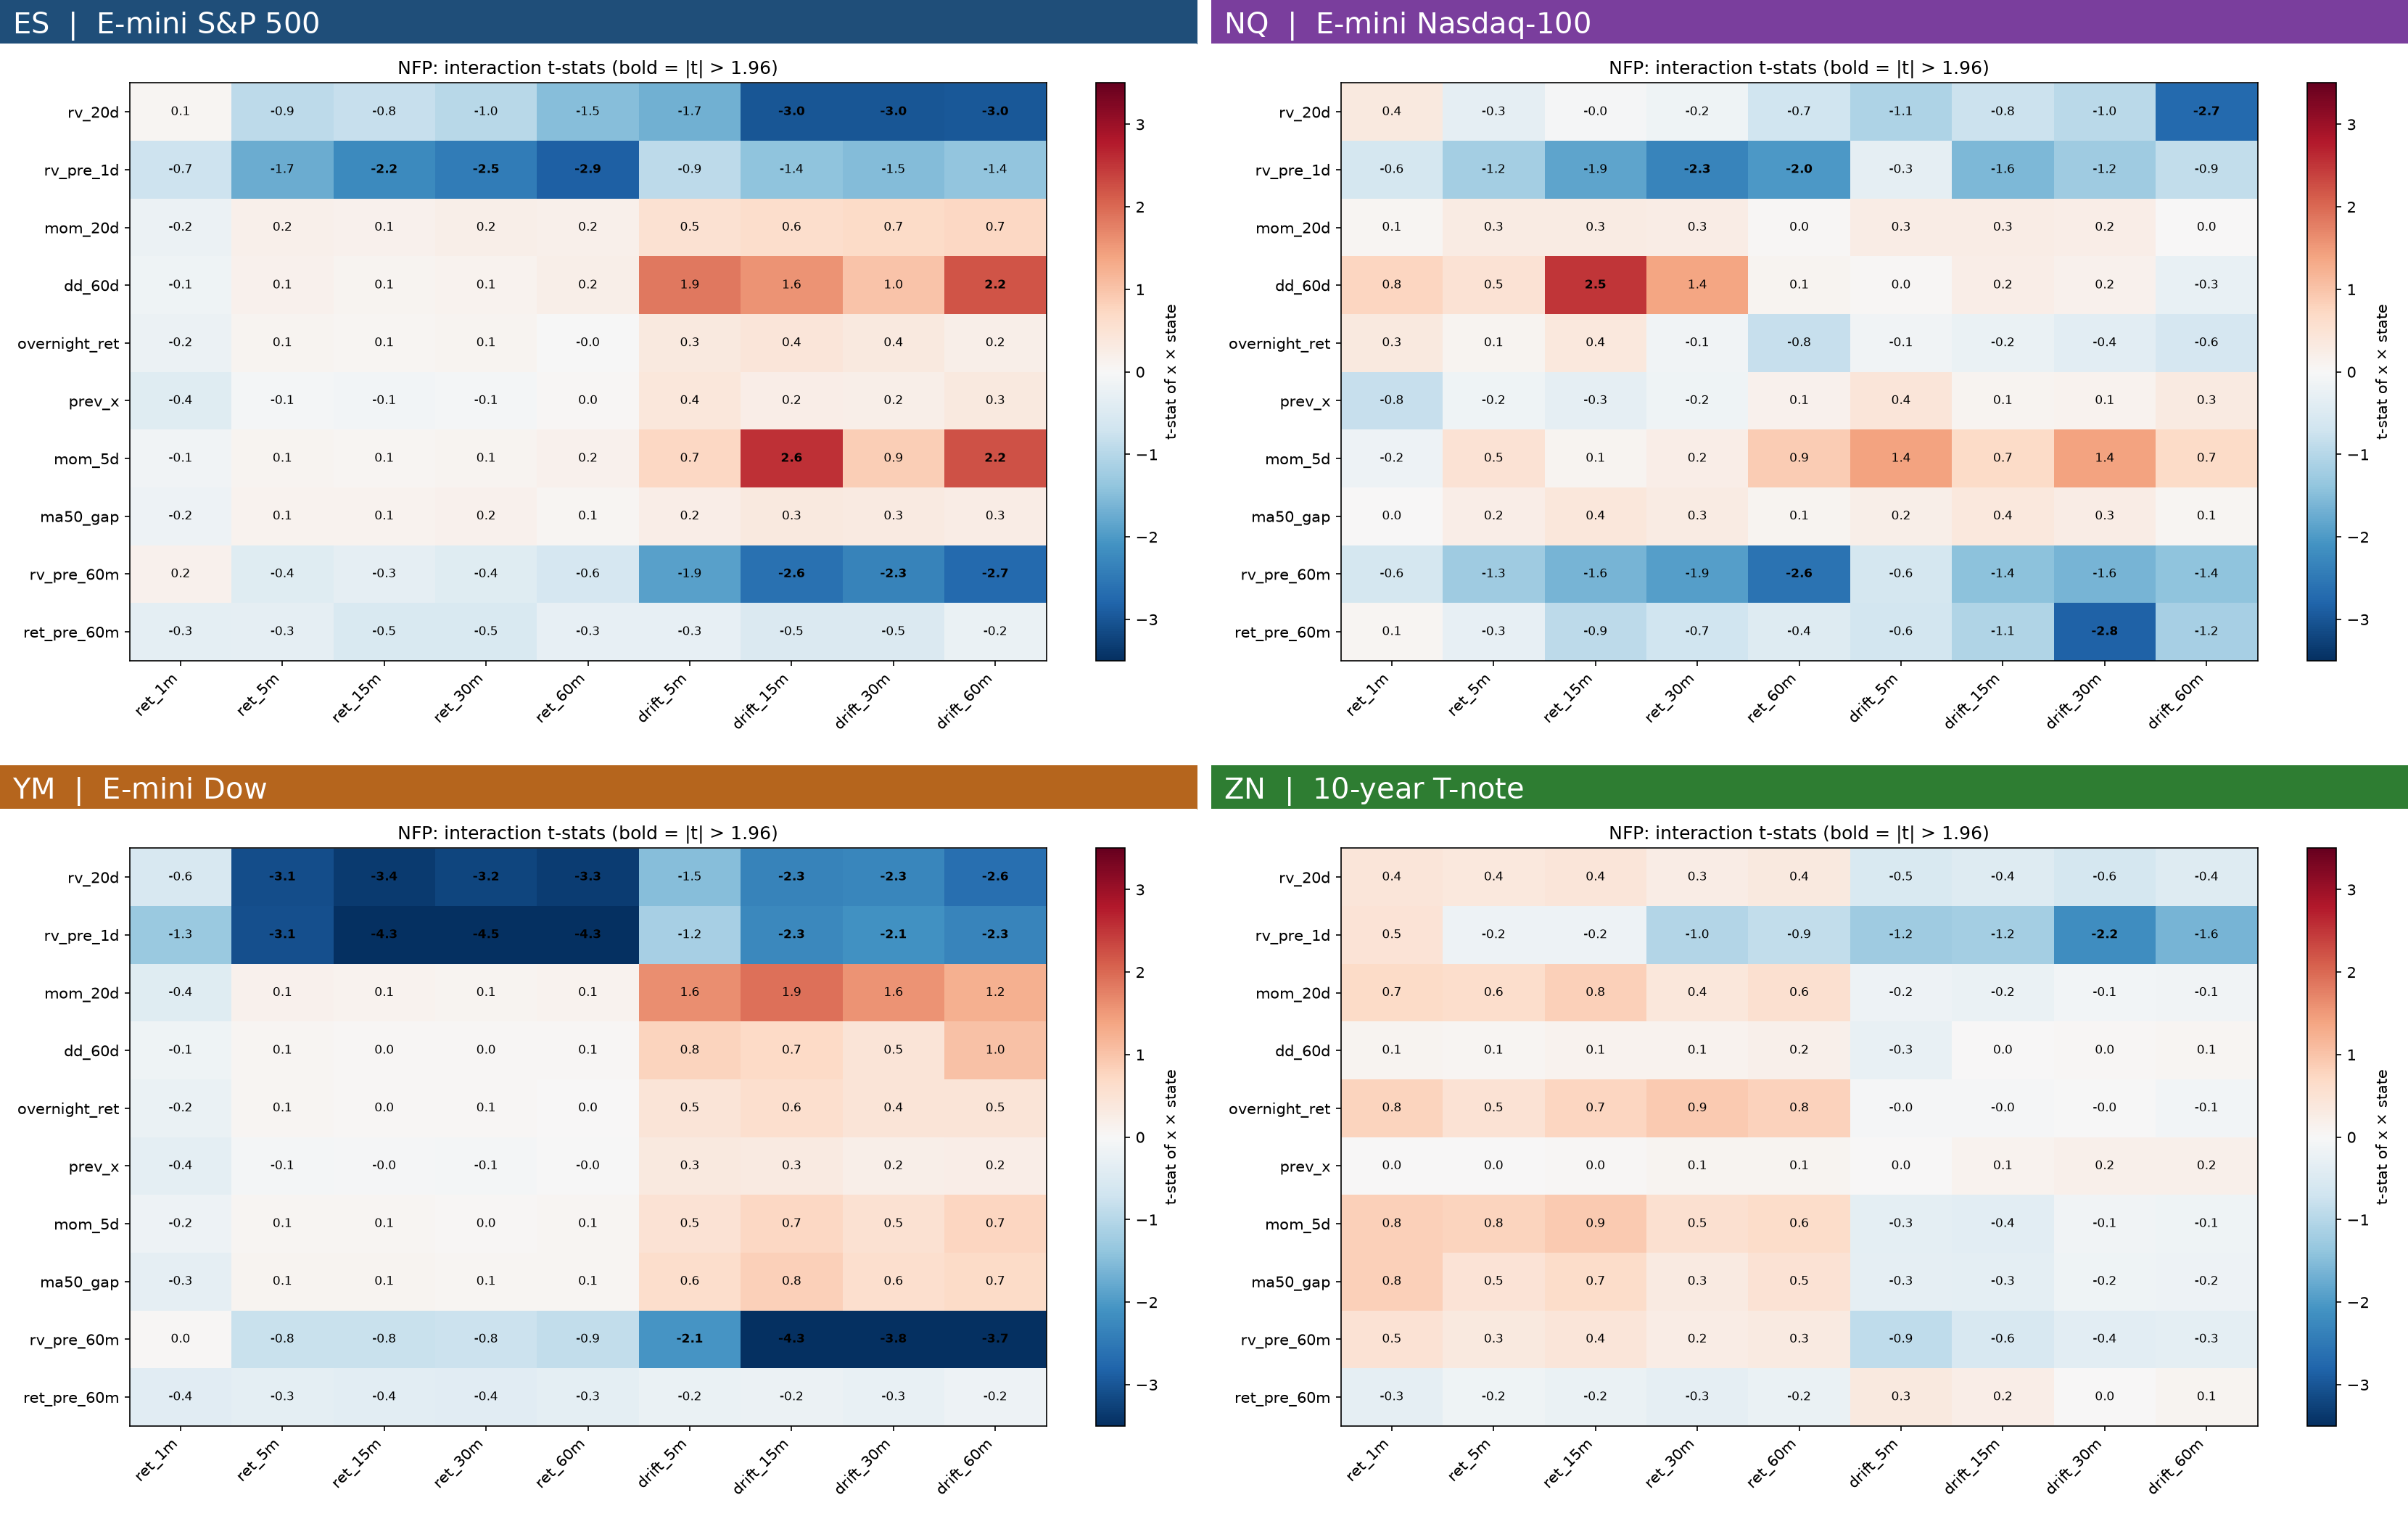
\includegraphics[width=\linewidth]{app_interaction_NFP_4markets}
  \caption{Payrolls (NFP): $t$-statistics of the surprise $\times$ state interaction $d$ in
  equation~\eqref{eq:app_inter}, by state (rows) and target (columns). Bold: $|t|>1.96$.}
  \label{fig:app_inter_nfp}
\end{figure}

\begin{figure}[!htb]
  \centering
  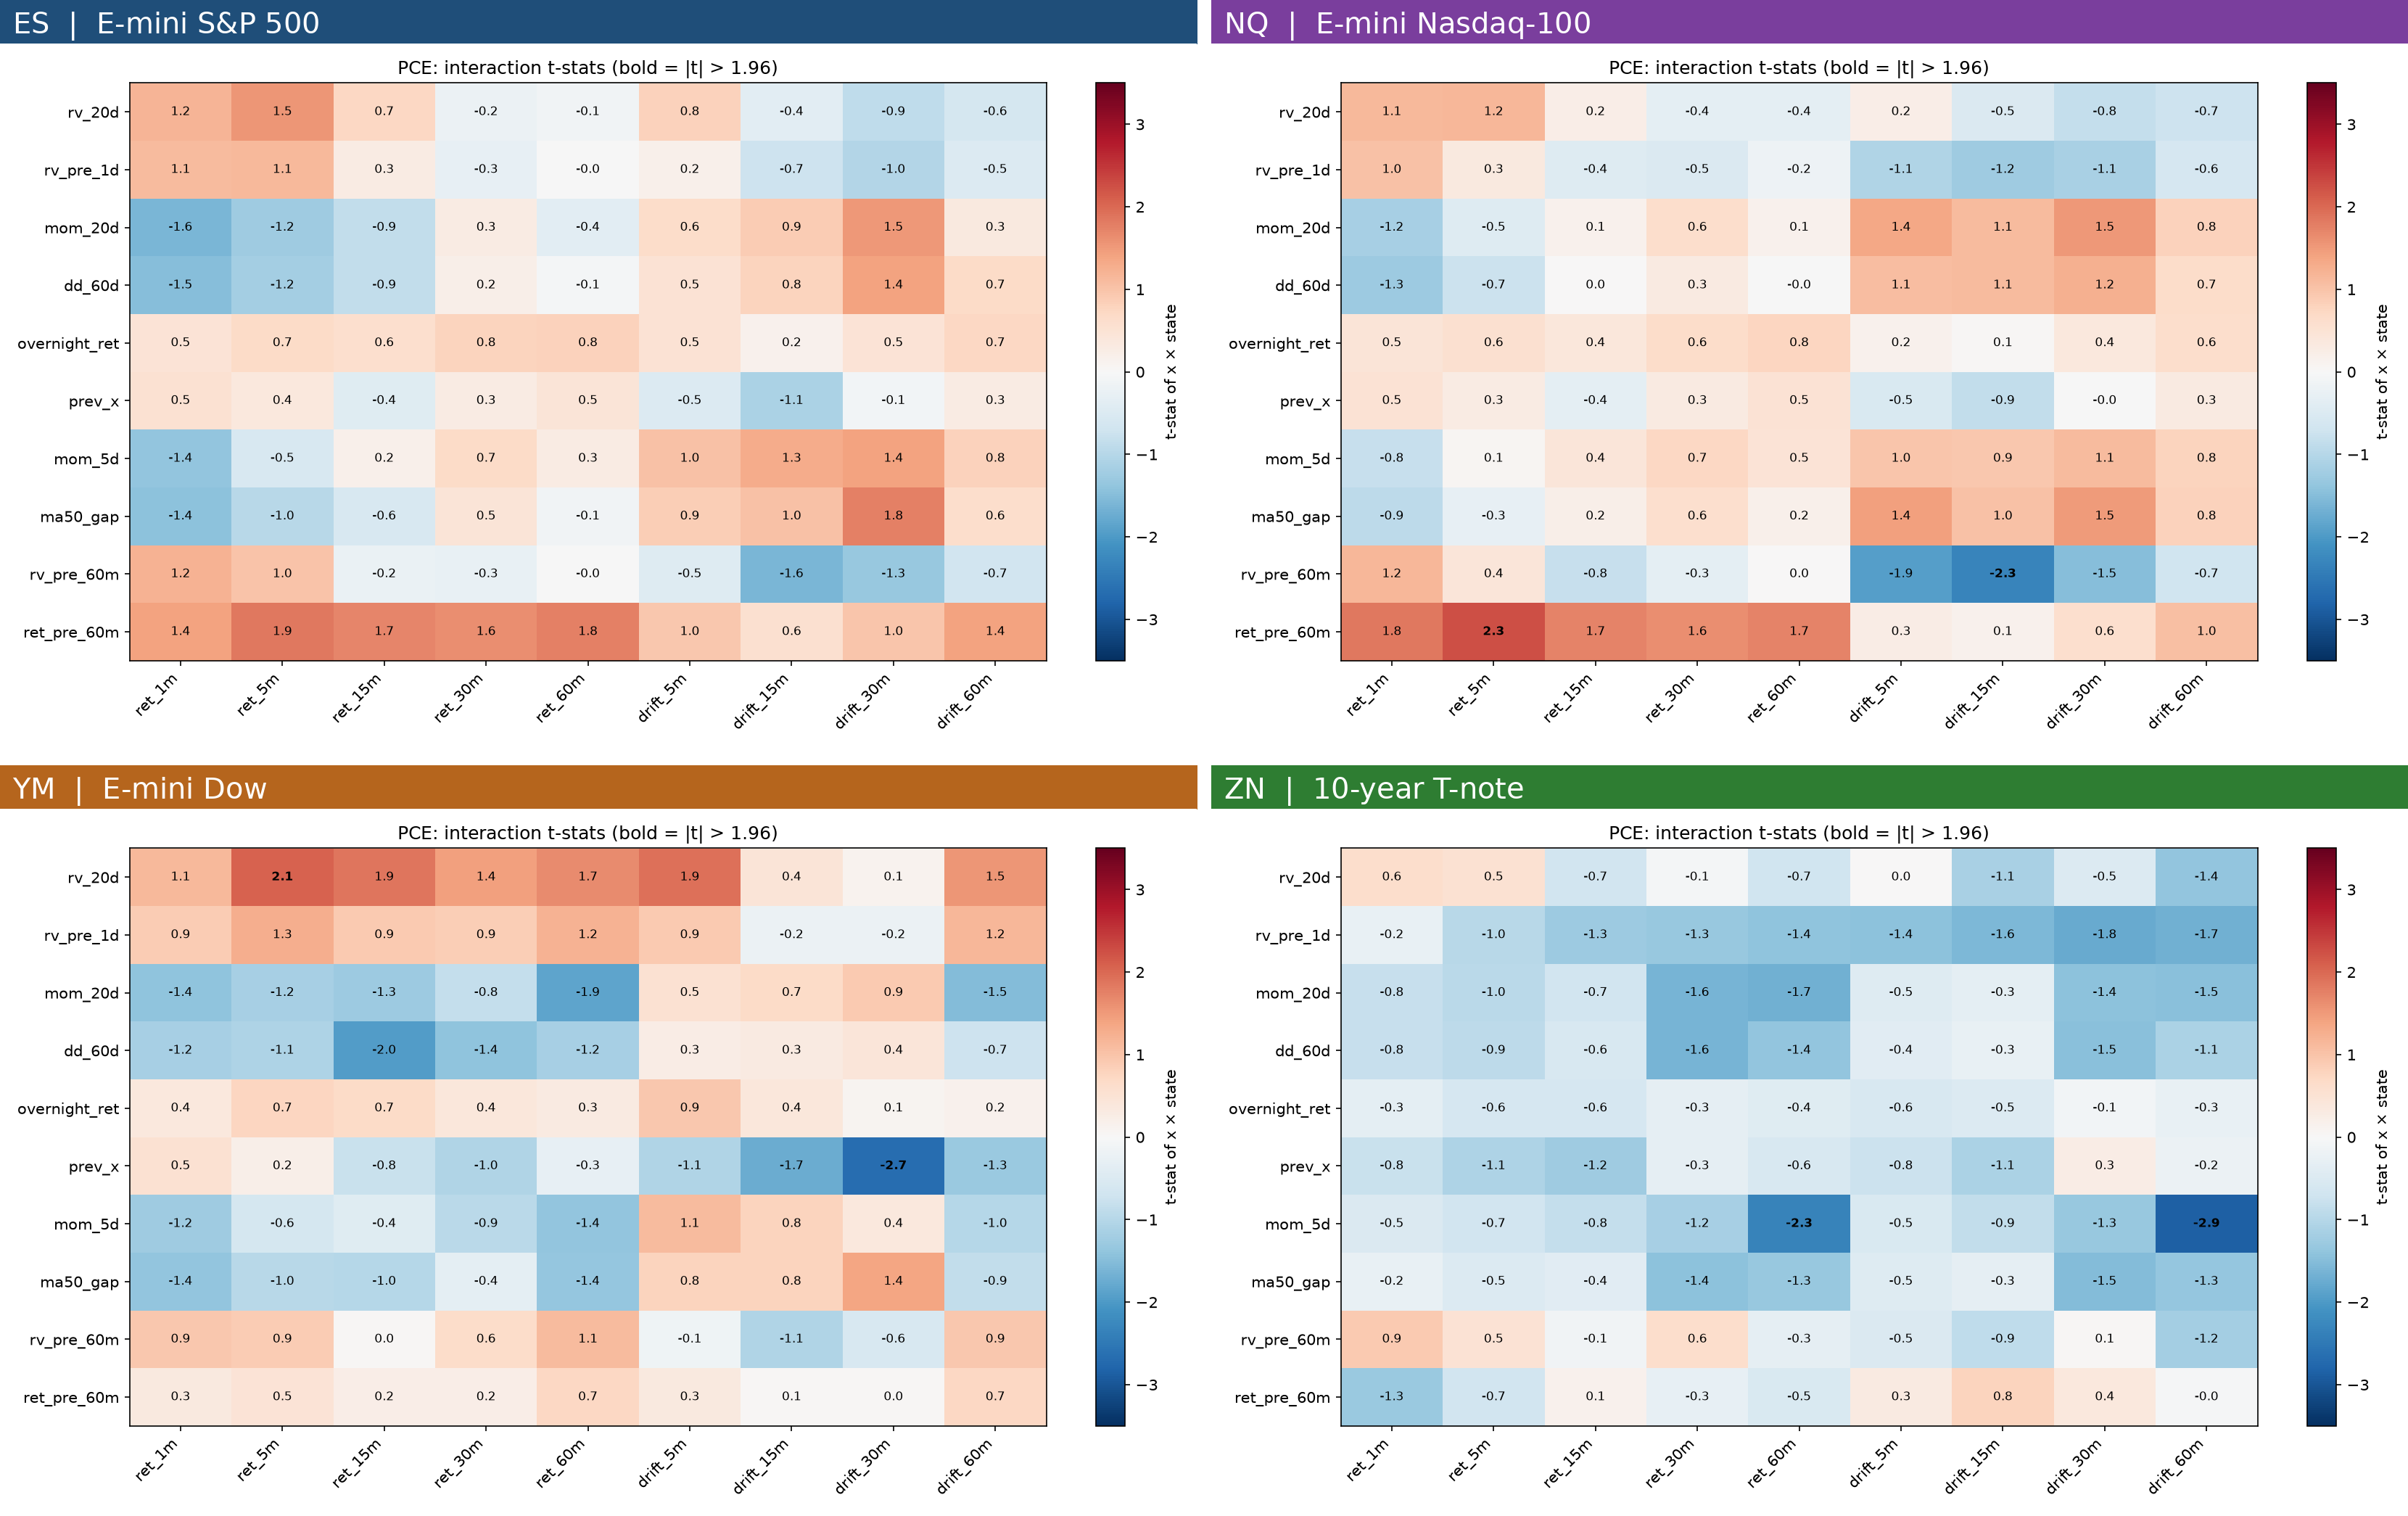
\includegraphics[width=\linewidth]{app_interaction_PCE_4markets}
  \caption{PCE: $t$-statistics of the surprise $\times$ state interaction $d$, by state and target.}
  \label{fig:app_inter_pce}
\end{figure}

\begin{figure}[!htb]
  \centering
  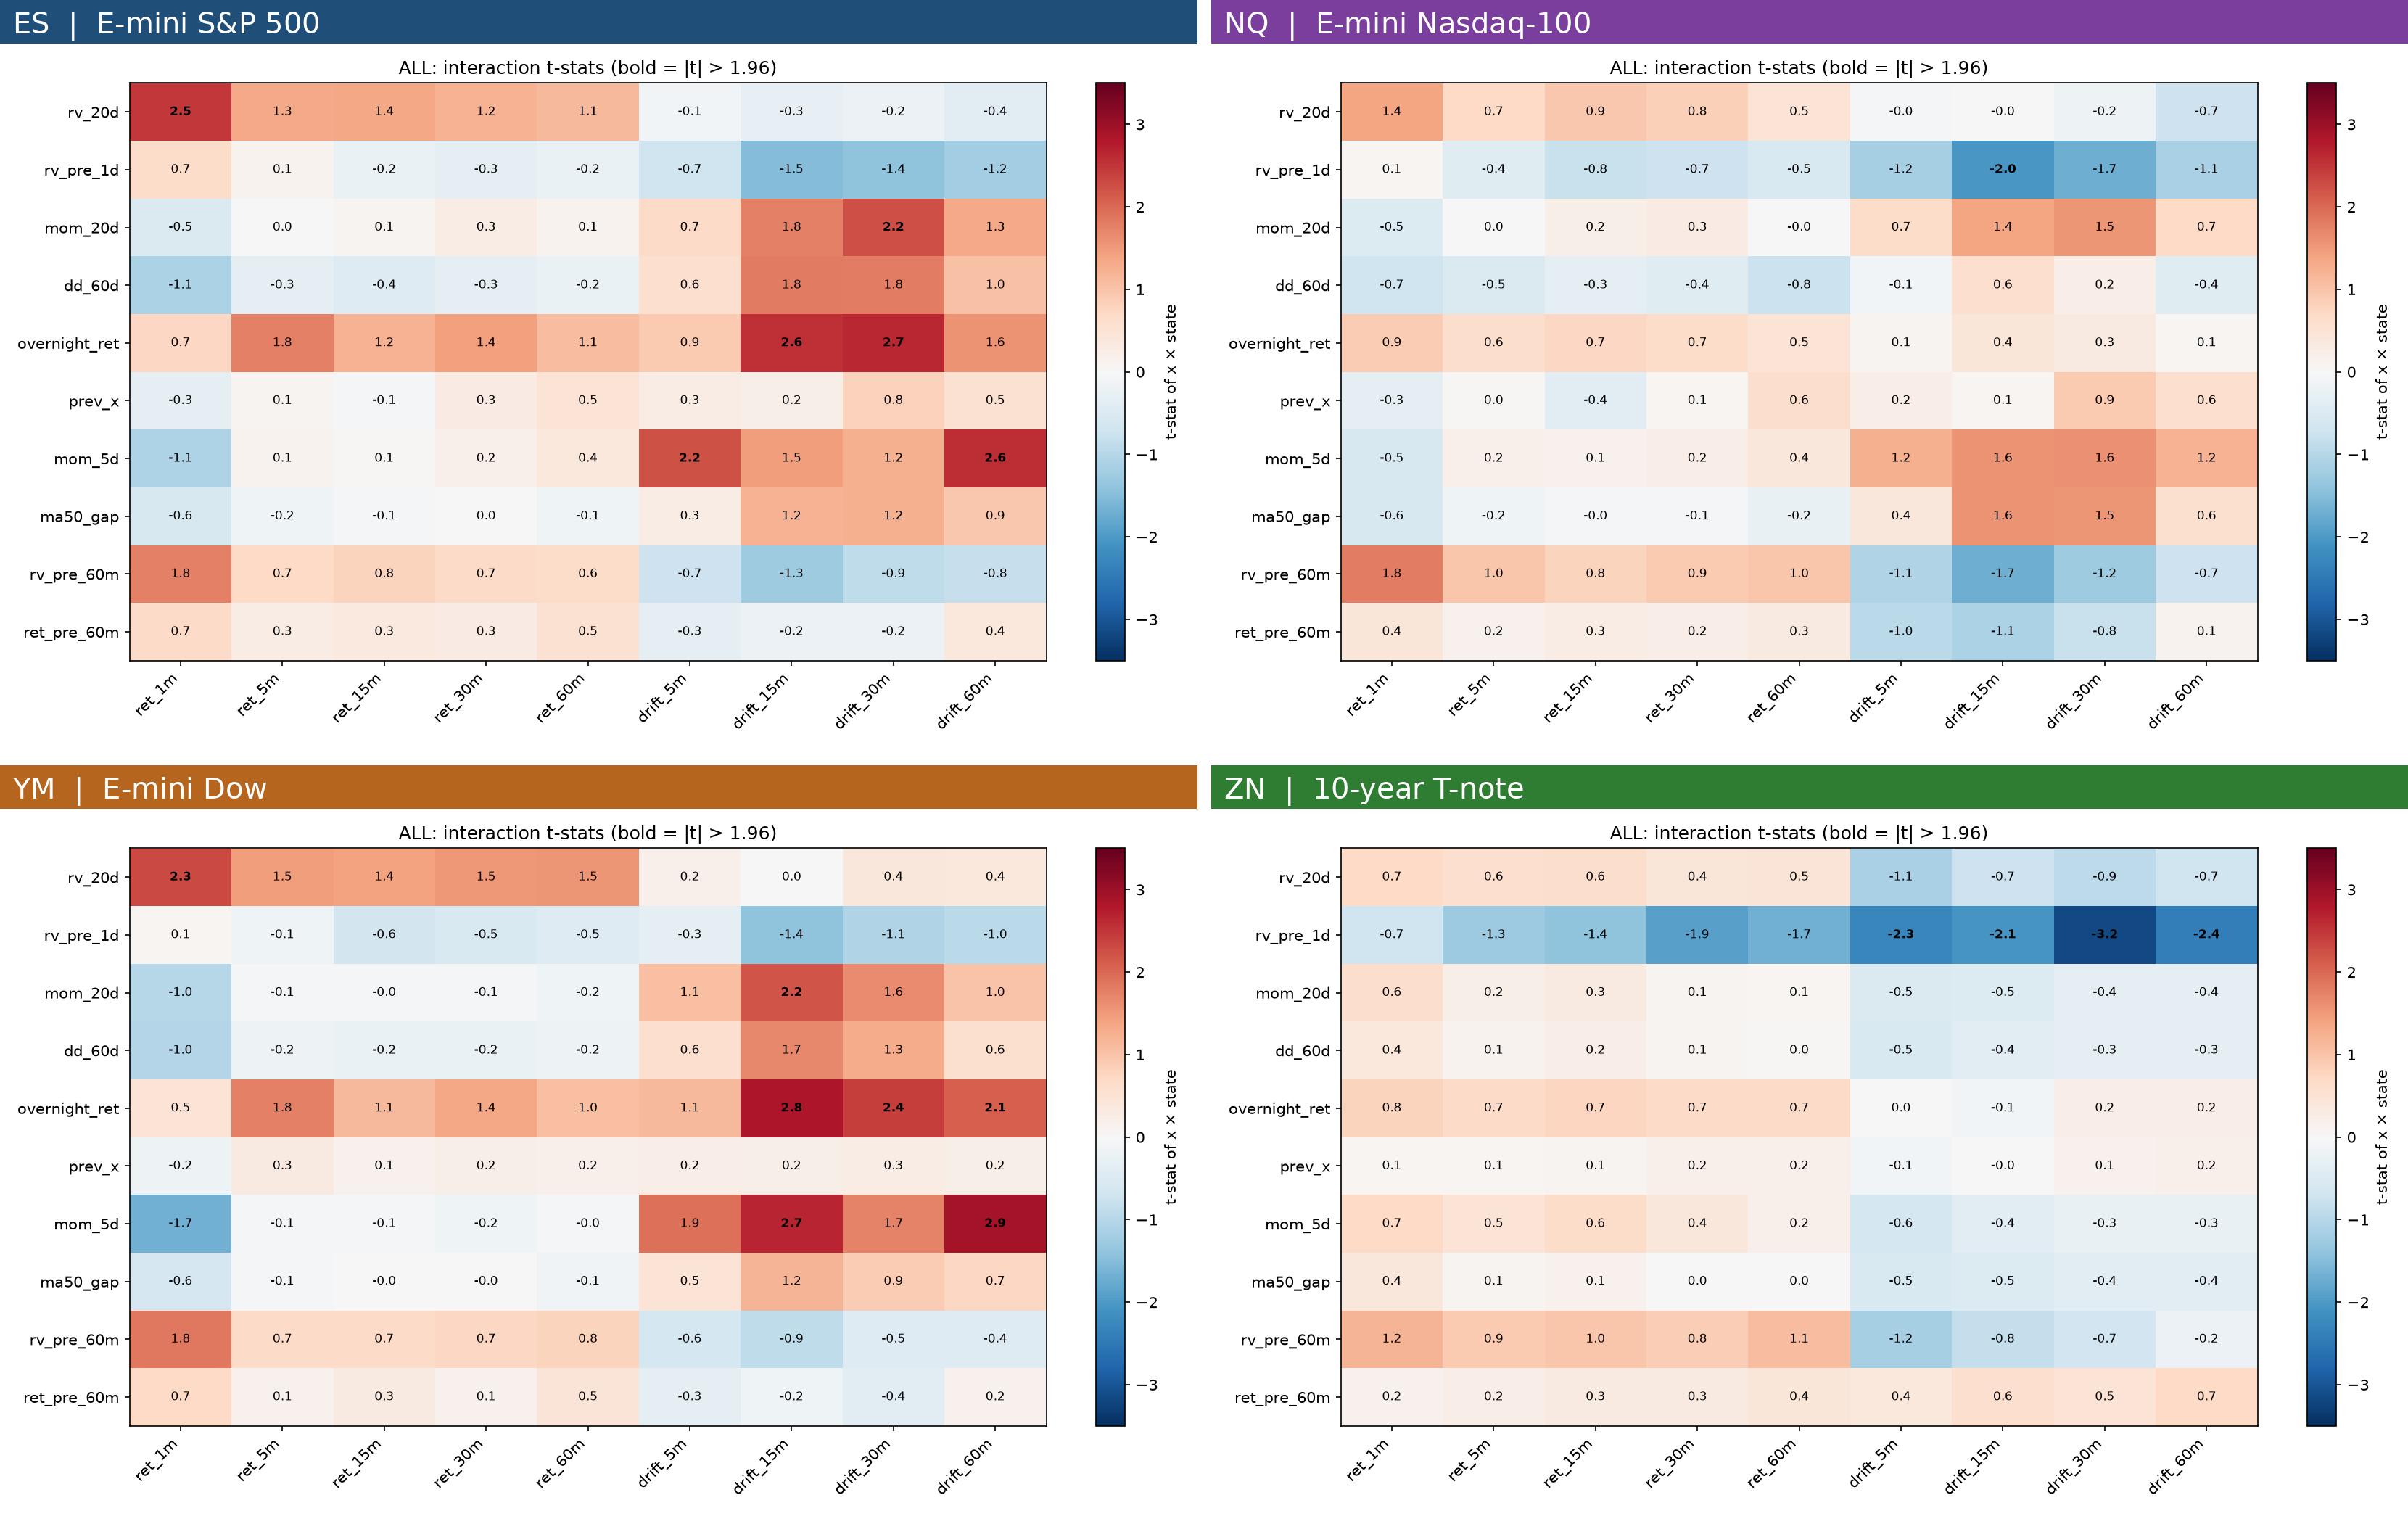
\includegraphics[width=\linewidth]{app_interaction_ALL_4markets}
  \caption{All three families pooled (family-specific intercepts and slopes, common $c$ and $d$):
  $t$-statistics of the surprise $\times$ state interaction, by state and target.}
  \label{fig:app_inter_all}
\end{figure}

\FloatBarrier
\subsection{Walk-forward CPI strategy (notebook 04)}

Figure~\ref{fig:app_latency} shows how the CPI strategy's Sharpe ratio changes with the entry
delay and the exit time. In both \ES\ and \YM\ the 30-minute exit is the best column at every
delay, and short holds lose most of their value when the entry is delayed. Figure~\ref{fig:app_paths}
shows the walk-forward estimates behind the state model: the CPI drift slope in \ES\
fell to about 1 bp per standard deviation in 2021 and rose to 6--8 bps from 2023, and the
$t$-statistic of the volatility interaction stays below about 2 until 2022 in \ES\ and \NQ\ and
never reaches it in \ZN.
Figures~\ref{fig:app_peer}--\ref{fig:app_peer_all} show the walk-forward strategies in the peer
chart format (notebook 04, section 16.5): the strategy before and after costs against being
always long, one contract, in exactly the same 30-minute windows. In the three equity indices the
strategies and the always-long line diverge from 2022: trading the CPI surprise gains 6.6\% in
\ES, 7.5\% in \NQ\ and 5.0\% in \YM\ while always long in the same windows loses 5--6\%, so the
profit comes from the direction of the surprise, not from being in the market at release times.
The naive sign rule and the model on CPI, PCE and payrolls show the same pattern. In \ZN\ the
surprise model trades only a handful of releases, because its predicted drift rarely exceeds the
cost of one \ZN\ tick, and the naive rule loses after costs.

\begin{figure}[!htb]
  \centering
  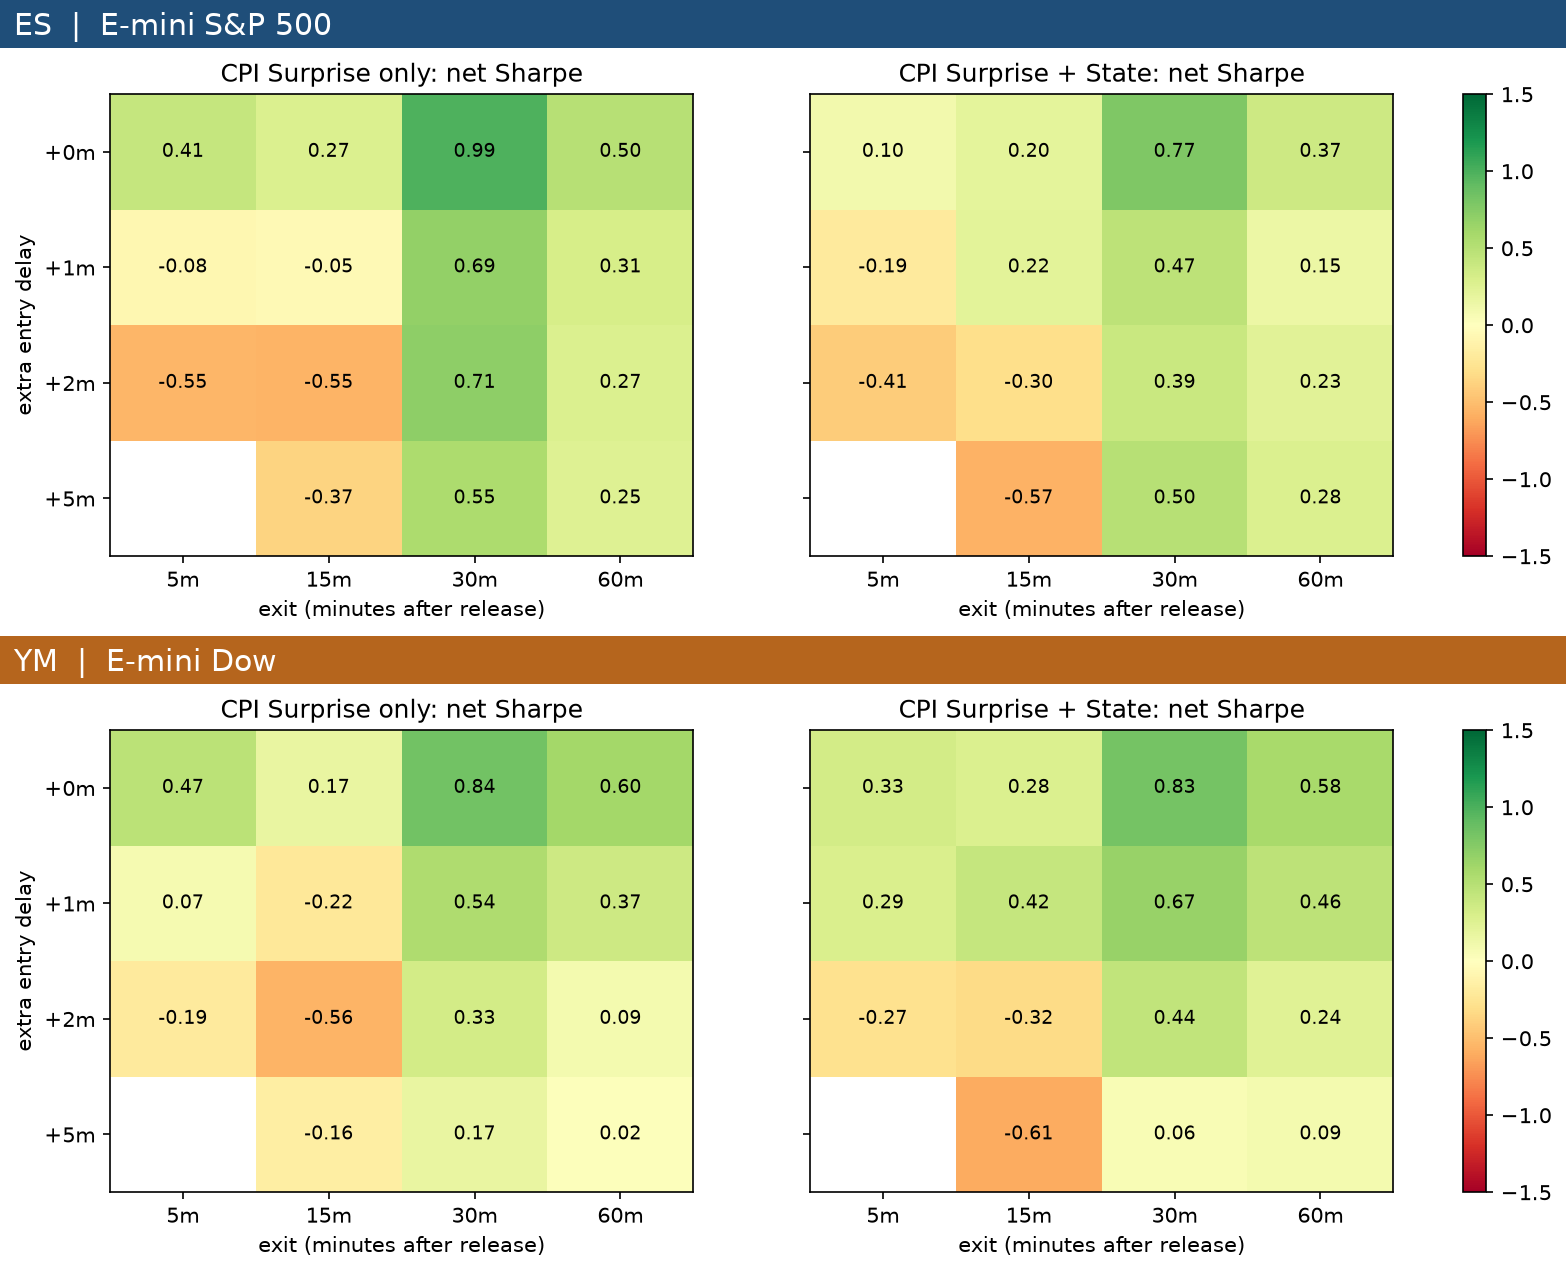
\includegraphics[width=0.85\linewidth]{app_latency_grid_ES_YM}
  \caption{Net Sharpe ratio of the CPI strategies by extra entry delay (rows) and exit time
  (columns), 2019--2026. Left: surprise only; right: surprise and state.}
  \label{fig:app_latency}
\end{figure}

\begin{figure}[!htb]
  \centering
  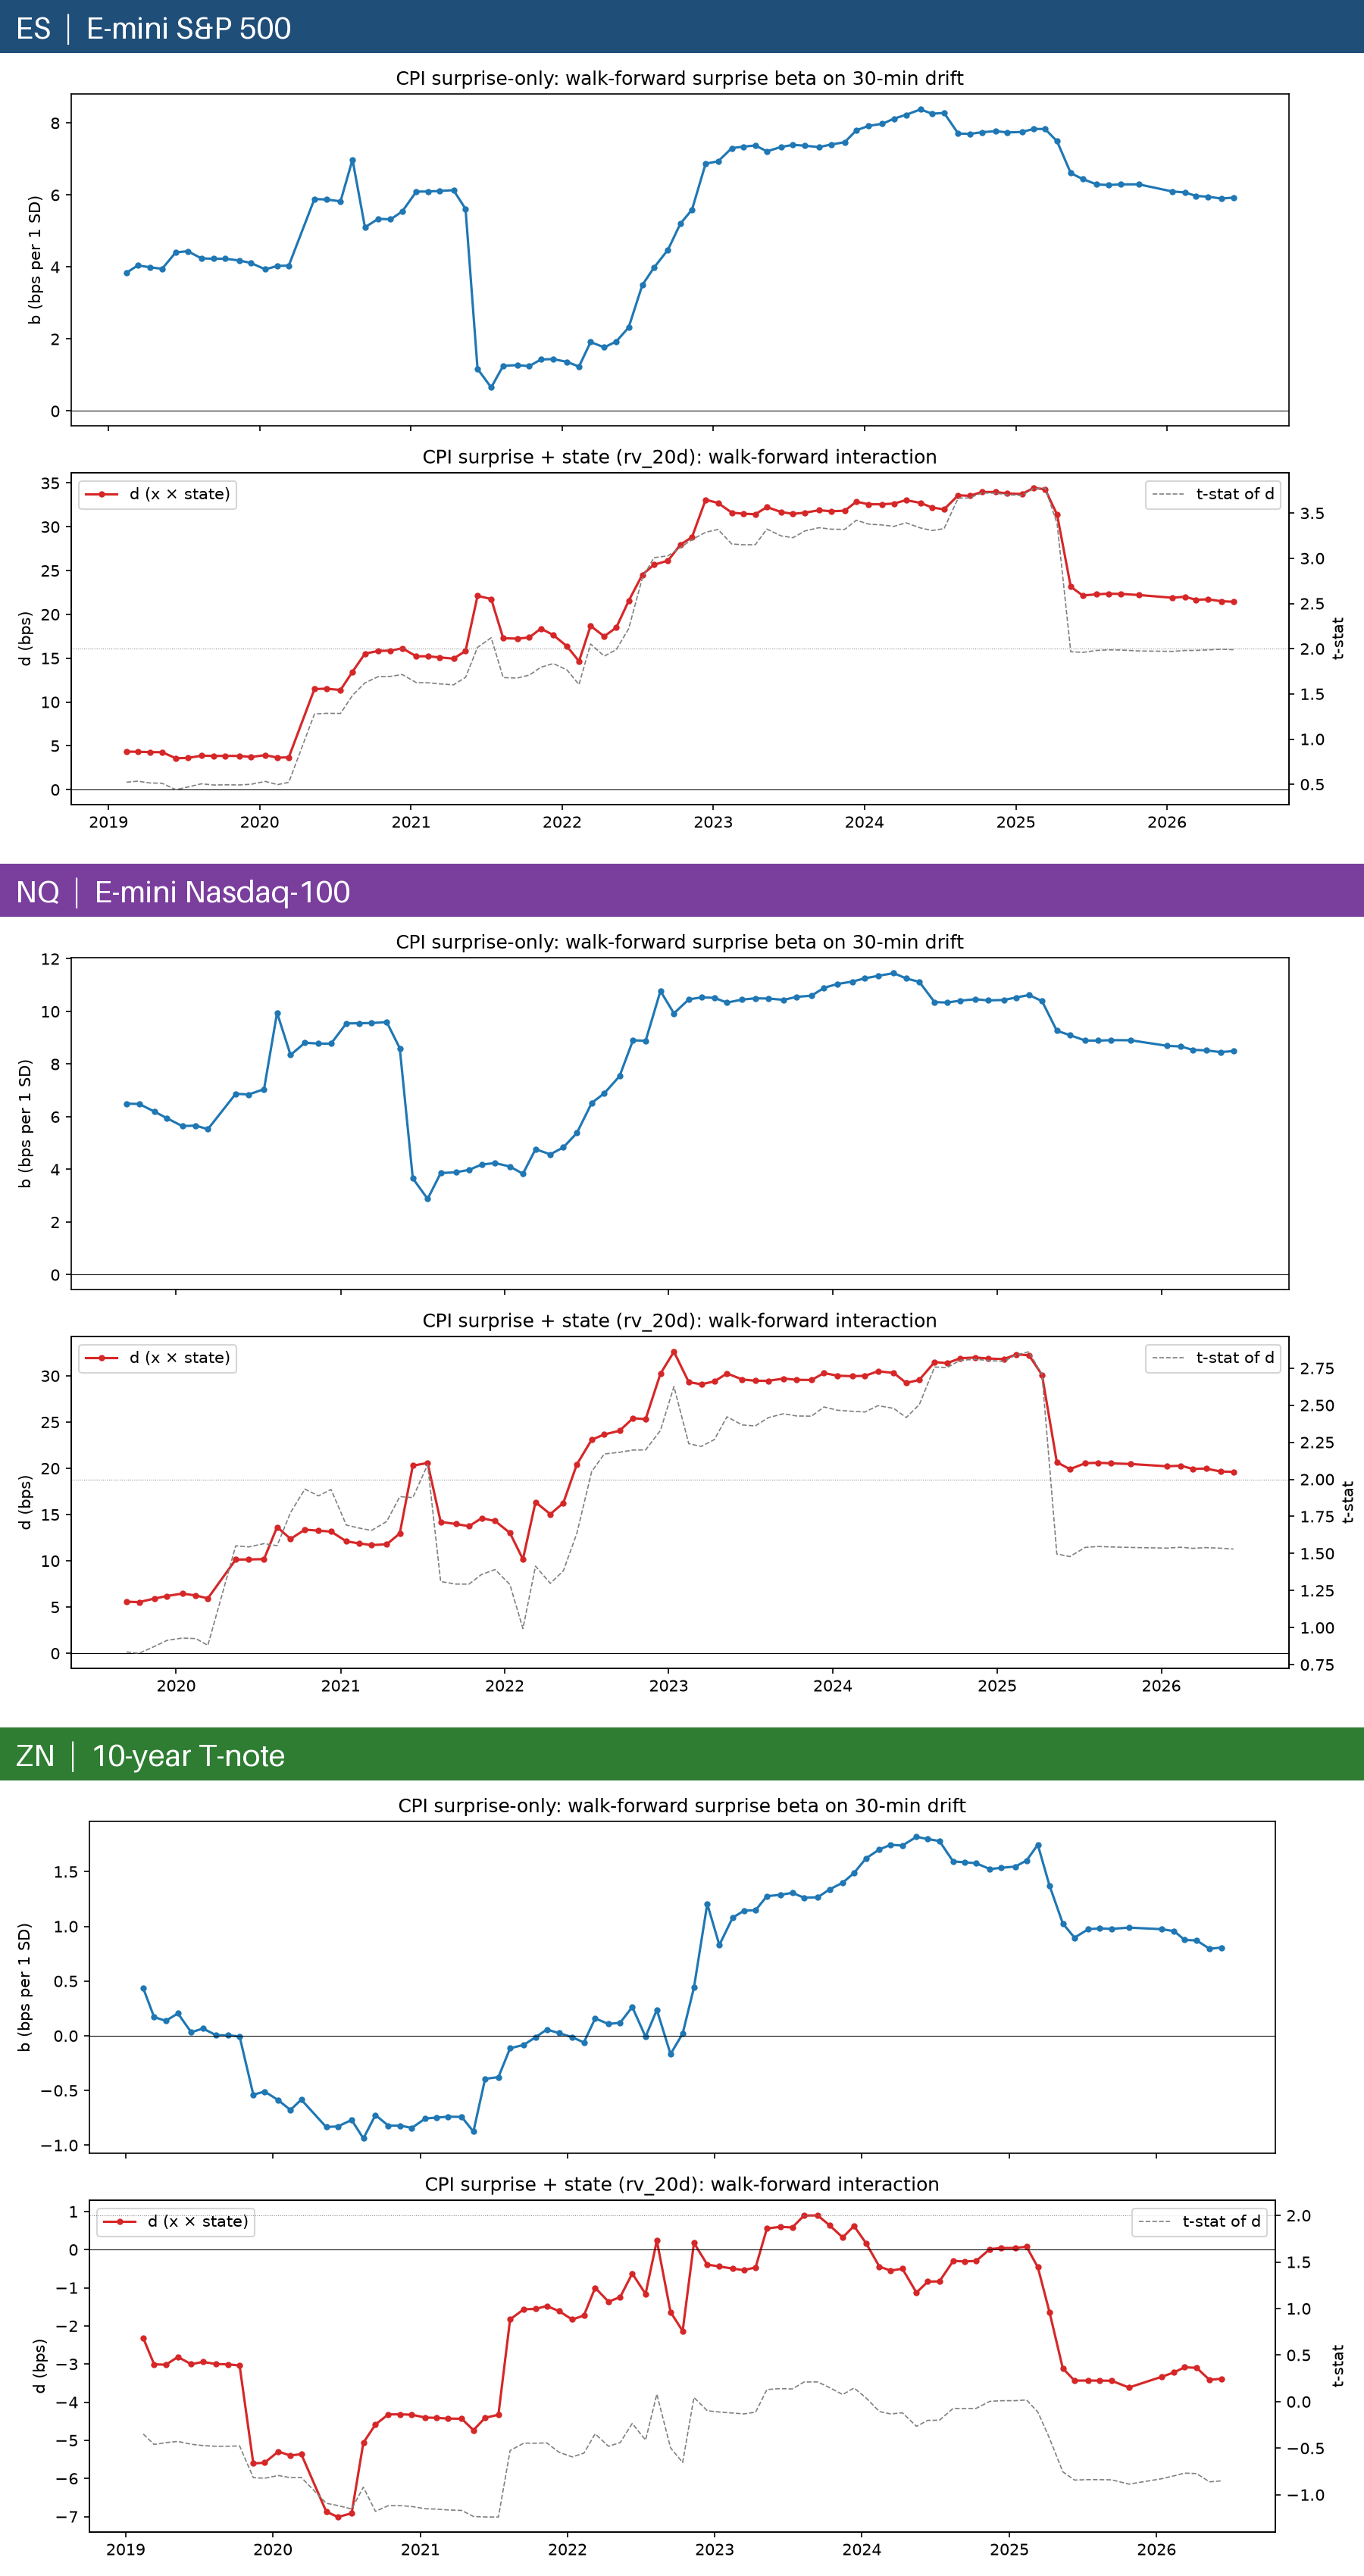
\includegraphics[width=0.62\linewidth]{app_fig17_coefficient_paths_3markets}
  \caption{Walk-forward estimates for CPI, re-estimated before each release: the surprise slope and
  the surprise $\times$ 20-day volatility interaction with their $t$-statistics, \ES, \NQ\ and \ZN.}
  \label{fig:app_paths}
\end{figure}

\begin{figure}[!htb]
  \centering
  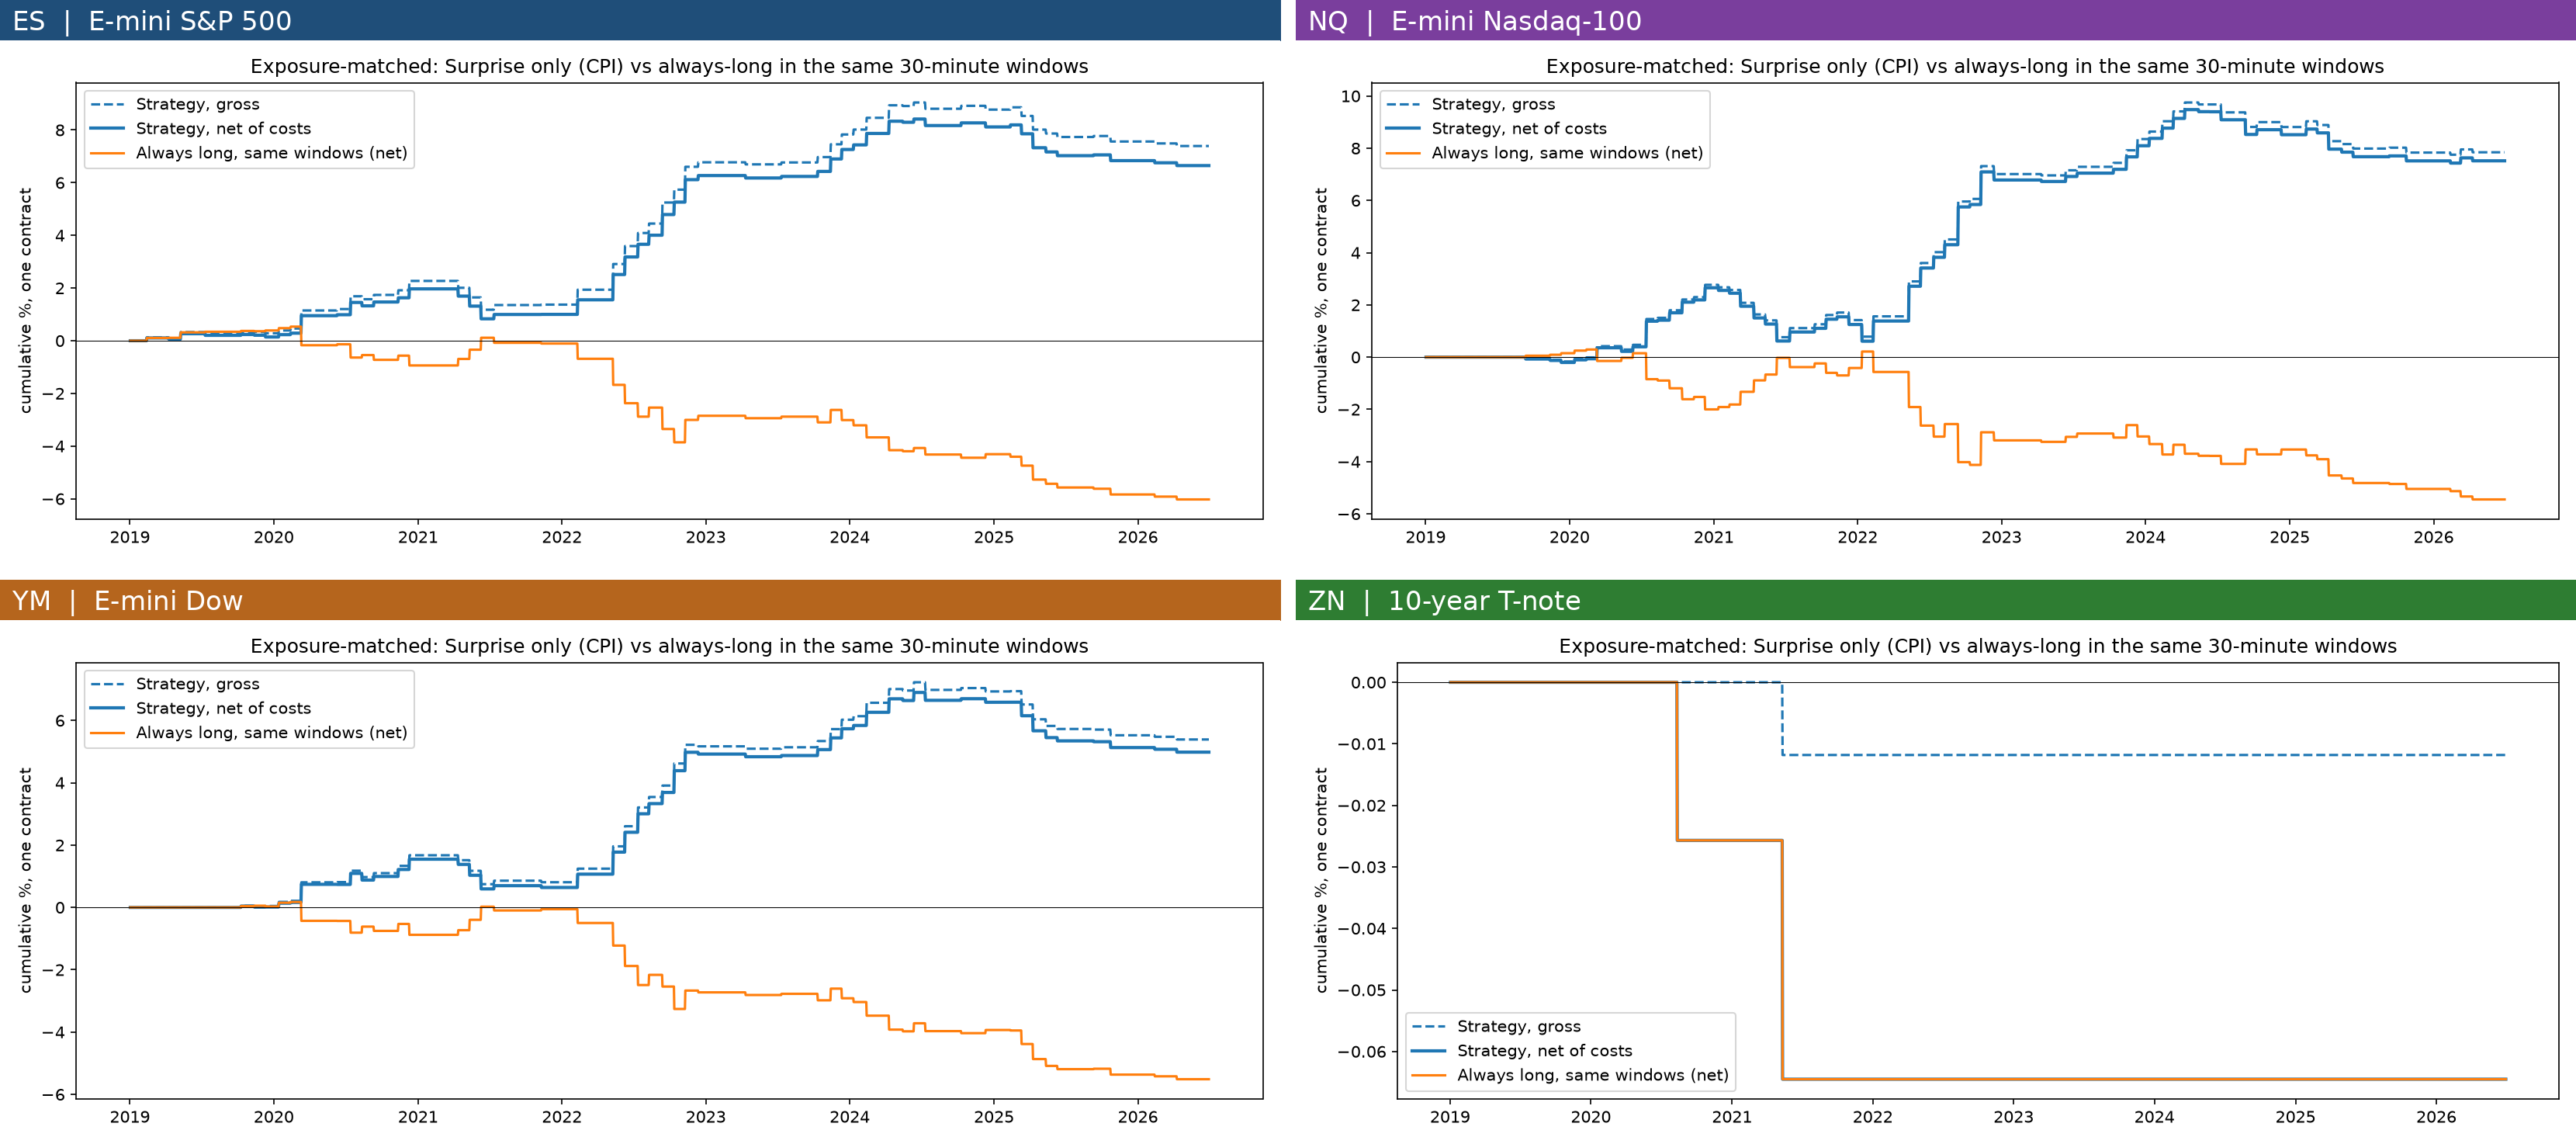
\includegraphics[width=\linewidth]{app_peer_CPI_surprise_only_4markets}
  \caption{Peer chart format, CPI surprise model, 2019--2026: cumulative return of one contract,
  gross and net of costs, against always long in the same windows.}
  \label{fig:app_peer}
\end{figure}

\begin{figure}[!htb]
  \centering
  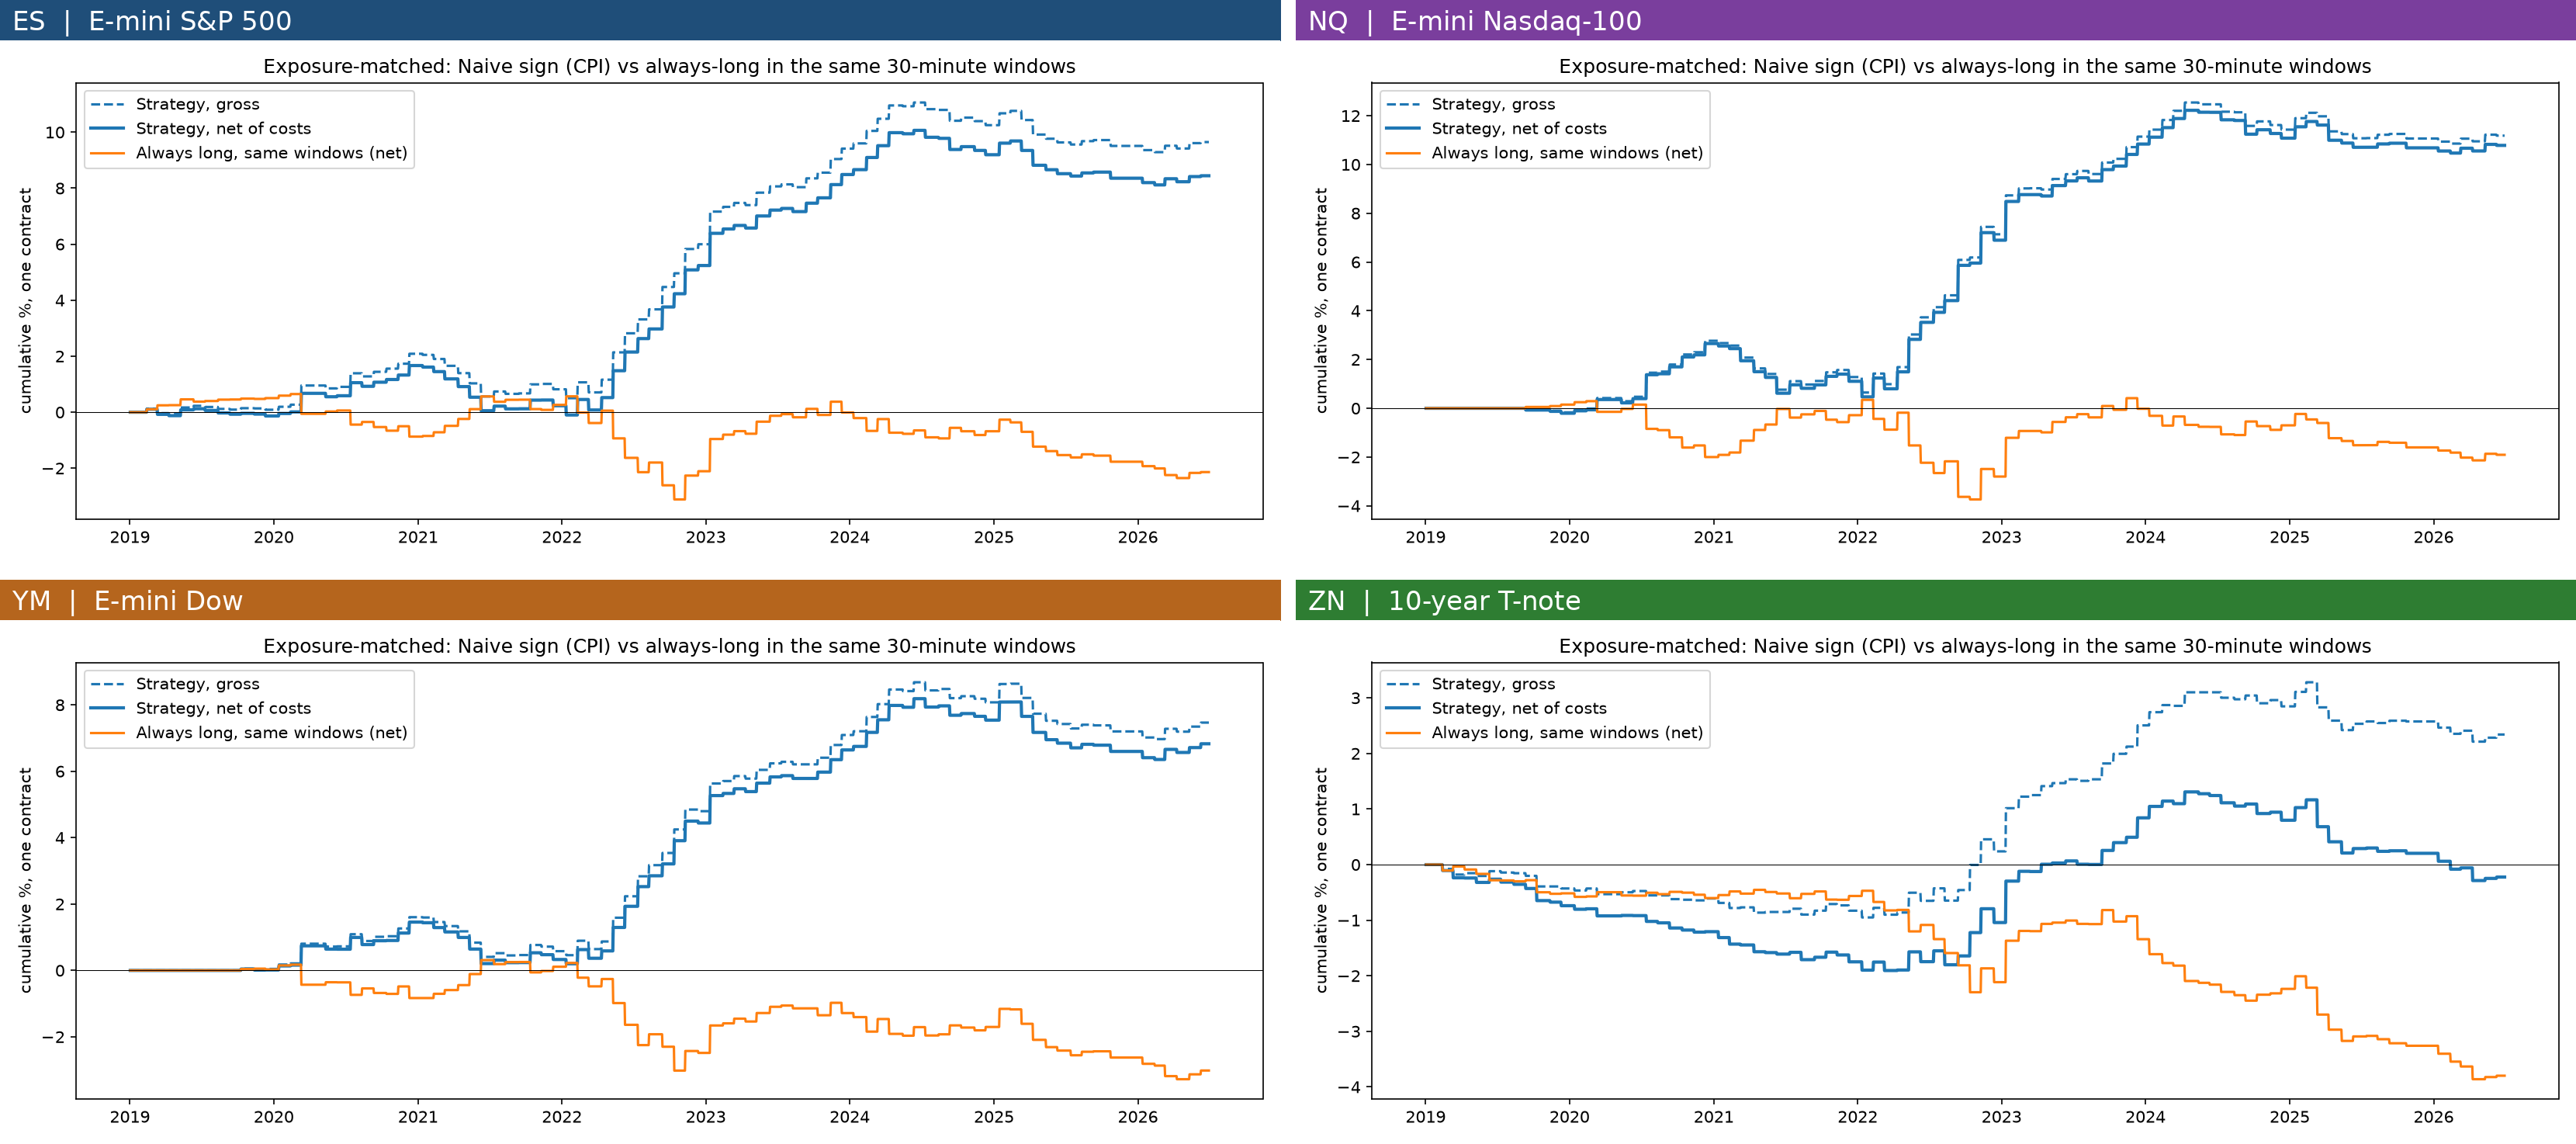
\includegraphics[width=\linewidth]{app_peer_CPI_naive_4markets}
  \caption{Peer chart format, CPI naive sign rule (every CPI release, sign of the headline
  surprise), 2019--2026.}
  \label{fig:app_peer_naive}
\end{figure}

\begin{figure}[!htb]
  \centering
  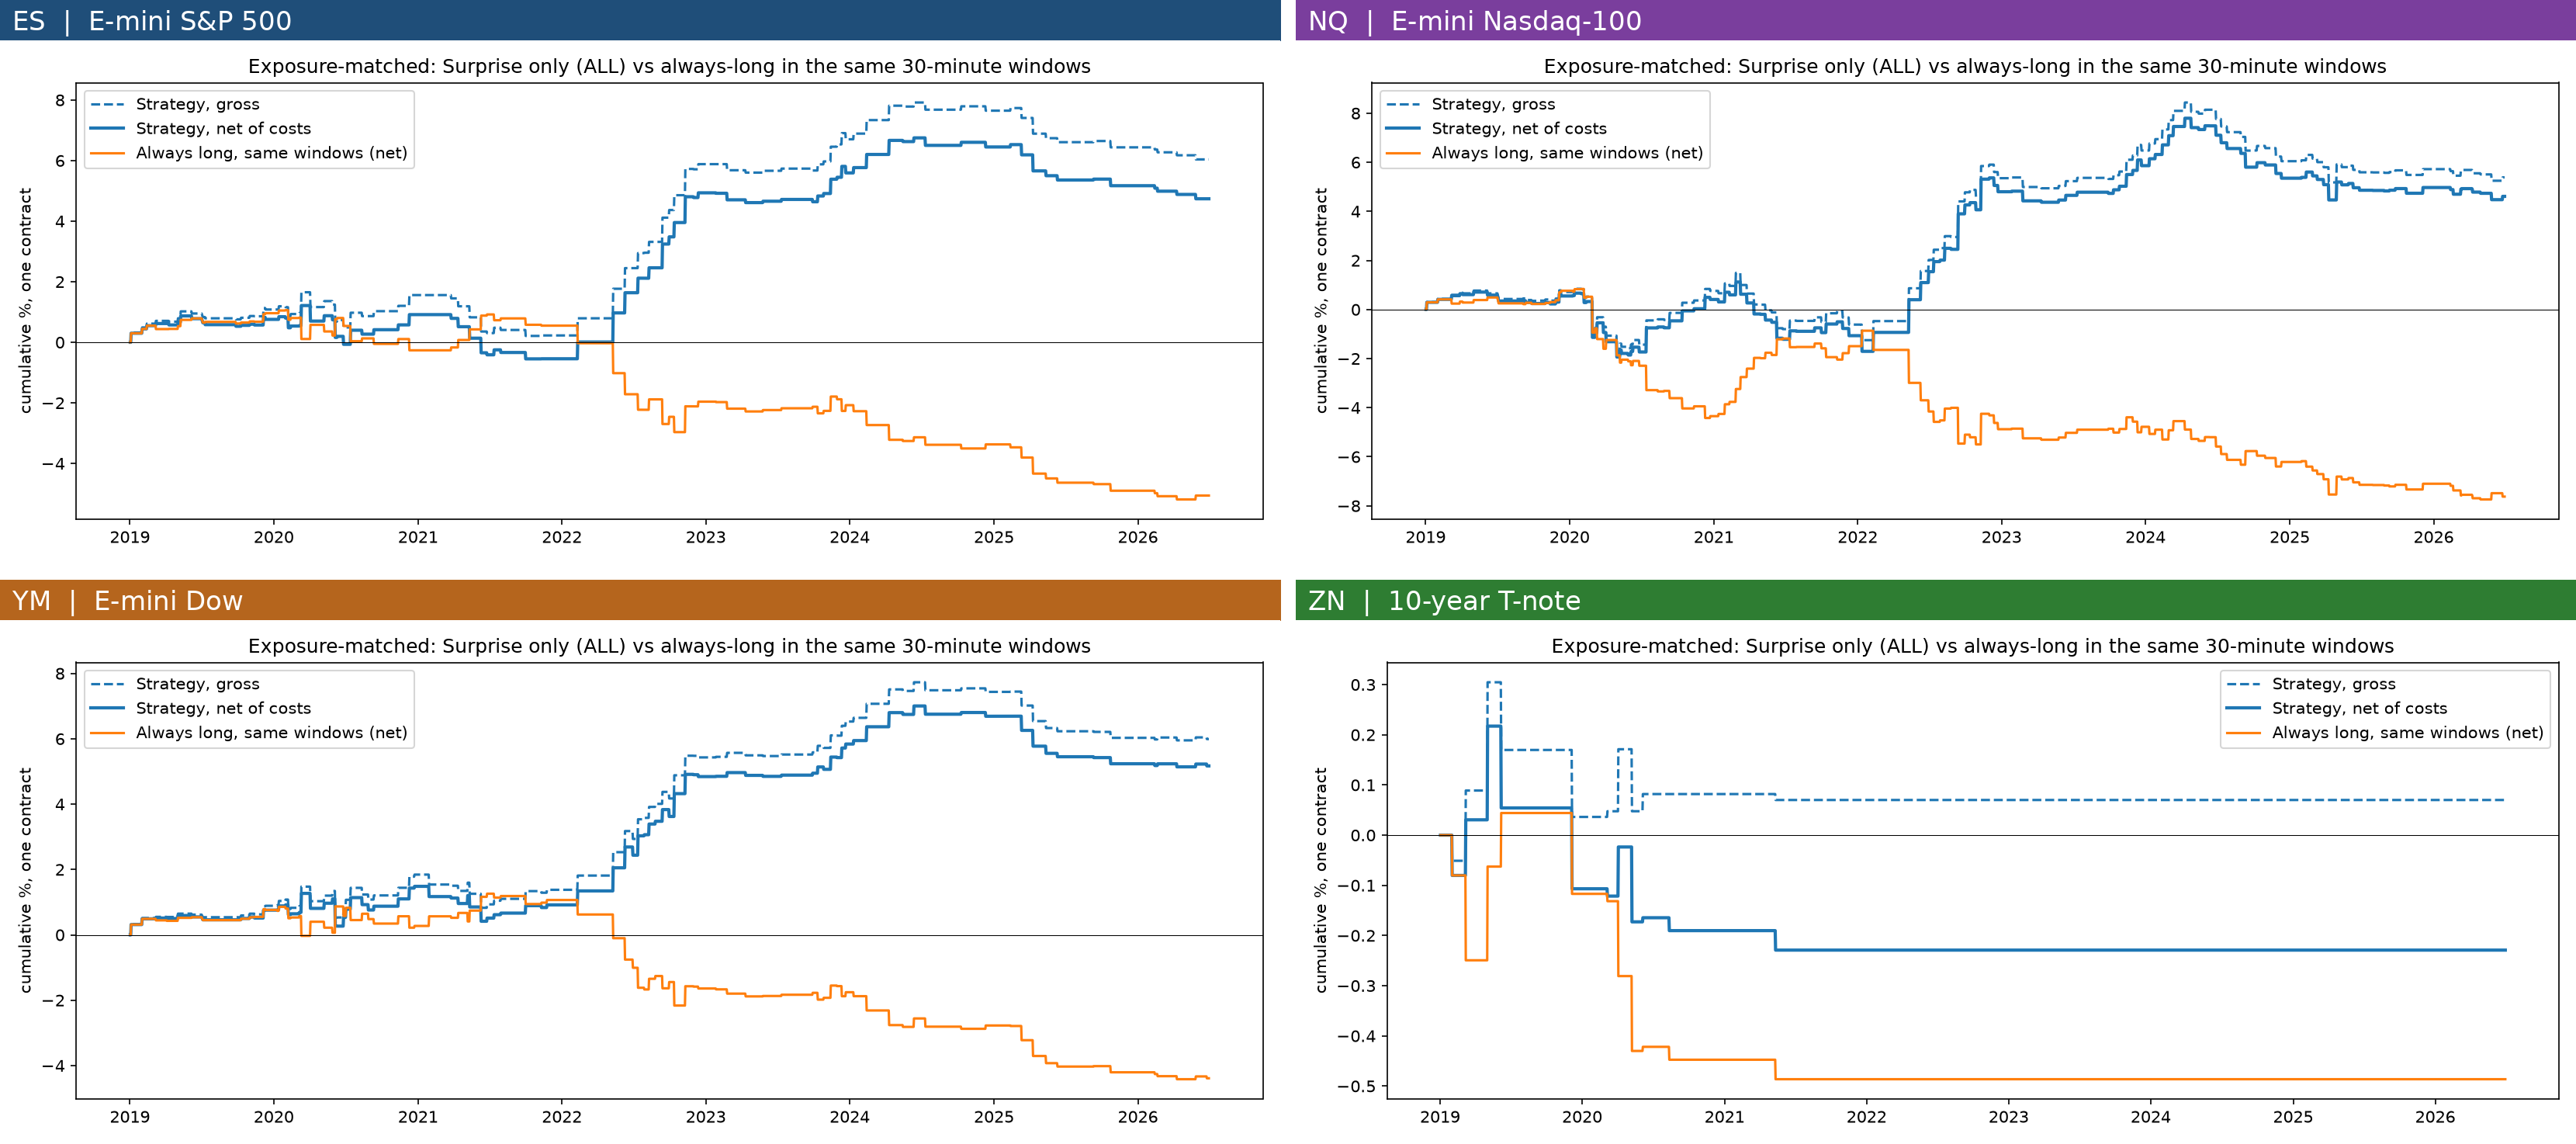
\includegraphics[width=\linewidth]{app_peer_ALL_surprise_only_4markets}
  \caption{Peer chart format, surprise model on CPI, PCE and payrolls, 2019--2026.}
  \label{fig:app_peer_all}
\end{figure}

\paragraph{Final comparison.} Table~\ref{tab:app_final} and Figure~\ref{fig:app_final} compare
the five CPI strategies of notebook 04 (section 14) in all four markets and three release
universes. In the equity indices every CPI strategy has a positive Sharpe ratio, and the naive
sign rule is the best or close to it (1.03 in \ES, 1.00 in \NQ, 0.99 in \YM); conditioning on the
pre-release state never improves on the surprise alone by a significant margin (the smallest
bootstrap probability that a state model is not better is 0.23). Adding PCE and payrolls lowers the
naive rule in \ES\ and \NQ\ but less so in \YM. In \ZN\ the fitted models almost never trade,
because their predicted drift rarely exceeds one tick, and every strategy is negative.

\begin{table}[!htb]
  \centering\small
  \caption{Walk-forward CPI strategies, net Sharpe ratio (90\% block-bootstrap interval), 2019--2026,
  2 ticks + \$4.50.}\label{tab:app_final}
  \begin{threeparttable}
  \setlength{\tabcolsep}{4pt}
  \begin{tabular}{lcccc}
    \toprule
    Strategy & \ES & \NQ & \YM & \ZN \\
    \midrule
    \multicolumn{5}{l}{\emph{CPI only}} \\
    Naive sign & 1.03 [0.32, 1.76] & 1.00 [0.37, 1.66] & 0.99 [0.27, 1.72] & $-0.05$ [$-0.82$, 0.56] \\
    Surprise only & 0.99 [0.25, 1.72] & 0.79 [0.12, 1.47] & 0.84 [0.07, 1.61] & $-0.51$ (2 trades) \\
    Surprise + State & 0.77 [0.01, 1.51] & 0.75 [0.04, 1.44] & 0.83 [0.13, 1.51] & $-0.40$ (5 trades) \\
    Surprise + State filter & 1.07 [0.40, 1.67] & 0.82 [0.20, 1.38] & 0.98 [0.25, 1.65] & $-0.37$ (1 trade) \\
    Surprise + Adaptive state & 0.95 [0.26, 1.61] & 0.75 [0.04, 1.44] & 0.74 [0.02, 1.44] & $-0.51$ (2 trades) \\
    \midrule
    \multicolumn{5}{l}{\emph{CPI, PCE and payrolls}} \\
    Naive sign & 0.33 & 0.38 & 0.57 & $-0.65$ \\
    Surprise only & 0.59 & 0.37 & 0.78 & $-0.22$ \\
    Surprise + State filter & 0.65 & 0.37 & 0.81 & $-0.07$ \\
    \midrule
    CPI trades, naive / surprise only & 86 / 52 & 79 / 62 & 77 / 48 & 86 / 2 \\
    \bottomrule
  \end{tabular}
  \begin{tablenotes}\footnotesize
    \item Notes: Entry at $T+1$, exit at $T+30$; every slope, sign and state model re-estimated on
    earlier releases only. Intervals from a three-month block bootstrap.
  \end{tablenotes}
  \end{threeparttable}
\end{table}

\begin{figure}[!htb]
  \centering
  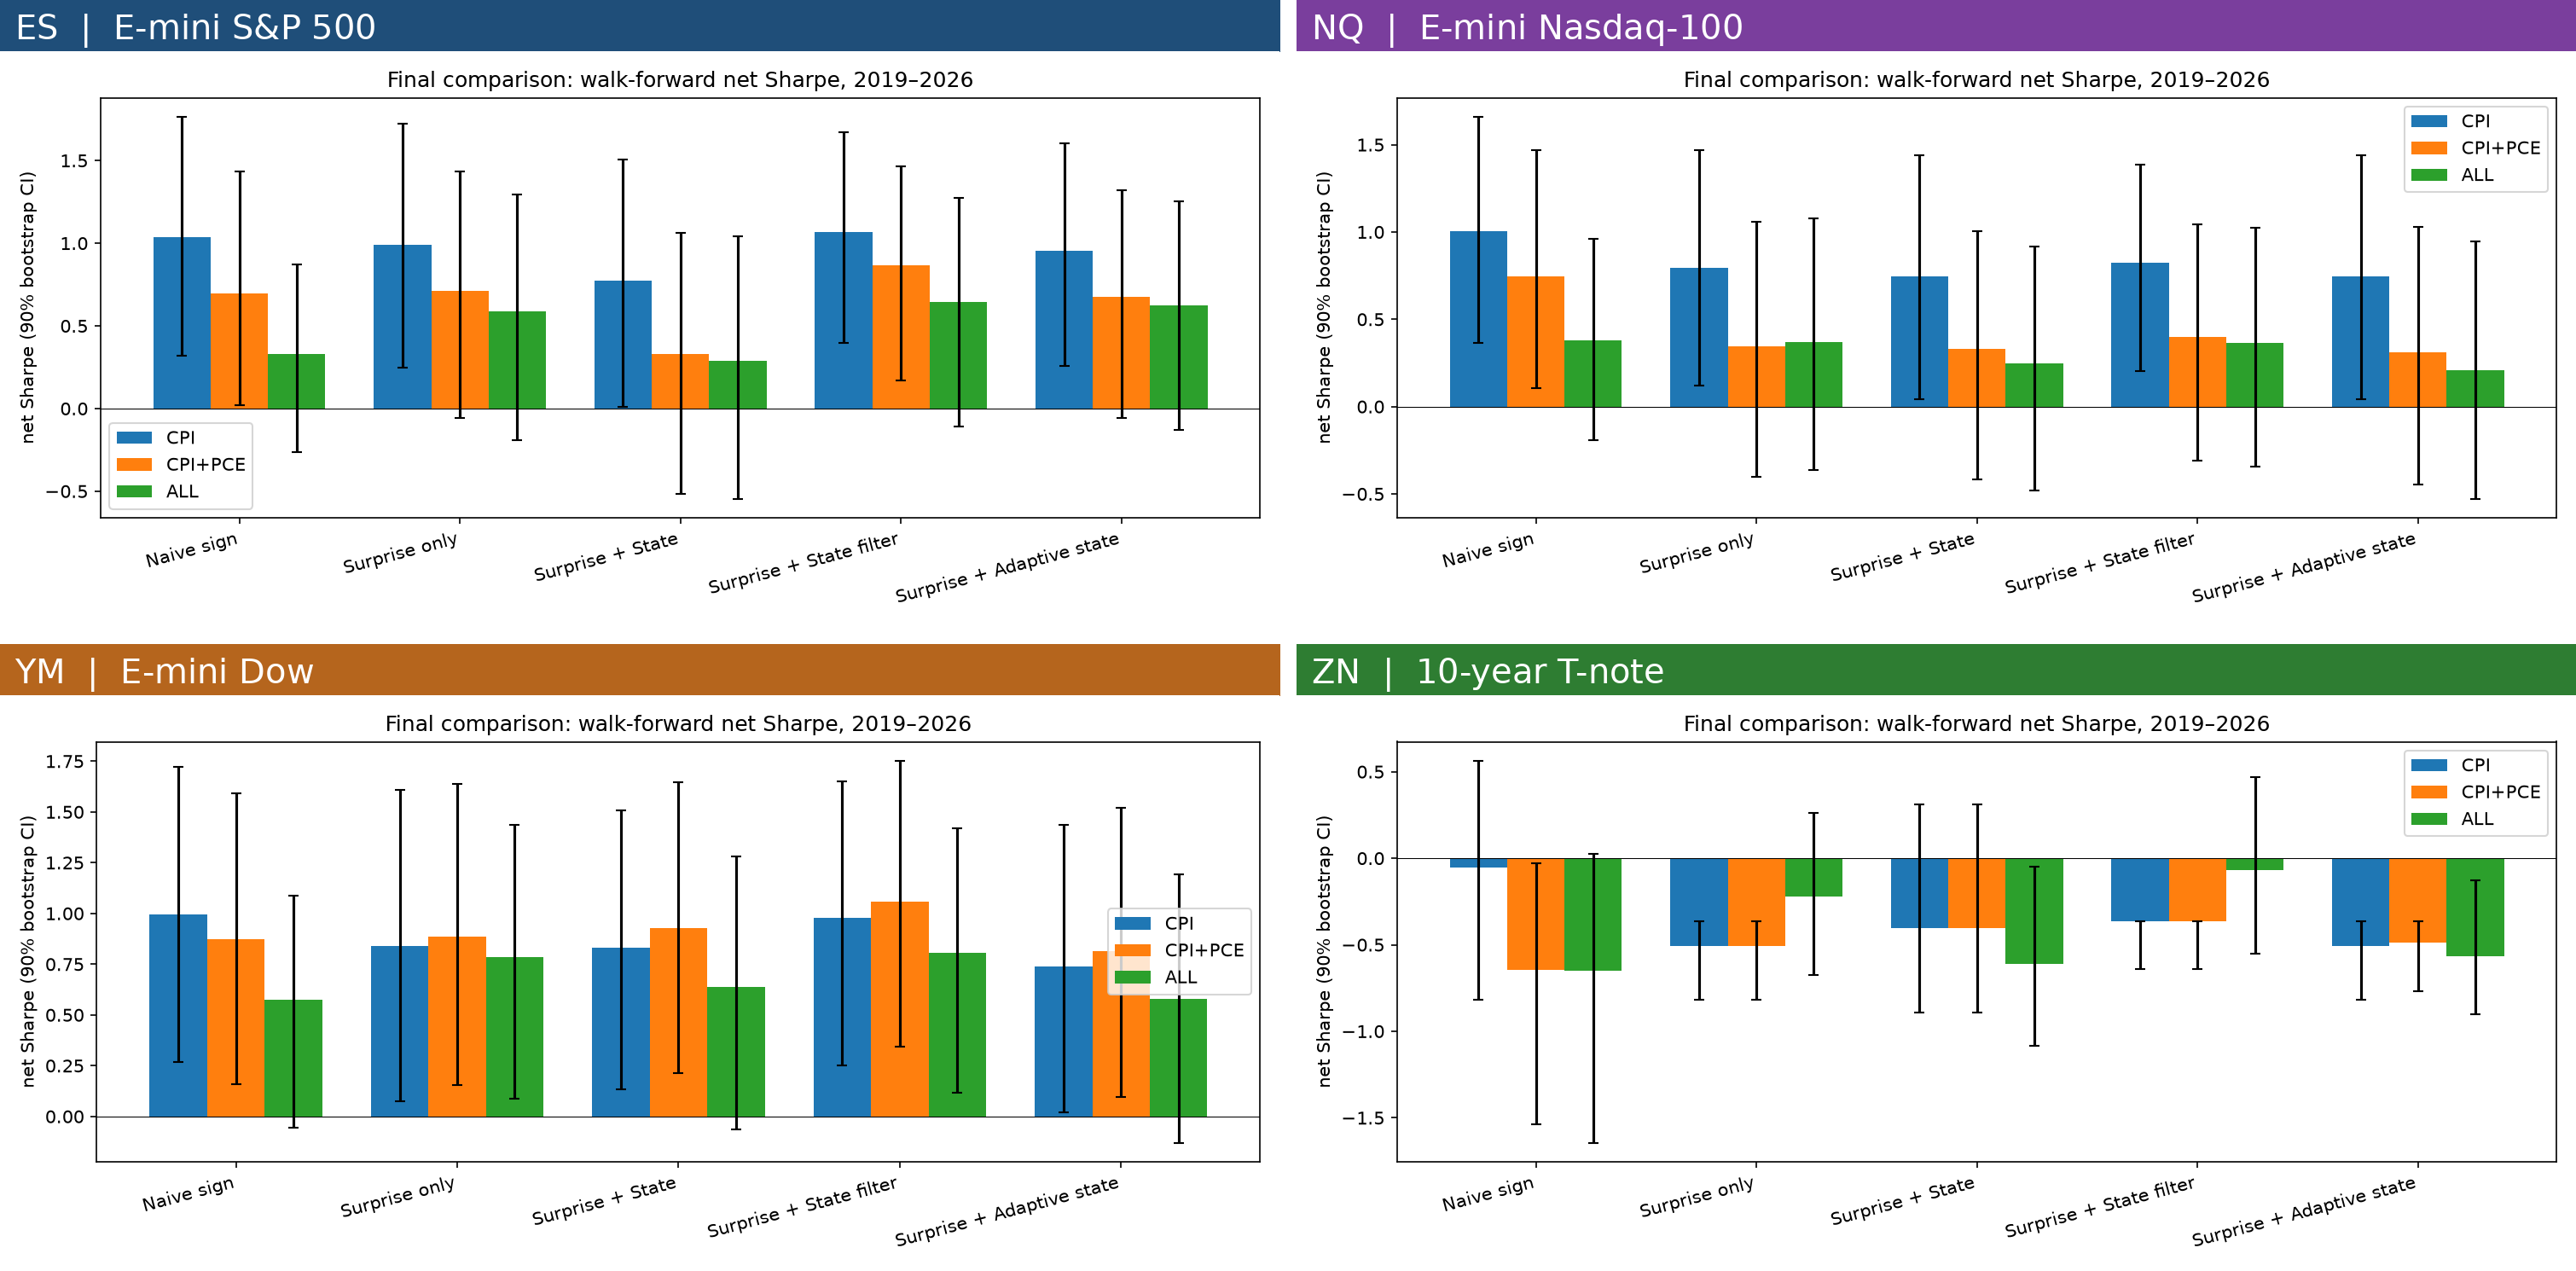
\includegraphics[width=\linewidth]{app_final_sharpe_4markets}
  \caption{Final comparison of notebook 04: walk-forward net Sharpe ratio with 90\% bootstrap
  intervals by strategy and release universe (CPI; CPI + PCE; CPI + PCE + NFP), 2019--2026.}
  \label{fig:app_final}
\end{figure}

\FloatBarrier
\subsection{Broad surprise book (notebook 05)}

\paragraph{Which releases earn money? (notebook 05, section 9.2).} Table~\ref{tab:app_family} and
Figure~\ref{fig:app_family} split the broad book's net P\&L (naive sizing, 2019--2026) by release
family. CPI is the largest contributor in every equity index: $+4.3\%$ of notional in \ES, $+6.0\%$
in \NQ\ and $+3.8\%$ in \YM. Behind it the ranking differs by market. In \ES\ the next contributors are
JOLTS ($+3.0\%$), retail sales ($+2.3\%$) and the University of Michigan survey ($+1.4\%$); in \NQ\
factory orders ($+4.6\%$), the University of Michigan survey ($+4.2\%$), retail sales ($+2.6\%$) and
GDP ($+2.1\%$); in \YM\ ISM Manufacturing ($+3.3\%$), JOLTS ($+2.3\%$) and retail sales ($+1.7\%$).
Payrolls, the release with the largest market impact, earns nothing or loses in all three ($-1.7\%$,
$-0.5\%$ and $-0.1\%$), and ISM Services, the regional Fed surveys and pending home sales lose small
amounts. No major family is individually significant: the $t$-statistics of the main families are at
most 1.9 with naive sizing, and CPI with volatility sizing reaches 2.0 in \ES\ and 1.9 in \NQ. The broad book
therefore works through diversification across many small edges rather than through one release.
In \ZN\ every family with more than a handful of trades loses, led by payrolls ($-4.9\%$), retail
sales ($-4.5\%$) and CPI ($-3.0\%$): its hit rates of 22--47\% reflect a drift smaller than the cost.

\begin{table}[!htb]
  \centering\small
  \caption{Net P\&L of the broad surprise book by release family, 2019--2026: total net return
  (\% of notional) and $t$-statistic of the mean trade, naive sizing.}\label{tab:app_family}
  \begin{threeparttable}
  \setlength{\tabcolsep}{3pt}
  \begin{tabular}{lcclcclcc}
    \toprule
    \multicolumn{3}{c}{\ES} & \multicolumn{3}{c}{\NQ} & \multicolumn{3}{c}{\YM} \\
    \cmidrule(lr){1-3}\cmidrule(lr){4-6}\cmidrule(lr){7-9}
    Family & Total & $t$ & Family & Total & $t$ & Family & Total & $t$ \\
    \midrule
    CPI & 4.3\% & 1.40 & CPI & 6.0\% & 1.50 & CPI & 3.8\% & 1.48 \\
    JOLTS & 3.0\% & 1.56 & Factory Orders & 4.6\% & 1.89 & ISM Manuf. & 3.3\% & 1.02 \\
    Retail Sales & 2.3\% & 1.12 & U.\ of Michigan & 4.2\% & 1.45 & JOLTS & 2.3\% & 1.19 \\
    U.\ of Michigan & 1.4\% & 0.67 & Retail Sales & 2.6\% & 1.13 & Retail Sales & 1.7\% & 1.01 \\
    Adv.\ Goods Trade & 1.3\% & 1.13 & GDP & 2.1\% & 1.55 & Trade Balance & 1.2\% & 0.88 \\
    \midrule
    ISM Services & $-1.5\%$ & $-0.49$ & ISM Services & $-1.3\%$ & $-0.32$ & Wholesale Trade & $-1.6\%$ & $-2.40$ \\
    Payrolls (NFP) & $-1.7\%$ & $-0.60$ & Richmond Fed & $-1.9\%$ & $-1.02$ & Wholesale Inv. & $-2.7\%$ & $-1.68$ \\
    \bottomrule
  \end{tabular}
  \begin{tablenotes}\footnotesize
    \item Notes: Top five contributors and the two largest losers in each market. Payrolls: $-0.5\%$
    in \NQ\ and $-0.1\%$ in \YM. In \ZN\ every family with more than a few trades loses.
  \end{tablenotes}
  \end{threeparttable}
\end{table}

\begin{figure}[!htb]
  \centering
  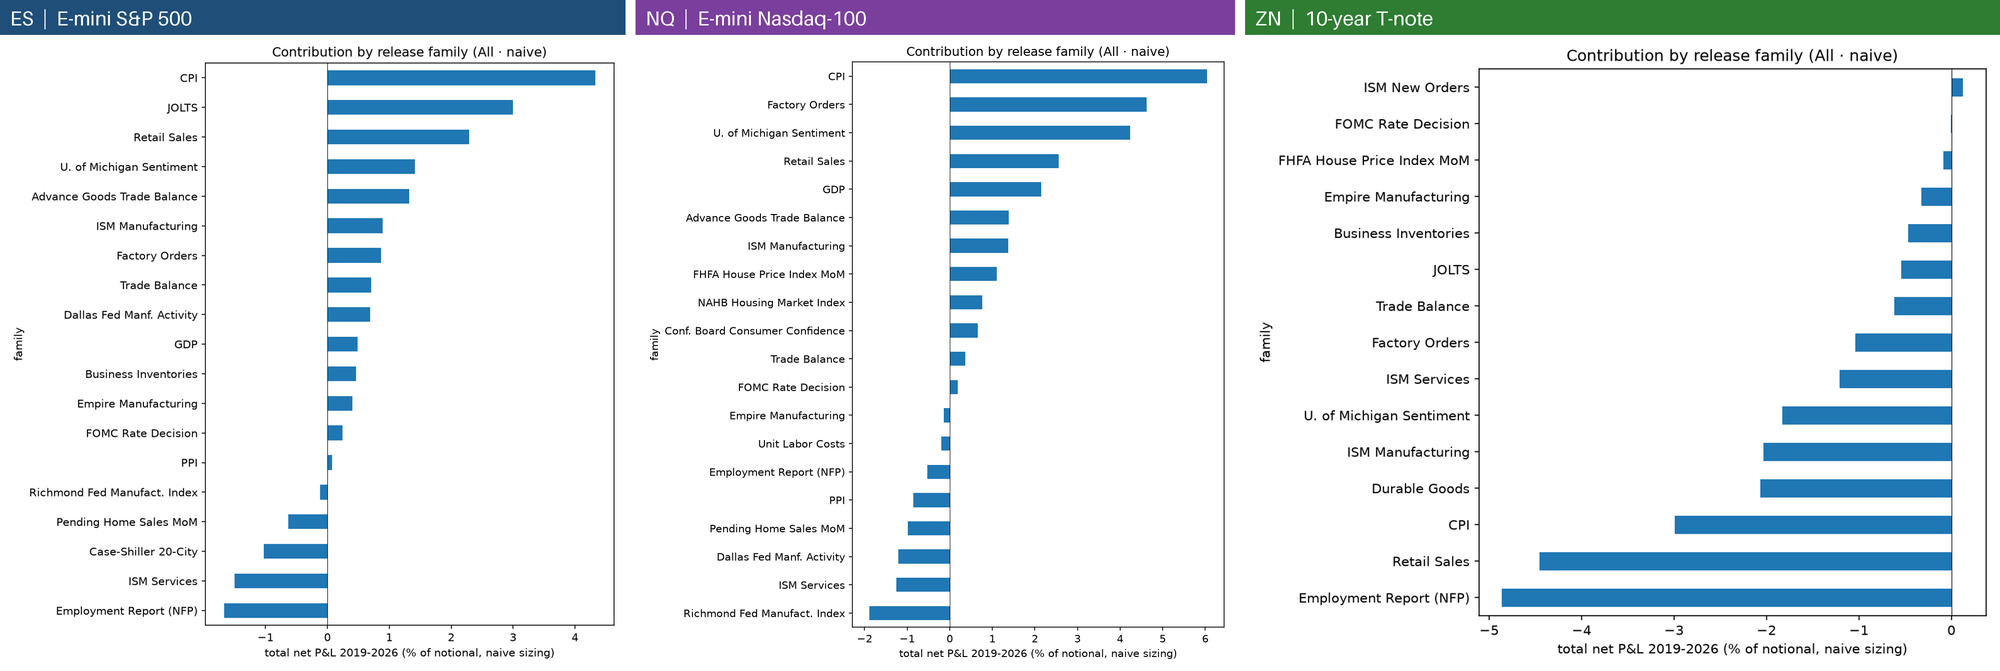
\includegraphics[width=\linewidth]{app_fig26_family_contribution_3markets}\\[4pt]
  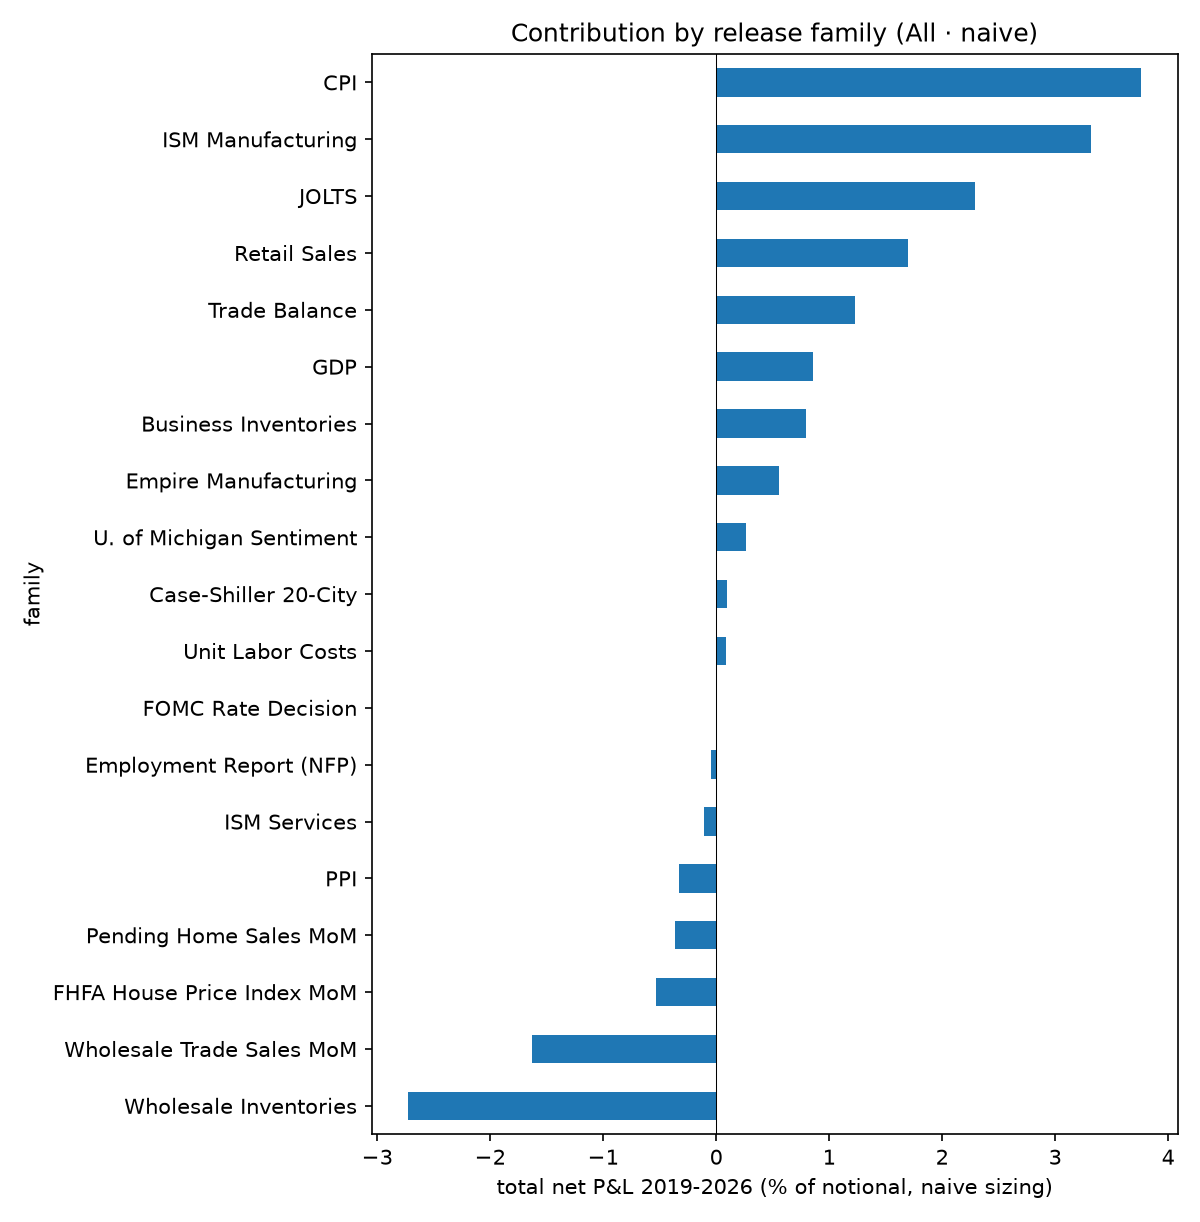
\includegraphics[width=0.42\linewidth]{app_nb05b_YM_family_contribution}
  \caption{Total net P\&L of the broad surprise book by release family, 2019--2026: \ES, \NQ\ and
  \ZN\ (top) and \YM\ (bottom).}
  \label{fig:app_family}
\end{figure}

\paragraph{CPI only against CPI plus other surprises (notebook 05, section 10).}
Figure~\ref{fig:app_nb05_final} and Table~\ref{tab:app_nb05_final} compare the CPI-only books (blue)
with the books that add the other screened releases (orange and green), against the DTW book from
the team's original slide (gray; \ES, 2018--2026, used as a fixed reference in every panel). The
trade-off is the same in every equity index. The CPI books earn the most per trade (5--16 bps net)
but trade only about 11 times a year. Adding the other releases raises the count to about 95 a year
at about 2 bps per trade, and the simple naive sign rule is then the best broad book (0.65 in \ES,
0.71 in \NQ, 0.68 in \YM), close to the CPI books' Sharpe ratio with far more trades, and it keeps the
highest Sharpe ratio without 2022 (0.28--0.44). The fitted surprise model and volatility scaling
help on CPI but not on the broad book, where scaling mainly adds drawdown ($-12$ to $-14\%$).
Trading a second 30-minute window doubles the trades and removes the edge. In \ZN\ every book
loses, and the fitted models almost never trade.

\begin{table}[!htb]
  \centering\small
  \caption{CPI only against CPI plus other surprises: net Sharpe ratio (trades per year),
  2019--2026, 2 ticks + \$4.50.}\label{tab:app_nb05_final}
  \begin{threeparttable}
  \setlength{\tabcolsep}{4pt}
  \begin{tabular}{lcccc}
    \toprule
    Book & \ES & \NQ & \YM & \ZN \\
    \midrule
    CPI $\cdot$ naive & 0.51 (12) & 0.54 (12) & 0.54 (11) & $-0.67$ (12) \\
    CPI $\cdot$ surprise model & 0.76 (9) & 0.55 (11) & 0.45 (9) & $-0.37$ (0) \\
    CPI $\cdot$ signal $\times$ vol & 0.77 (12) & 0.74 (12) & 0.61 (11) & $-0.29$ (12) \\
    \midrule
    All $\cdot$ naive & 0.65 (98) & 0.71 (97) & 0.68 (93) & $-2.42$ (82) \\
    All $\cdot$ surprise model & 0.11 (43) & 0.37 (66) & 0.34 (57) & $-0.74$ (2) \\
    All $\cdot$ signal $\times$ vol & 0.56 (101) & 0.37 (100) & 0.29 (96) & $-1.11$ (84) \\
    Combined (CPI model + others $\times$ vol) & 0.40 (98) & 0.23 (101) & 0.16 (95) & $-1.25$ (72) \\
    All $\cdot$ signal $\times$ vol $\cdot$ 2 windows & 0.16 (201) & 0.00 (199) & $-0.12$ (193) & $-2.02$ (168) \\
    \midrule
    All $\cdot$ naive, Sharpe without 2022 & 0.28 & 0.44 & 0.40 & $-2.53$ \\
    \bottomrule
  \end{tabular}
  \begin{tablenotes}\footnotesize
    \item Notes: CPI books use the average of all CPI lines as the signal, so the naive CPI rule
    differs from the headline-only rule of notebook 04. ``All'' is the ten screened families plus CPI.
  \end{tablenotes}
  \end{threeparttable}
\end{table}

\begin{figure}[!htb]
  \centering
  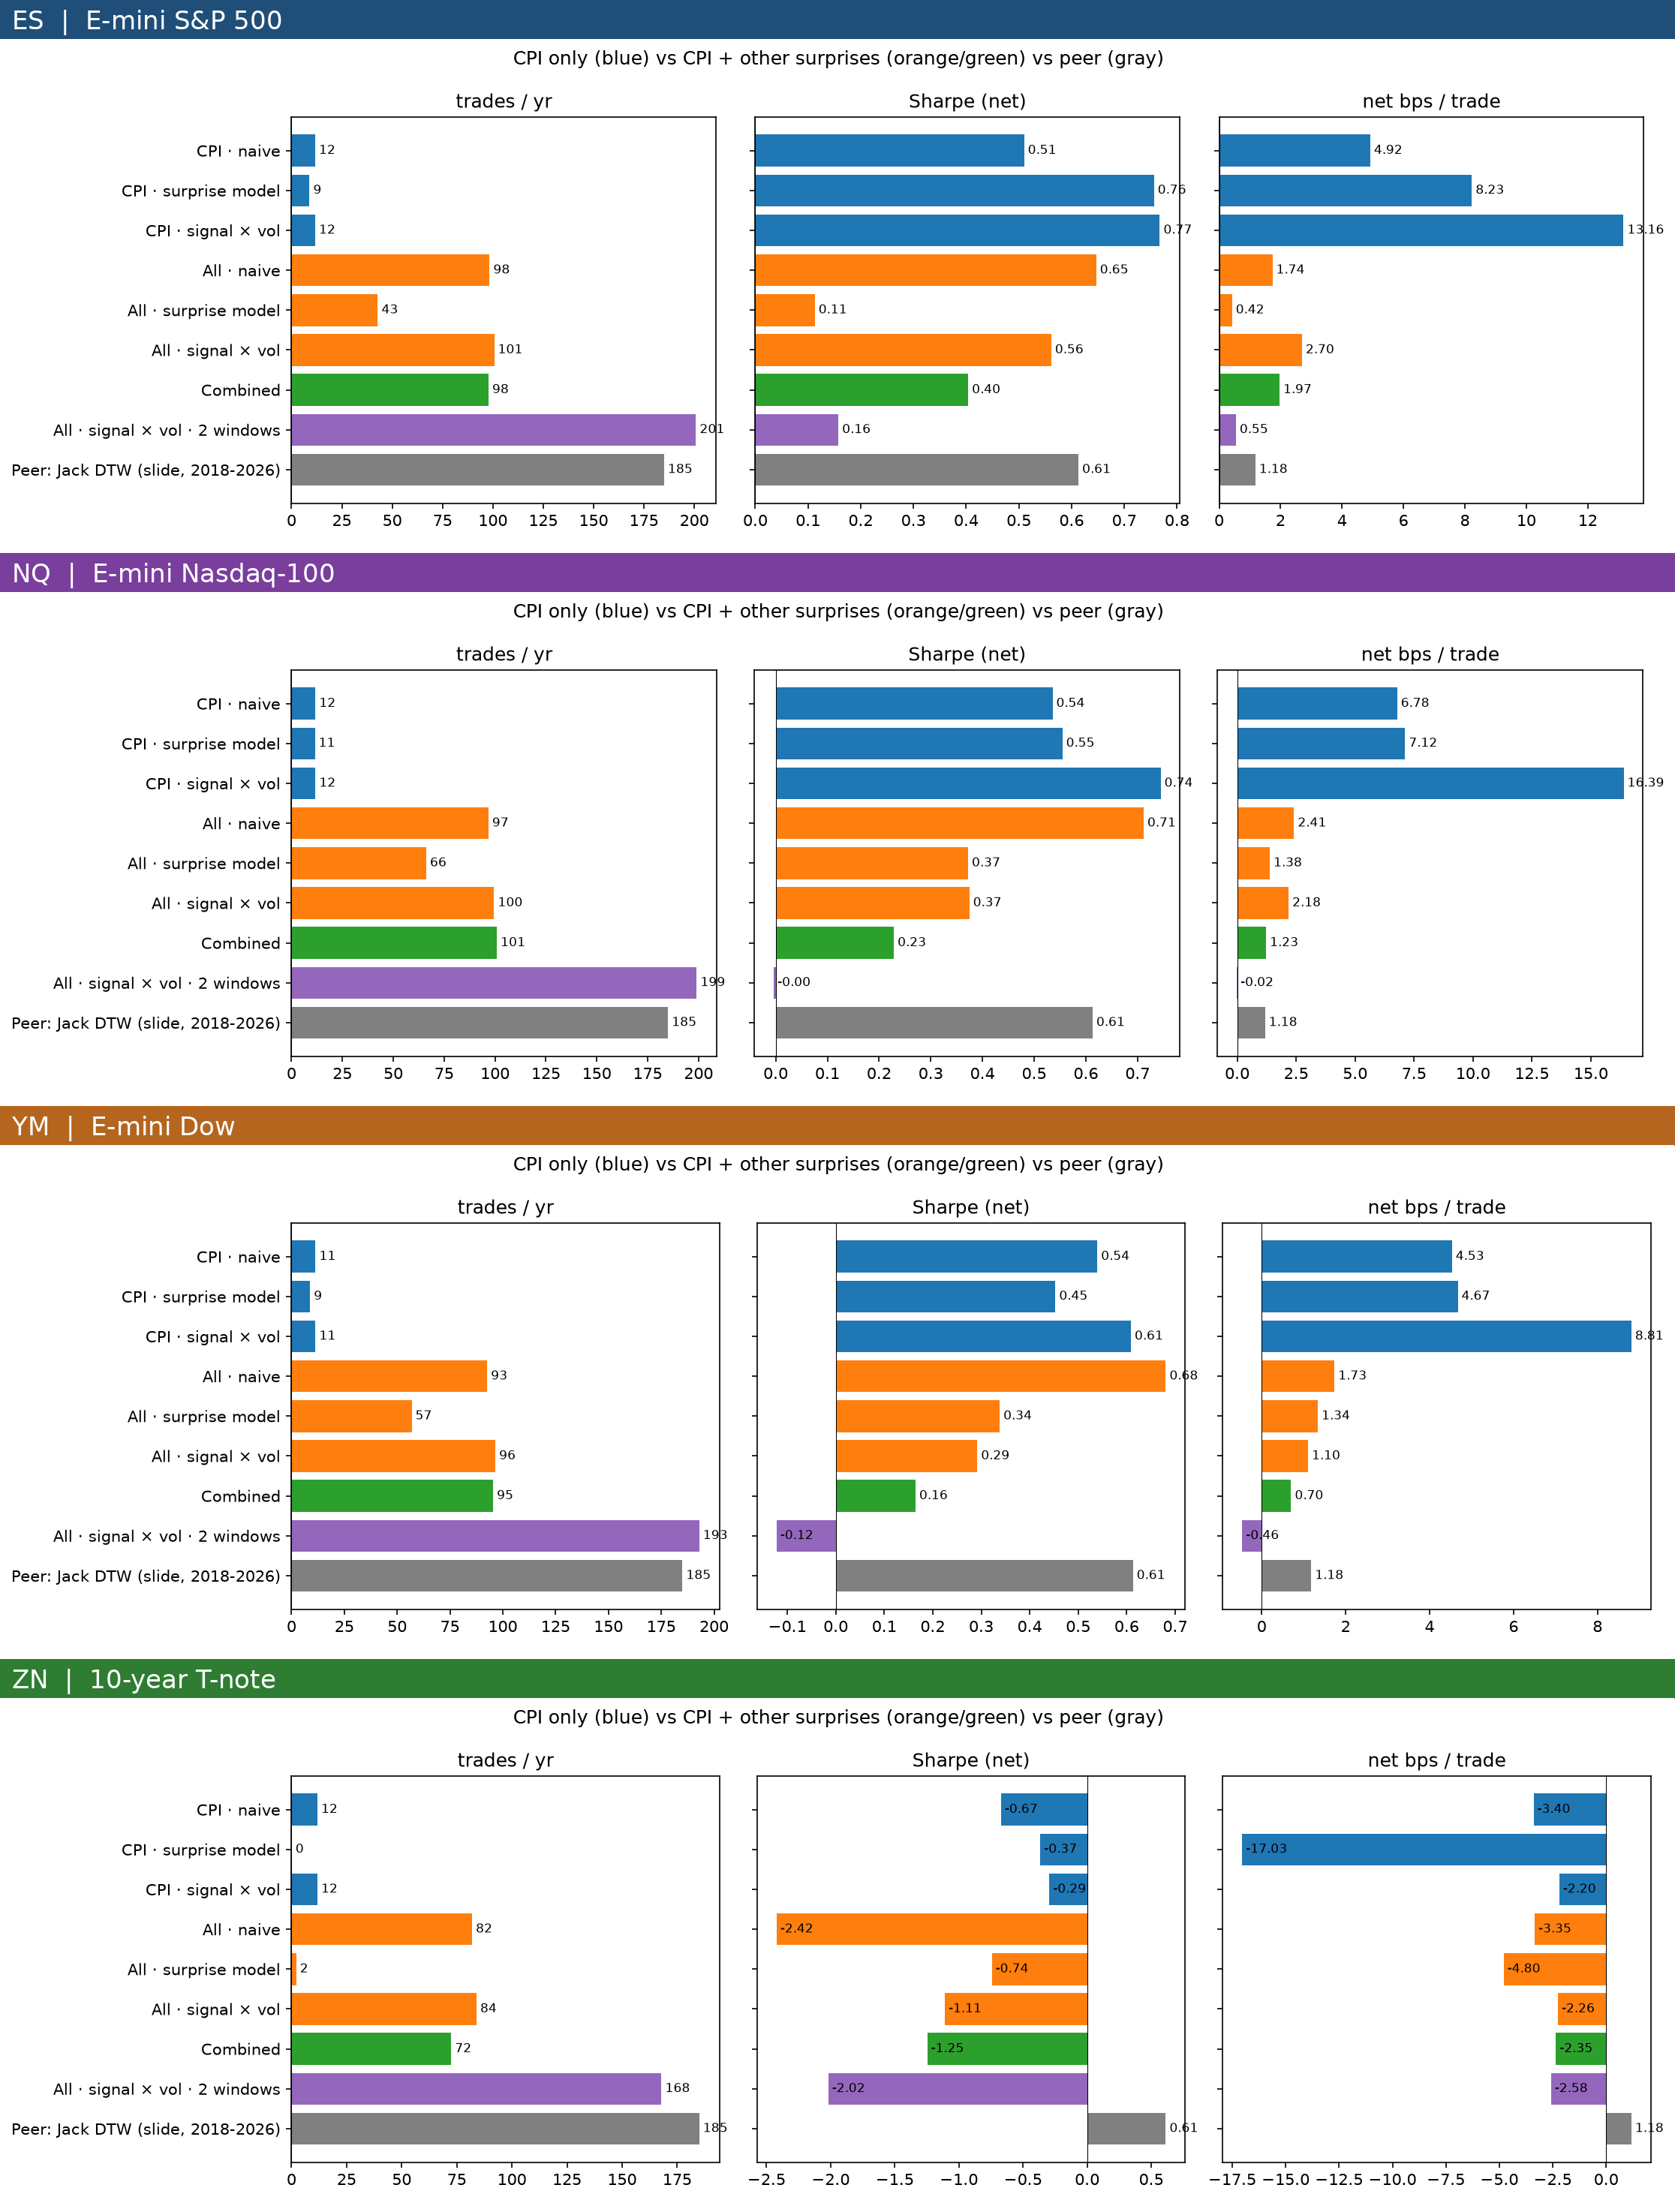
\includegraphics[width=0.85\linewidth]{app_nb05_final_comparison_4markets}
  \caption{CPI only (blue) against CPI plus other surprises (orange: ten screened families; green:
  CPI model plus volatility-scaled others; purple: two windows) and the DTW peer reference (gray):
  trades per year, net Sharpe ratio and net bps per trade, 2019--2026.}
  \label{fig:app_nb05_final}
\end{figure}

\FloatBarrier
\subsection{Surprise and DTW (notebook 06)}

\paragraph{Cumulative P\&L (notebook 06, section 7.3).} Figure~\ref{fig:app_nb06_cum} and
Table~\ref{tab:app_nb06} compare four single-window books on the same releases, walk-forward over
2019--2026 at our base cost: the surprise alone, the DTW direction alone, the surprise kept only when
DTW agrees, and a blend of the two signals. On the broad set of releases the surprise alone is the
best book in \ES\ (0.65) and \NQ\ (0.71); the DTW-only book loses in \ES\ and is flat in \NQ, and
requiring agreement removes about half the trades without raising the Sharpe ratio. \YM\ is the
exception: there DTW alone earns 0.47 and the blend 1.06, with a third of the drawdown, but the
bootstrap probability that the blend is not better than the surprise alone is 6\%, and the same
combination does not help in \ES\ or \NQ\ (Section~\ref{sec:results}). On CPI alone the four books are
close, and most of their cumulative P\&L comes from 2022. In \ZN\ every book loses; the
surprise book loses most because it trades every release and pays a full tick each time.

\begin{table}[!htb]
  \centering\small
  \caption{Surprise, DTW and combined single-window books: net Sharpe ratio, 2019--2026, 2 ticks +
  \$4.50.}\label{tab:app_nb06}
  \begin{tabular}{lcccc}
    \toprule
    Book & \ES & \NQ & \YM & \ZN \\
    \midrule
    \multicolumn{5}{l}{\emph{All screened releases}} \\
    Surprise only & 0.65 & 0.71 & 0.68 & $-2.42$ \\
    DTW only & $-0.39$ & 0.08 & 0.47 & $-1.25$ \\
    Surprise + DTW agree & 0.31 & 0.62 & 0.94 & $-1.57$ \\
    Surprise + DTW blend & 0.41 & 0.67 & 1.06 & $-1.51$ \\
    \midrule
    \multicolumn{5}{l}{\emph{CPI only}} \\
    Surprise only & 0.76 & 0.55 & 0.45 & $-0.37$ \\
    DTW only & 0.32 & 0.81 & 0.41 & $-0.55$ \\
    Surprise + DTW agree & 0.93 & 0.54 & 0.32 & -- \\
    Surprise + DTW blend & 0.69 & 0.72 & 0.51 & $-0.59$ \\
    \bottomrule
  \end{tabular}
  \par\smallskip\footnotesize ``--'': no trades. The \ZN\ CPI surprise book trades once.
\end{table}

\begin{figure}[!htb]
  \centering
  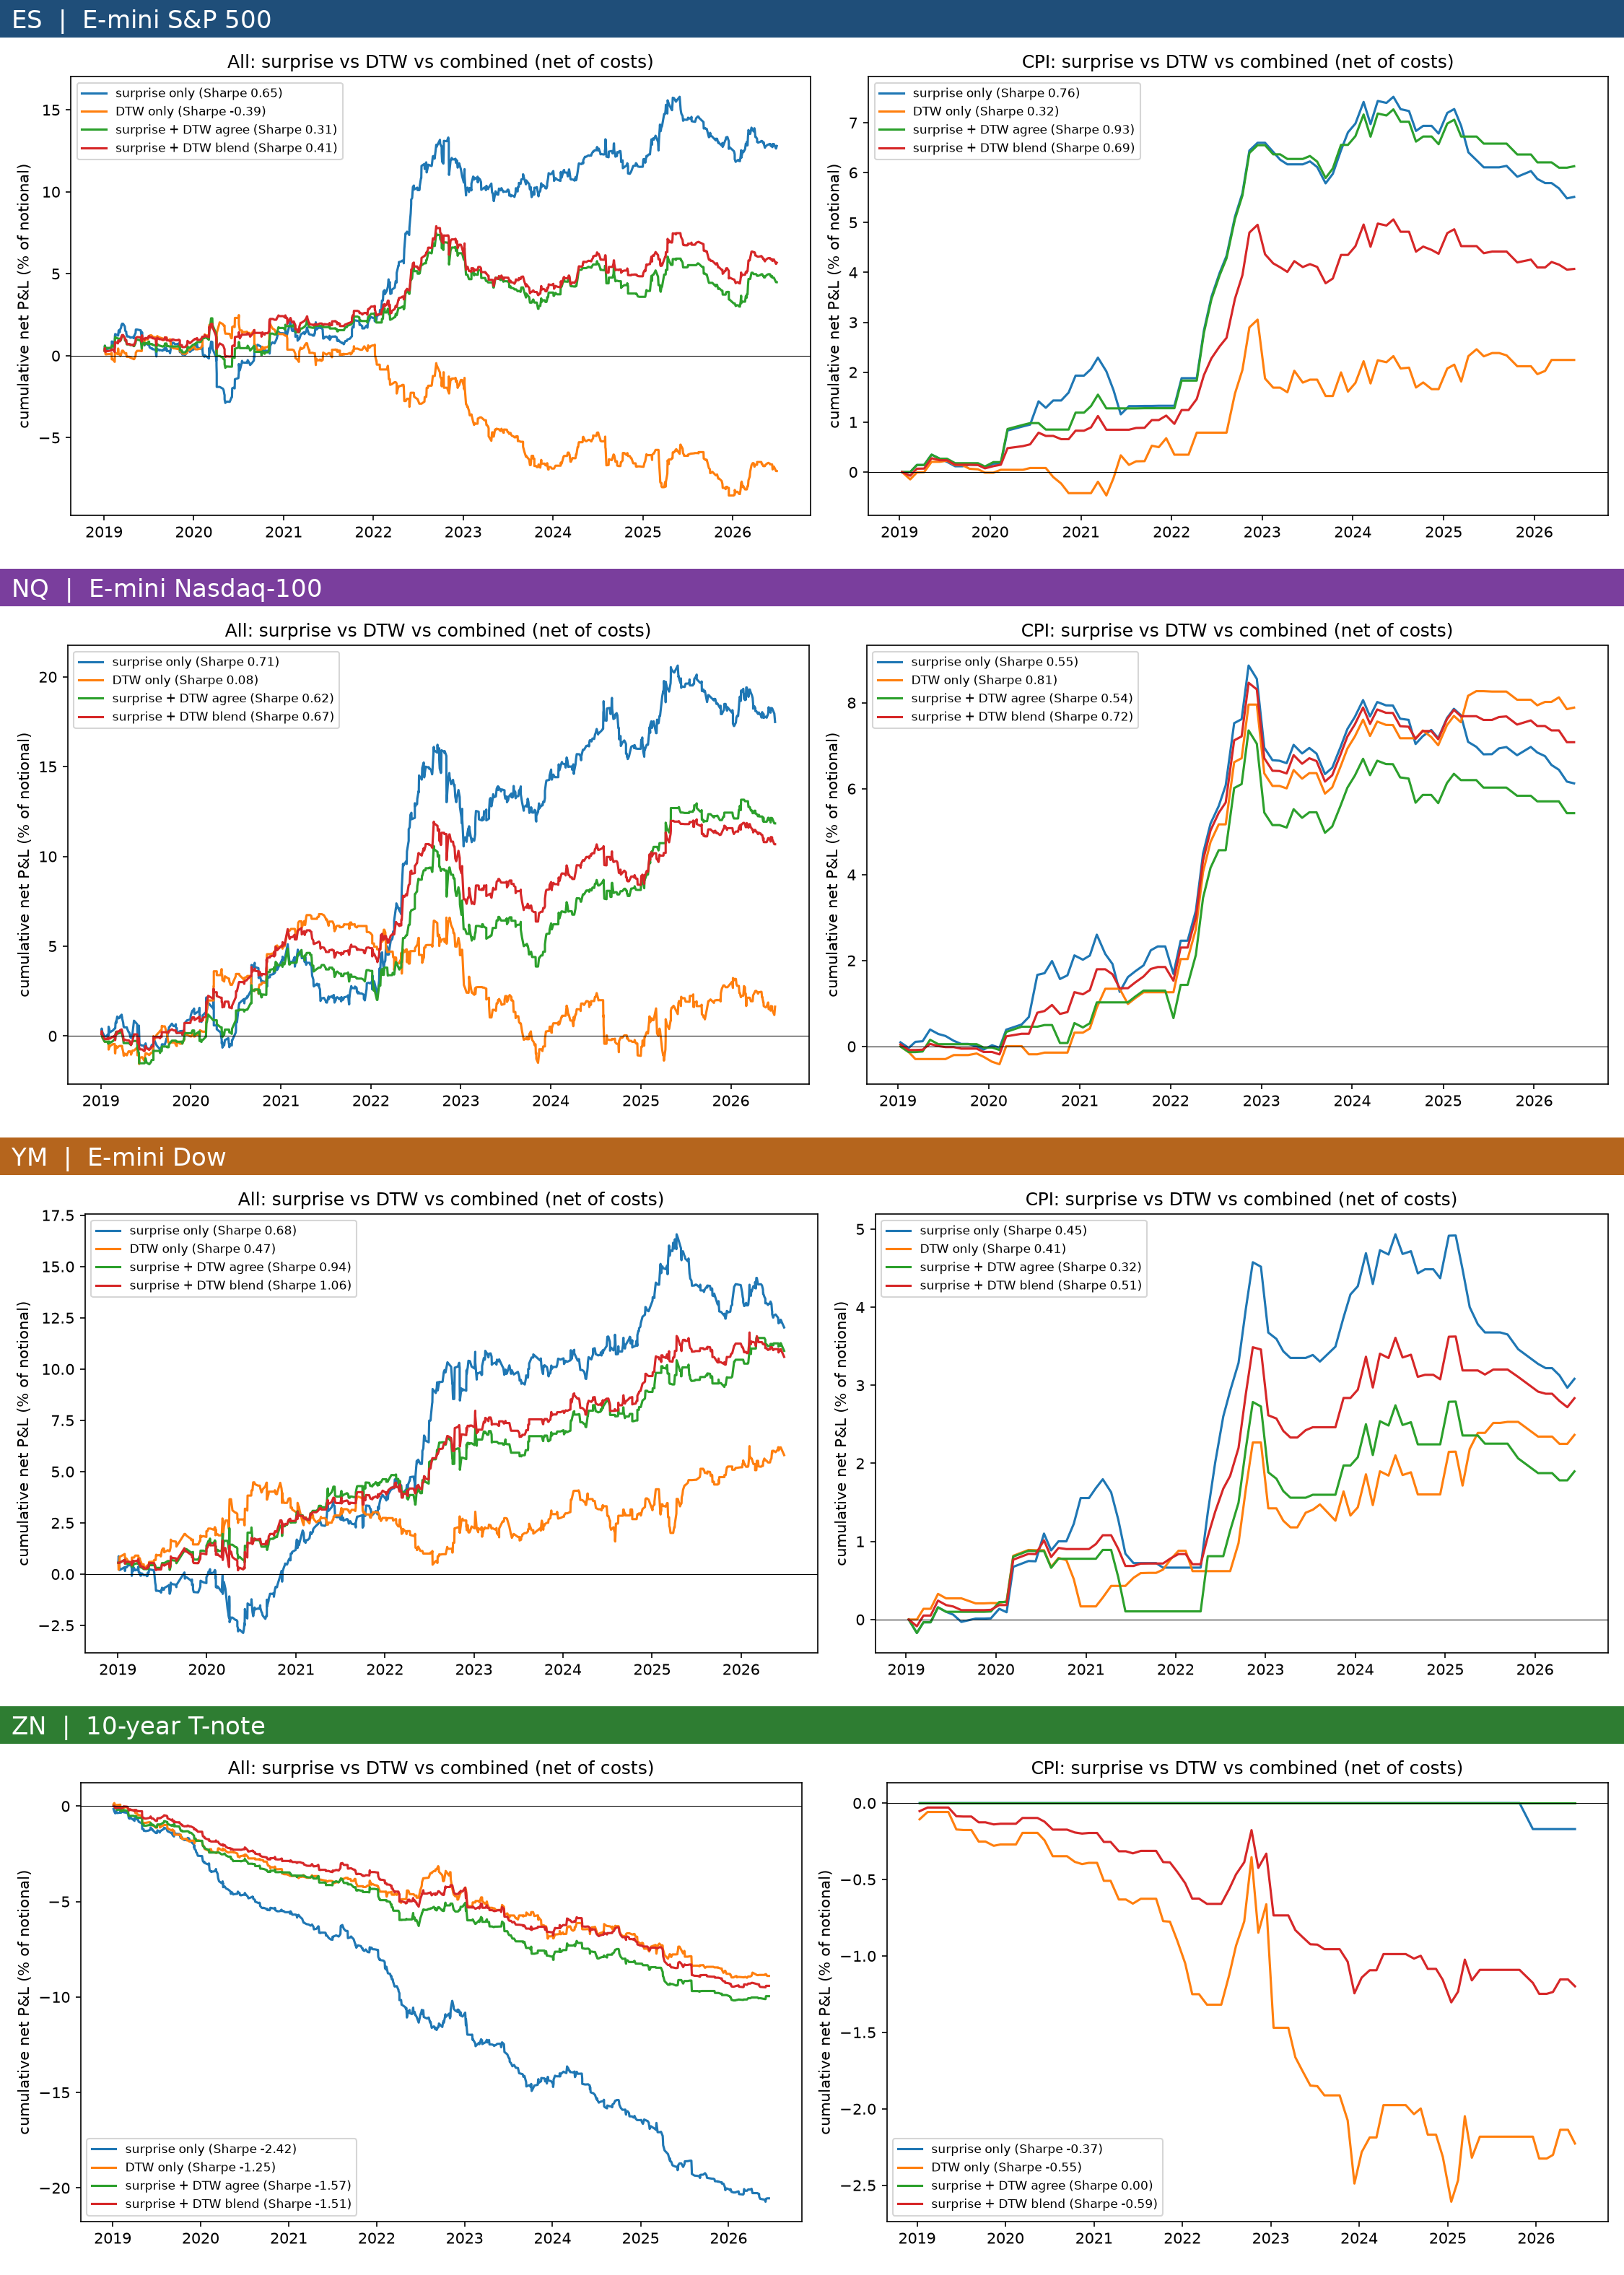
\includegraphics[width=0.82\linewidth]{app_nb06_cumulative_4markets}
  \caption{Cumulative net P\&L of the surprise-only, DTW-only, surprise + DTW agree and surprise + DTW
  blend books on all screened releases (left) and on CPI (right), 2019--2026.}
  \label{fig:app_nb06_cum}
\end{figure}

\paragraph{The ladder: can we reach about 185 trades a year? (notebook 06, section 10).} The
peer DTW strategy trades about 185 times a year on \ES\ because it takes five consecutive
30-minute trades after each release; our books take one trade per release, which caps them at about
100 trades a year. To answer the supervisor's question directly---if we trade five windows after
each release, how many trades do we get, and what happens to the Sharpe ratio?---notebook 06 copies
the ladder structure onto the same releases as the broad surprise book (Table~\ref{tab:app_ladder_design}).
The design was fixed before running. In window $k$ the DTW path is the 31 minutes ending at that
window's entry, matched against earlier releases at the same clock time, and the neighbours'
window-$k$ returns are the forecast; neighbours must have finished window $k$ before the current
release, and the gate is computed separately for each window. The surprise rule holds the sign of
the release's surprise in each window. Every window pays the same round-trip cost. Three books are
compared: a DTW ladder (DTW in all five windows, closest to the peer), a surprise ladder (the surprise
in all five), and the surprise in the first window followed by DTW in windows 2--5. Because the
surprise's effect was already gone in the second window and DTW showed no direction in the first,
we expected the trade count to reach the peer's level while the Sharpe ratio fell toward zero.

\begin{table}[!htb]
  \centering\small
  \caption{Ladder design: five back-to-back windows per release.}\label{tab:app_ladder_design}
  \begin{tabular}{ccc}
    \toprule
    Window & Entry $\to$ exit (bars after the release) & Clock time for an 08:30 release \\
    \midrule
    1 & close of bar $T$ $\to$ $T+29$ & 08:31 $\to$ 09:00 \\
    2 & $T+29 \to T+59$ & 09:00 $\to$ 09:30 \\
    3 & $T+59 \to T+89$ & 09:30 $\to$ 10:00 \\
    4 & $T+89 \to T+119$ & 10:00 $\to$ 10:30 \\
    5 & $T+119 \to T+149$ & 10:30 $\to$ 11:00 \\
    \bottomrule
  \end{tabular}
  \par\smallskip\footnotesize Later windows of an 08:30 release can overlap the first window of a
  10:00 release on the same day; each window is a separate one-contract trade, as in the peer strategy.
\end{table}

The expectation held (Table~\ref{tab:app_ladder_books}, Figure~\ref{fig:app_ladder}). The ladders
reach 300--490 trades a year, well above the peer's 185, but every one earns less than the single
first-window surprise book, and in \ES\ and \ZN\ all of them lose heavily (\ES: $-1.23$, $-1.00$ and
$-0.75$). In \NQ\ the surprise in the first window followed by DTW keeps 0.27, and in \YM\ it is flat.
The extra trades also lower the hit rate below 50\% in \ES\ and \ZN, turn the net return per
trade negative, and raise the maximum drawdown from about $-5\%$ to between $-10\%$ and $-51\%$ in the
equity indices; none of the ladder directions beats random signs at 5\%. More trades per release add
cost, not information. The peer's 185 trades a year with a Sharpe ratio of 0.61 come from its own
release set and setting; on our releases, copying its structure does not reproduce its result.

\begin{table}[!htb]
  \centering\footnotesize
  \caption{Ladder books: trade count against Sharpe ratio (notebook 06, section 10.4), 2019--2026,
  2 ticks + \$4.50.}\label{tab:app_ladder_books}
  \setlength{\tabcolsep}{3pt}
  \begin{tabular}{llcccccccc}
    \toprule
    & Book & Trades/yr & Hit & bps/trade & Total & Sharpe & Ex-2022 & Max DD & $p$ (random) \\
    \midrule
    \ES & Surprise, window 1 only & 98 & 51\% & 1.74 & 12.8\% & 0.65 & 0.28 & $-4.8$\% & 0.00 \\
     & DTW ladder & 314 & 46\% & $-2.06$ & $-48.4$\% & $-1.23$ & $-1.09$ & $-51.2$\% & 0.80 \\
     & Surprise ladder & 490 & 46\% & $-1.15$ & $-42.4$\% & $-1.00$ & $-1.08$ & $-45.6$\% & 0.34 \\
     & Surprise W1 + DTW W2--5 & 348 & 47\% & $-1.10$ & $-28.6$\% & $-0.75$ & $-0.80$ & $-30.1$\% & 0.27 \\
    \midrule
    \NQ & Surprise, window 1 only & 97 & 53\% & 2.41 & 17.5\% & 0.71 & 0.44 & $-5.7$\% & 0.00 \\
     & DTW ladder & 309 & 50\% & $-0.13$ & $-2.9$\% & $-0.07$ & $-0.17$ & $-24.2$\% & 0.28 \\
     & Surprise ladder & 484 & 50\% & $-0.39$ & $-14.3$\% & $-0.29$ & $-0.21$ & $-23.6$\% & 0.43 \\
     & Surprise W1 + DTW W2--5 & 342 & 51\% & 0.50 & 12.9\% & 0.27 & $-0.04$ & $-15.6$\% & 0.06 \\
    \midrule
    \YM & Surprise, window 1 only & 93 & 53\% & 1.73 & 12.0\% & 0.68 & 0.40 & $-4.5$\% & 0.01 \\
     & DTW ladder & 298 & 50\% & $-0.28$ & $-6.1$\% & $-0.23$ & $-0.14$ & $-12.4$\% & 0.18 \\
     & Surprise ladder & 463 & 50\% & $-0.41$ & $-14.2$\% & $-0.34$ & $-0.44$ & $-17.3$\% & 0.15 \\
     & Surprise W1 + DTW W2--5 & 329 & 50\% & 0.00 & 0.1\% & 0.00 & $-0.14$ & $-10.2$\% & 0.06 \\
    \midrule
    \ZN & Surprise, window 1 only & 82 & 36\% & $-3.35$ & $-20.5$\% & $-2.42$ & $-2.53$ & $-20.6$\% & 0.81 \\
     & DTW ladder & 267 & 32\% & $-2.70$ & $-54.1$\% & $-3.92$ & $-4.59$ & $-54.2$\% & 0.10 \\
     & Surprise ladder & 410 & 30\% & $-3.13$ & $-96.1$\% & $-7.65$ & $-8.32$ & $-96.1$\% & 1.00 \\
     & Surprise W1 + DTW W2--5 & 294 & 32\% & $-2.98$ & $-65.7$\% & $-5.35$ & $-6.27$ & $-65.6$\% & 0.89 \\
    \midrule
    & Peer: DTW ladder (slide, \ES, 2018--2026) & 185 & -- & 1.18 & 18.6\% & 0.61 & -- & $-4.9$\% & -- \\
    \bottomrule
  \end{tabular}
  \par\smallskip\footnotesize Net bps per trade; total net return in \% of notional; $p$: share of
  random-sign books with a Sharpe ratio at least as high.
\end{table}

\begin{figure}[!htb]
  \centering
  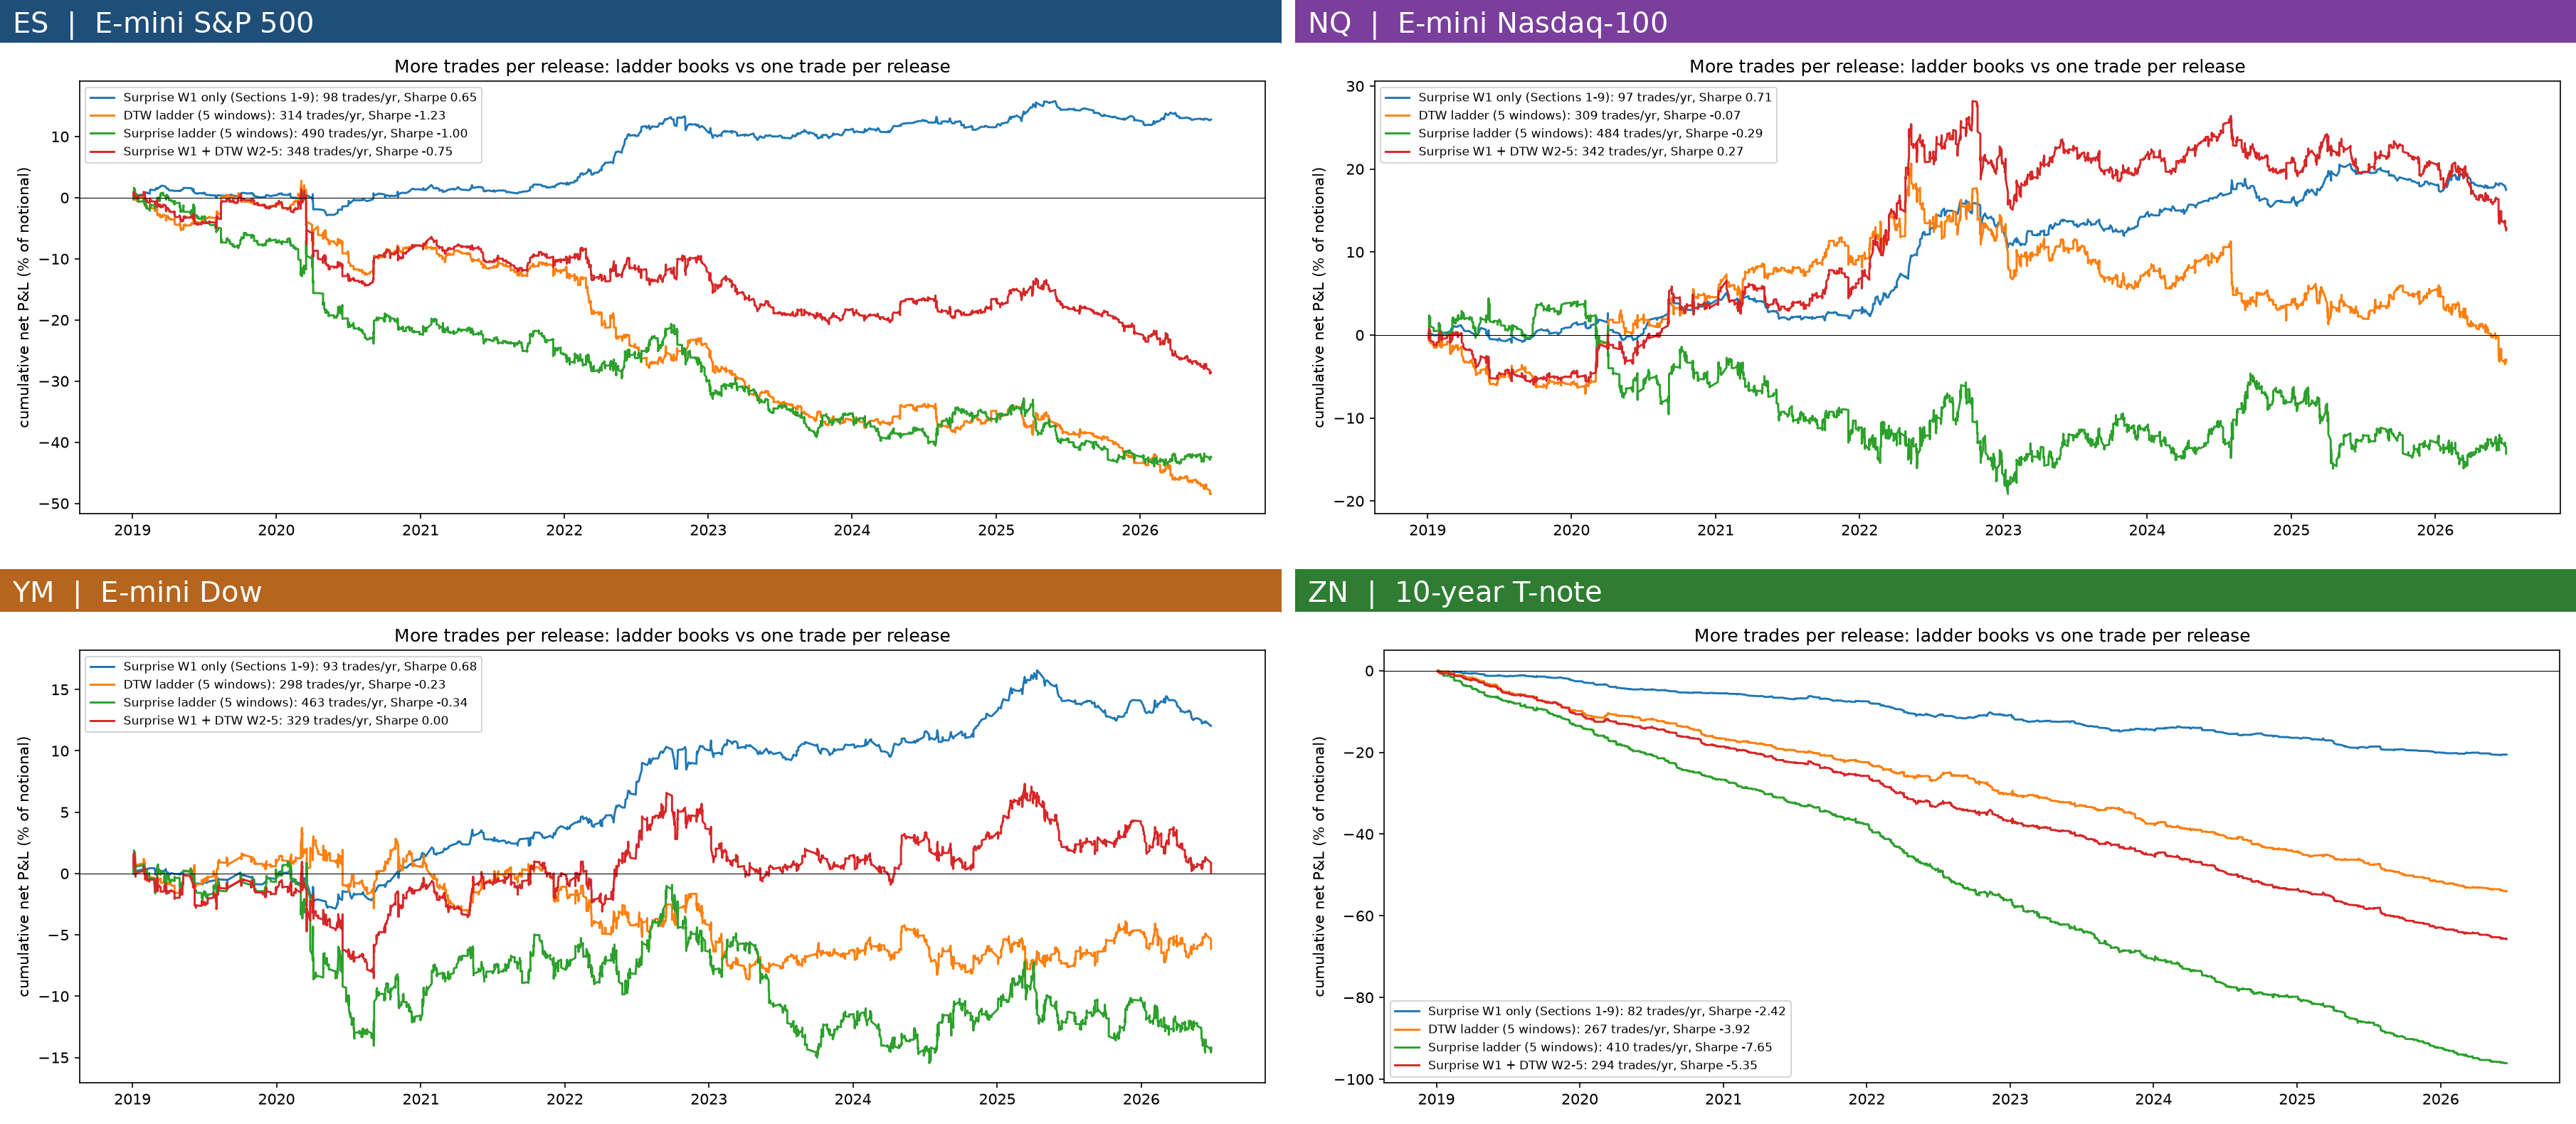
\includegraphics[width=\linewidth]{app_ladder_cumulative_4markets}
  \caption{Cumulative net P\&L of the five-window ladders (surprise, DTW, and surprise in the first
  window with DTW afterwards) against the single first-window surprise book, 2019--2026.}
  \label{fig:app_ladder}
\end{figure}

\paragraph{Results by window (notebook 06, section 10.3).} Table~\ref{tab:app_ladder_window} scores
each window on its own. The surprise has information only in the first window: its rank correlation
with the next 30-minute return is 0.14 in \ES, 0.09 in \NQ\ and \YM, and then falls to between $-0.06$
and $+0.05$ in windows 2--5, where every surprise window loses. DTW has no consistent information in
any window in \ES\ and \NQ\ (rank correlations of $-0.05$ to $+0.03$); in \YM\ its first window has a
rank correlation of 0.07 and a Sharpe ratio of 0.47, and the later windows fade. In \ZN\ every
window loses under both rules. The per-window Sharpe ratios are shown in Figure~\ref{fig:ladder} of
the main text.

\begin{table}[!htb]
  \centering\small
  \caption{Each ladder window on its own: rank correlation with the next 30-minute return and net
  Sharpe ratio, 2019--2026.}\label{tab:app_ladder_window}
  \setlength{\tabcolsep}{3pt}
  \begin{tabular}{llccccc}
    \toprule
    Market & Rule & Window 1 & Window 2 & Window 3 & Window 4 & Window 5 \\
    \midrule
    \ES & Surprise & 0.14 / 0.65 & 0.01 / $-0.79$ & $-0.06$ / $-0.57$ & 0.00 / $-0.57$ & 0.01 / $-1.16$ \\
        & DTW & 0.01 / $-0.39$ & $-0.02$ / $-0.96$ & 0.01 / $-0.38$ & 0.03 / $-0.22$ & $-0.05$ / $-1.29$ \\
    \NQ & Surprise & 0.09 / 0.71 & $-0.01$ / $-0.23$ & $-0.06$ / $-0.50$ & 0.02 / 0.23 & $-0.04$ / $-0.96$ \\
        & DTW & 0.03 / 0.08 & $-0.01$ / 0.01 & $-0.01$ / $-0.23$ & 0.02 / 0.15 & $-0.01$ / $-0.18$ \\
    \YM & Surprise & 0.09 / 0.68 & 0.05 / $-0.15$ & 0.02 / $-0.18$ & $-0.06$ / $-0.80$ & 0.04 / $-0.30$ \\
        & DTW & 0.07 / 0.47 & 0.03 / $-0.19$ & 0.05 / 0.15 & 0.01 / 0.03 & $-0.06$ / $-1.03$ \\
    \ZN & Surprise & $-0.03$ / $-2.42$ & $-0.01$ / $-3.08$ & 0.01 / $-3.15$ & $-0.04$ / $-3.90$ & 0.04 / $-3.56$ \\
        & DTW & 0.04 / $-1.25$ & $-0.02$ / $-1.94$ & $-0.02$ / $-2.34$ & 0.01 / $-1.62$ & $-0.01$ / $-2.92$ \\
    \bottomrule
  \end{tabular}
  \par\smallskip\footnotesize Each cell: rank correlation / net Sharpe ratio.
\end{table}

\FloatBarrier
\subsection{Multi-market surprise book (notebook 07)}

\paragraph{Performance by market (notebook 07, section 5).} Figure~\ref{fig:app_perf_market} and
Table~\ref{tab:app_perf_market} run the same five books, with the same code and constants, on each
market. The pattern is the same in the three equity indices and opposite in \ZN. The broad naive
surprise book earns 0.65 in \ES, 0.71 in \NQ\ and 0.68 in \YM, with random-sign $p$-values of 0.006 or
below; the CPI model 0.45--0.76; and keeping CPI trades only when DTW agrees 0.32--0.93, on six or
seven trades a year. The DTW-only book loses in \ES, is flat in \NQ\ and earns 0.47 in \YM. Gross
against net Sharpe ratios show what costs take: about 0.5 in \ES, 0.2 in \NQ\ and 0.3 in \YM\ for the
broad book, but 2.1 in \ZN, where the naive book goes from $-0.30$ before costs to $-2.42$ after them. Over the
cost grid the broad book's Sharpe ratio falls from 1.09 to 0.20 in \ES\ as slippage rises from zero
to four ticks, but only from 0.82 to 0.60 in \NQ\ and from 0.91 to 0.45 in \YM, because the \NQ\ and
\YM\ ticks are smaller relative to their moves.

\begin{table}[!htb]
  \centering\small
  \caption{Performance by market, 2019--2026, 2 ticks + \$4.50: net Sharpe ratio (gross in
  parentheses) and trades per year.}\label{tab:app_perf_market}
  \begin{threeparttable}
  \setlength{\tabcolsep}{4pt}
  \begin{tabular}{lcccc}
    \toprule
    Book & \ES & \NQ & \YM & \ZN \\
    \midrule
    All $\cdot$ naive & 0.65 (1.17) & 0.71 (0.87) & 0.68 (1.01) & $-2.42$ ($-0.30$) \\
    \quad trades / yr; $p$ (random sign) & 98; 0.000 & 97; 0.005 & 93; 0.006 & 82; 0.81 \\
    All $\cdot$ DTW only & $-0.39$ ($-0.01$) & 0.08 (0.21) & 0.47 (0.79) & $-1.25$ (0.47) \\
    All $\cdot$ surprise + DTW agree & 0.31 (0.70) & 0.62 (0.73) & 0.94 (1.21) & $-1.57$ ($-0.12$) \\
    CPI $\cdot$ surprise model & 0.76 (0.88) & 0.55 (0.60) & 0.45 (0.53) & $-0.37$ (1 trade) \\
    CPI $\cdot$ surprise + DTW agree & 0.93 (1.02) & 0.54 (0.57) & 0.32 (0.38) & -- \\
    \midrule
    All $\cdot$ naive, Sharpe without 2022 & 0.28 & 0.44 & 0.40 & $-2.53$ \\
    \midrule
    \multicolumn{5}{l}{\emph{All $\cdot$ naive, net Sharpe by round-trip slippage (plus \$4.50)}} \\
    0 ticks & 1.09 & 0.82 & 0.91 & $-0.56$ \\
    1 tick  & 0.87 & 0.77 & 0.80 & $-1.49$ \\
    2 ticks & 0.65 & 0.71 & 0.68 & $-2.42$ \\
    4 ticks & 0.20 & 0.60 & 0.45 & $-4.24$ \\
    \bottomrule
  \end{tabular}
  \begin{tablenotes}\footnotesize
    \item Notes: Monthly Sharpe ratios; ``--'': no trades. The \ZN\ CPI model trades about once over
    the sample, because its predicted drift rarely exceeds the cost.
  \end{tablenotes}
  \end{threeparttable}
\end{table}

\begin{figure}[!htb]
  \centering
  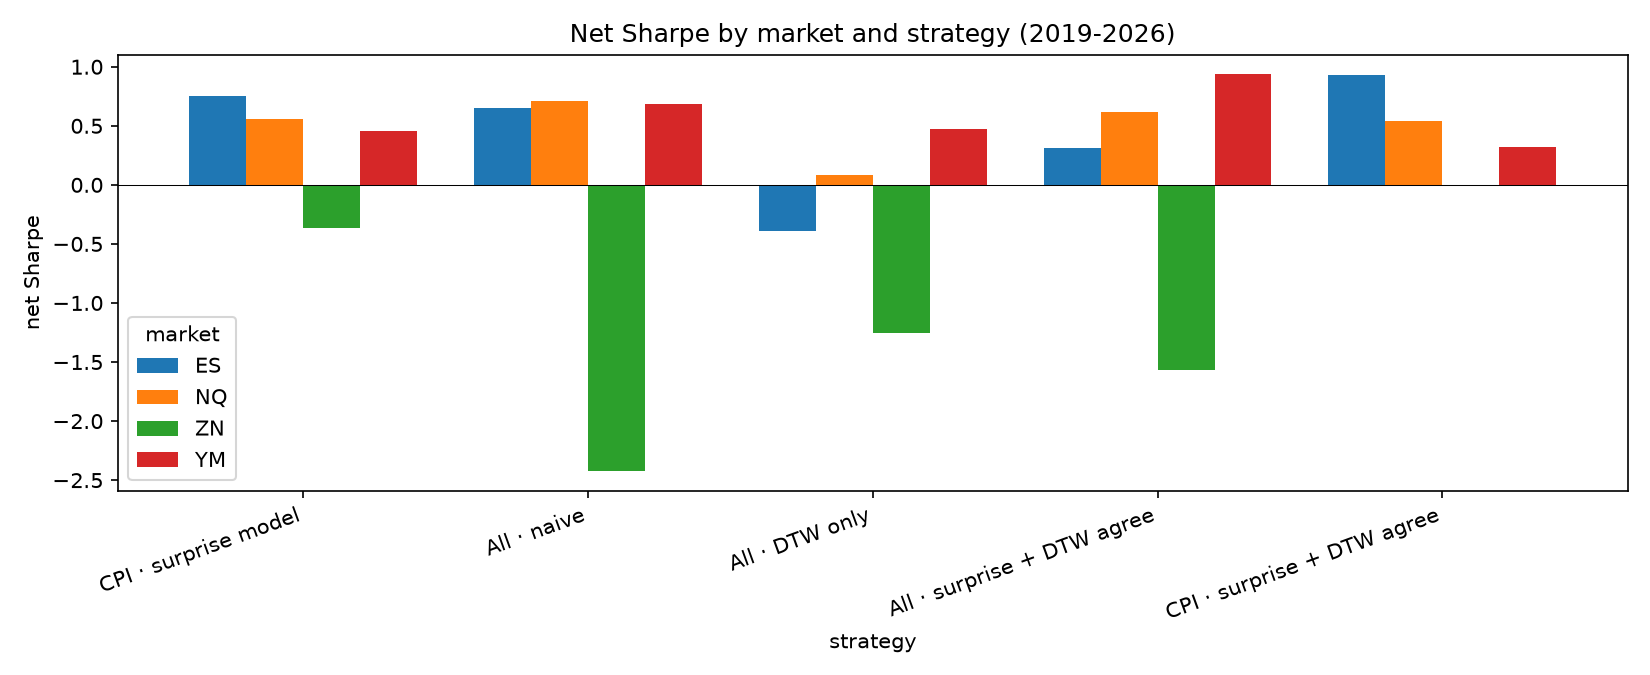
\includegraphics[width=0.85\linewidth]{app_nb07b_sharpe_by_market}
  \caption{Net Sharpe ratio by market and strategy, 2019--2026, 2 ticks + \$4.50 (notebook 07,
  section 5).}
  \label{fig:app_perf_market}
\end{figure}

\paragraph{Portfolios: all markets, equities and \ES\ + \NQ\ (notebook 07, sections 5--6).}
Table~\ref{tab:app_portfolios07} and Figure~\ref{fig:app_multi} combine the per-market books with
equal-risk weights fixed on 2016--2018 (\ES\ 1.00, \NQ\ 0.71, \YM\ 1.02, \ZN\ 2.67). Adding \YM\ to \ES\ and
\NQ\ improves the multi-release equity book: the Sharpe ratio rises from 0.72 to 0.78, total net P\&L
from 25\% to 38\%, trades from 195 to 288 a year, and the 90\% confidence interval moves fully above
zero (0.10 to 1.50). The Sharpe ratio without 2022 also rises (0.38 to 0.43). The cost is a larger
drawdown ($-9.2\%$ against $-7.4\%$), because the book is bigger. \YM\ helps because its monthly
returns correlate only 0.66 with \ES's and 0.43 with \NQ's. For the CPI-only model \YM\ adds little
(0.69 to 0.63), because the CPI books of the three indices are highly correlated. \ZN\ breaks every
portfolio it enters: equal-risk weighting gives it the largest weight (2.67, because its moves are
small), its multi-release book loses ($-2.42$), and the four-market naive book is negative ($-0.34$,
drawdown $-23\%$). \ZN\ should therefore be excluded from the traded book. The four-market CPI
portfolio still earns 0.61 because the CPI model almost never trades \ZN.

\begin{table}[!htb]
  \centering\small
  \caption{Equal-risk surprise portfolios across markets, 2019--2026, 2 ticks + \$4.50 (weights fixed
  on 2016--2018: \ES\ 1.00, \NQ\ 0.71, \YM\ 1.02, \ZN\ 2.67).}\label{tab:app_portfolios07}
  \setlength{\tabcolsep}{3pt}
  \begin{tabular}{lccccccc}
    \toprule
    Portfolio & Trades/yr & Sharpe & 90\% CI & Ex-2022 & Total & Max DD & $p$ (random) \\
    \midrule
    \ES+\NQ, all $\cdot$ naive & 195 & 0.72 & [$-0.01$, 1.43] & 0.38 & 25.2\% & $-7.4\%$ & 0.000 \\
    \textbf{Equities (\ES+\NQ+\YM), all $\cdot$ naive} & \textbf{288} & \textbf{0.78} & \textbf{[0.10, 1.50]} & \textbf{0.43} & \textbf{37.5\%} & $-9.2\%$ & \textbf{0.000} \\
    \ES+\NQ, CPI model & 20 & 0.69 & [$-0.01$, 1.39] & 0.02 & 9.9\% & $-3.3\%$ & 0.023 \\
    Equities (\ES+\NQ+\YM), CPI model & 29 & 0.63 & [$-0.10$, 1.37] & $-0.04$ & 13.0\% & $-5.3\%$ & 0.020 \\
    All four markets, all $\cdot$ naive & 370 & $-0.34$ & [$-1.08$, 0.40] & $-0.74$ & $-17.4\%$ & $-23.4\%$ & 0.000 \\
    All four markets, CPI model & 29 & 0.61 & [$-0.13$, 1.35] & $-0.07$ & 12.6\% & $-5.8\%$ & 0.018 \\
    \midrule
    All four markets, DTW only & 244 & $-0.64$ & [$-1.28$, $-0.01$] & $-0.62$ & $-23.7\%$ & $-29.1\%$ & 0.028 \\
    All four markets, surprise + DTW agree & 195 & $-0.07$ & [$-0.74$, 0.61] & $-0.29$ & $-2.6\%$ & $-15.6\%$ & 0.001 \\
    All four markets, CPI + DTW agree & 19 & 0.67 & [$-0.01$, 1.31] & $-0.01$ & 11.9\% & $-3.4\%$ & 0.010 \\
    \bottomrule
  \end{tabular}
  \par\smallskip\footnotesize Total net return in \% of \ES-equivalent notional. For the four-market
  naive book, the random-sign $p$ of 0.000 says its direction is better than random; the loss comes
  from \ZN's costs, which random-sign books pay too.
\end{table}

\begin{figure}[!htb]
  \centering
  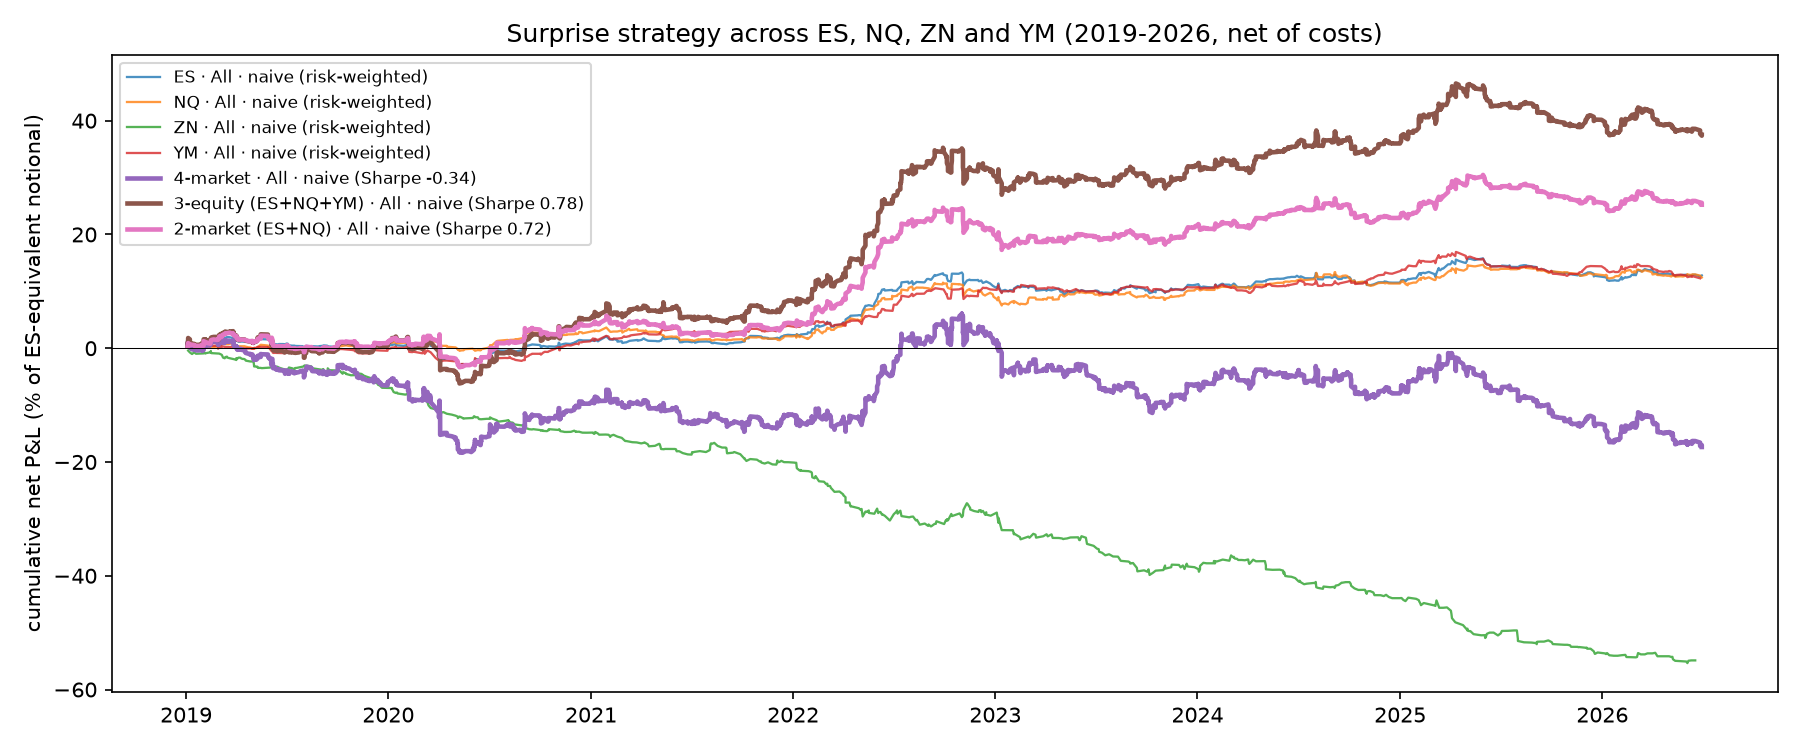
\includegraphics[width=0.8\linewidth]{app_nb07b_portfolio_cumulative}
  \caption{Cumulative net P\&L of the risk-weighted surprise books (broad naive book) by market and
  of the two-, three- and four-market portfolios, 2019--2026.}
  \label{fig:app_multi}
\end{figure}

\paragraph{Final comparison (notebook 07, section 7).} Table~\ref{tab:app_final07} brings every
market and portfolio book of notebook 07 together. It summarizes the notebook's conclusion: the
consensus surprise is the source of direction in all three equity indices, the broad naive book is
the most robust single book (positive without 2022 and significant against random signs in each
index), the three-index portfolio is the best overall, and \ZN\ should not be traded at these costs.

\begin{table}[!htb]
  \centering\footnotesize
  \caption{Final comparison of the multi-market surprise books, 2019--2026, 2 ticks + \$4.50
  (notebook 07, section 7).}\label{tab:app_final07}
  \setlength{\tabcolsep}{4pt}
  \begin{tabular}{lcccccc}
    \toprule
    Book & Trades/yr & bps/trade & Sharpe & Ex-2022 & Max DD & $p$ (random) \\
    \midrule
    \ES\ $\cdot$ CPI $\cdot$ surprise model & 9 & 8.23 & 0.76 & 0.05 & $-2.0\%$ & 0.006 \\
    \ES\ $\cdot$ All $\cdot$ naive & 98 & 1.74 & 0.65 & 0.28 & $-4.8\%$ & 0.000 \\
    \ES\ $\cdot$ All $\cdot$ surprise + DTW agree & 53 & 1.14 & 0.31 & 0.07 & $-4.6\%$ & 0.030 \\
    \ES\ $\cdot$ All $\cdot$ DTW only & 65 & $-1.45$ & $-0.39$ & $-0.32$ & $-11.0\%$ & 0.479 \\
    \midrule
    \NQ\ $\cdot$ CPI $\cdot$ surprise model & 11 & 7.12 & 0.55 & $-0.01$ & $-2.7\%$ & 0.047 \\
    \NQ\ $\cdot$ All $\cdot$ naive & 97 & 2.41 & 0.71 & 0.44 & $-5.7\%$ & 0.005 \\
    \NQ\ $\cdot$ All $\cdot$ surprise + DTW agree & 51 & 3.11 & 0.62 & 0.59 & $-6.7\%$ & 0.021 \\
    \NQ\ $\cdot$ All $\cdot$ DTW only & 63 & 0.34 & 0.08 & 0.17 & $-8.3\%$ & 0.271 \\
    \midrule
    \YM\ $\cdot$ CPI $\cdot$ surprise model & 9 & 4.67 & 0.45 & $-0.15$ & $-2.0\%$ & 0.060 \\
    \YM\ $\cdot$ All $\cdot$ naive & 93 & 1.73 & 0.68 & 0.40 & $-4.5\%$ & 0.006 \\
    \YM\ $\cdot$ All $\cdot$ surprise + DTW agree & 49 & 2.94 & 0.94 & 0.94 & $-1.7\%$ & 0.002 \\
    \YM\ $\cdot$ All $\cdot$ DTW only & 61 & 1.27 & 0.47 & 0.58 & $-4.0\%$ & 0.024 \\
    \midrule
    \ZN\ $\cdot$ CPI $\cdot$ surprise model & 0 & $-17.03$ & $-0.37$ & $-0.39$ & $-0.2\%$ & 1.000 \\
    \ZN\ $\cdot$ All $\cdot$ naive & 82 & $-3.35$ & $-2.42$ & $-2.53$ & $-20.6\%$ & 0.812 \\
    \ZN\ $\cdot$ All $\cdot$ surprise + DTW agree & 42 & $-3.18$ & $-1.57$ & $-1.89$ & $-10.2\%$ & 0.645 \\
    \ZN\ $\cdot$ All $\cdot$ DTW only & 55 & $-2.15$ & $-1.25$ & $-1.71$ & $-9.1\%$ & 0.164 \\
    \midrule
    2-market (\ES+\NQ) $\cdot$ All $\cdot$ naive & 195 & 1.73 & 0.72 & 0.38 & $-7.4\%$ & 0.000 \\
    2-market (\ES+\NQ) $\cdot$ CPI $\cdot$ surprise model & 20 & 6.45 & 0.69 & 0.02 & $-3.3\%$ & 0.023 \\
    \midrule
    3-equity (\ES+\NQ+\YM) $\cdot$ All $\cdot$ naive & 288 & 1.74 & 0.78 & 0.43 & $-9.2\%$ & 0.000 \\
    3-equity (\ES+\NQ+\YM) $\cdot$ CPI $\cdot$ surprise model & 29 & 5.94 & 0.63 & $-0.04$ & $-5.3\%$ & 0.020 \\
    \midrule
    4-market $\cdot$ CPI $\cdot$ surprise model & 29 & 5.71 & 0.61 & $-0.07$ & $-5.8\%$ & 0.018 \\
    4-market $\cdot$ All $\cdot$ naive & 370 & $-0.63$ & $-0.34$ & $-0.74$ & $-23.4\%$ & 0.000 \\
    4-market $\cdot$ All $\cdot$ DTW only & 244 & $-1.30$ & $-0.64$ & $-0.62$ & $-29.1\%$ & 0.028 \\
    4-market $\cdot$ All $\cdot$ surprise + DTW agree & 195 & $-0.18$ & $-0.07$ & $-0.29$ & $-15.6\%$ & 0.001 \\
    4-market $\cdot$ CPI $\cdot$ surprise + DTW agree & 19 & 8.17 & 0.67 & $-0.01$ & $-3.4\%$ & 0.010 \\
    \bottomrule
  \end{tabular}
  \par\smallskip\footnotesize Net bps per trade; monthly Sharpe ratios; $p$: share of random-sign
  books with a Sharpe ratio at least as high.
\end{table}





\end{document}
